%%%%%%%%%%%%%%%%%%%%%%%%%%%%%%%%%%%%%%%%%%%%%%%%%%%%%%%%%%%%%%%%%%%%%%%%%%
%
% STAR Class Library - User Guide and Reference Manual -- LaTeX Source 
%
% $Id: StarClassLibrary.tex,v 1.11 1999/10/06 13:40:30 ullrich Exp $
%
% Author: LaTeX template by Thomas Ullrich, March 19 1998
%
%%%%%%%%%%%%%%%%%%%%%%%%%%%%%%%%%%%%%%%%%%%%%%%%%%%%%%%%%%%%%%%%%%%%%%%%%%
%
% $Log: StarClassLibrary.tex,v $
% Revision 1.11  1999/10/06 13:40:30  ullrich
% Corrected explanation of MACROs.
%
% Revision 1.19  2000/04/06 23:01:45  ullrich
% Added reference section for StMath. Particle section updated.
%
% Revision 1.18  2000/03/16 16:31:48  ullrich
% Added description of StRandom.
%
% Revision 1.17  2000/03/06 20:25:49  ullrich
% Added text to StHelix reference. More details on the
% case B=0 (concerning parameter h and the phase).
%
% Revision 1.16  2000/03/06 19:23:40  ullrich
% Added description of convention h=+1 for case B=0.
%
% Revision 1.15  2000/02/28 19:38:43  ullrich
% Added the hyperref package to add bookmarks and hyperlinks
% to pdf output files.
%
% Revision 1.14  1999/12/21 16:41:13  ullrich
% Added StFastCircleFitter docu.
%
% Revision 1.13  1999/11/18 17:57:24  ullrich
% Fixed some typos
%
% Revision 1.12  1999/11/10 12:37:11  ullrich
% Added description of StMemoryPool.
%
% Revision 1.11  1999/10/06 13:40:30  ullrich
% Corrected explanation of MACROs.
%
% Revision 1.10  1999/09/29 16:54:46  ullrich
% Added graphics to explain StThreeVector.
%
% Revision 1.9  1999/09/23 12:09:44  ullrich
% New section on the question of helix parameters
%
% Revision 1.8  1999/06/04 18:07:09  ullrich
% Added description of new class StMemoryInfo.
% Update of StThreeVector and StLorentzVector.
%
% Revision 1.7  1999/05/17 11:10:00  ullrich
% Added documentation on particle definitions
%
% Revision 1.6  1999/04/28 16:14:13  ullrich
% Added more examples
%
% Revision 1.5  1999/04/27 19:58:08  ullrich
% Added description of StTimer
%
% Revision 1.4  1999/03/30 19:06:25  ullrich
% Added description of dca between two helices to
% appendix. Corrected some typos.
%
% Revision 1.3  1999/03/11 13:07:13  ullrich
% Change of package names to cope with newer versions of LaTeX.
%
% Revision 1.2  1999/03/02 23:18:08  ullrich
% Modified 'User Guide' for new SCL organization scheme.
% Updated StHelix reference page.
%
% Revision 1.1  1999/02/17 12:37:56  ullrich
% New Revision
%
%%%%%%%%%%%%%%%%%%%%%%%%%%%%%%%%%%%%%%%%%%%%%%%%%%%%%%%%%%%%%%%%%%%%%%%%%%
\documentclass[twoside]{article}

\parskip 6pt
\advance\textwidth by 80pt%
\advance\evensidemargin by -80pt%

%\renewcommand{\familydefault}{cmss}

\usepackage{graphicx}
\usepackage{psboxit}
\usepackage{color}
\usepackage{amsmath}
\usepackage{amssymb}
\usepackage{fancyhdr}
\usepackage{times}
\usepackage{verbatim}
\usepackage{makeidx}
\usepackage{subfigure}
\usepackage[dvips=true,hyperindex=true,colorlinks=true,linkcolor=blue,bookmarks=true]{hyperref}

\PScommands      % init boxit
\makeindex

%%%%%%%%%%%%%%%%%%%%%%%%%%%%%%%%%%%%%%%%%%%%%%%%%%%%%%%%%%%%%%%%%%%%
%
% Define header and footer style
%
%%%%%%%%%%%%%%%%%%%%%%%%%%%%%%%%%%%%%%%%%%%%%%%%%%%%%%%%%%%%%%%%%%%%
\pagestyle{fancyplain}
\rhead[\fancyplain{}{\bfseries\leftmark}]
      {\fancyplain{}{\bfseries\rightmark}}
\lhead[\fancyplain{}{\bfseries\rightmark}]
      {\fancyplain{}{\bfseries\leftmark}}
\rfoot[{}]{\fancyplain{}{\bfseries\thepage}}
\lfoot[\fancyplain{}{\bfseries\thepage}]{}
\cfoot{}

%%%%%%%%%%%%%%%%%%%%%%%%%%%%%%%%%%%%%%%%%%%%%%%%%%%%%%%%%%%%%%%%%%%%
%
% Typographic Conventions
%
%%%%%%%%%%%%%%%%%%%%%%%%%%%%%%%%%%%%%%%%%%%%%%%%%%%%%%%%%%%%%%%%%%%%
\newcommand{\name}[1]{\textsf{#1}}%  or class-, function-, package names
\newcommand{\comp}[1]{\texttt{#1}}%  computer font
\newcommand{\args}[1]{\textit{#1}}%   command arguments

%%%%%%%%%%%%%%%%%%%%%%%%%%%%%%%%%%%%%%%%%%%%%%%%%%%%%%%%%%%%%%%%%%%%
%
% Define multiline labels for class reference
%
%%%%%%%%%%%%%%%%%%%%%%%%%%%%%%%%%%%%%%%%%%%%%%%%%%%%%%%%%%%%%%%%%%%%
\newcommand{\entrylabel}[1]{\mbox{\textbf{{#1}}}\hfil}%
\newenvironment{entry}
{\begin{list}{}%
    {\renewcommand{\makelabel}{\entrylabel}%
     \setlength{\labelwidth}{90pt}%
     \setlength{\leftmargin}{\labelwidth}
     \advance\leftmargin by \labelsep%
      }%
    }%
  {\end{list}}

\newcommand{\Entrylabel}[1]%
{\raisebox{0pt}[1ex][0pt]{\makebox[\labelwidth][l]%
    {\parbox[t]{\labelwidth}{\hspace{0pt}\textbf{{#1}}}}}}
\newenvironment{Entry}%
{\renewcommand{\entrylabel}{\Entrylabel}\begin{entry}}%
  {\end{entry}}

\begin{document}

%%%%%%%%%%%%%%%%%%%%%%%%%%%%%%%%%%%%%%%%%%%%%%%%%%%%%%%%%%%%%%%%%%%%
%
%    Title page
%
%%%%%%%%%%%%%%%%%%%%%%%%%%%%%%%%%%%%%%%%%%%%%%%%%%%%%%%%%%%%%%%%%%%%
\begin{titlepage}
\pagestyle{empty}
\vspace*{-35mm}
\begin{center}
  \mbox{
\includegraphics[width=2cm]{StarIcon.eps}}
  {\Large\bf STAR Offline Library Long Writeup}
  \hfill\mbox{}\\[3cm]
  \mbox{
\includegraphics[width=\textwidth]{StarClassLibraryTitle.eps}}
  \hfill\mbox{}\\[3cm]
  {\LARGE User Guide and Reference Manual}\\[2cm]
  {\LARGE $ $Revision: 1.11 $ $}  \\[5mm] % replaced by cvs with current revision  
  {\LARGE $ $Date: 1999/10/06 13:40:30 $ $}  % replaced by cvs with current revision  
  \vfill
\end{center}
\cleardoublepage
\end{titlepage}
\pagenumbering{roman}

%%%%%%%%%%%%%%%%%%%%%%%%%%%%%%%%%%%%%%%%%%%%%%%%%%%%%%%%%%%%%%%%%%%%
%
%    Table of content
%
%%%%%%%%%%%%%%%%%%%%%%%%%%%%%%%%%%%%%%%%%%%%%%%%%%%%%%%%%%%%%%%%%%%%
\tableofcontents
\cleardoublepage

%%%%%%%%%%%%%%%%%%%%%%%%%%%%%%%%%%%%%%%%%%%%%%%%%%%%%%%%%%%%%%%%%%%%
%
%    User Guide
%
%%%%%%%%%%%%%%%%%%%%%%%%%%%%%%%%%%%%%%%%%%%%%%%%%%%%%%%%%%%%%%%%%%%%
\pagenumbering{arabic}
\part{User Guide}
\clearpage

\section{Philosophy and Motivation} \index{philosophy}
\label{Philosophy}

Code-reusability is often claimed to be one of the most important
benefits to be realized from Object-Oriented programming.  This 
is not really a new concept, especially in High Energy
Physics (HEP) where many Fortran subroutine libraries, most notably
CERNLIB\footnote{http://wwwcn1.cern.ch/asd/index.html}
have been used for many years.  There are however, several distinct
differences between such subroutine libraries and class libraries
which Object-Oriented languages allow.  First standardized data
structures, or containers, along with operations associated with such
objects are combined in classes.  Second, with subroutine libraries
one does not have the opportunity to extend or alter the functionality
of a routine unless the source code is available and recompilation
is possible.  On the other hand, Object-Oriented languages like C++ allows
the user to produce a derived class via inheritance which one can add
functionality through the addition of member
functions \index{member functions}
or data storage through the addition of data members.

Most C++ compilers come with what is called the ``Standard C++
Library''\index{Standard C++ Library} which defines generic container
classes (i.e.~linked lists, sorted lists, etc.) and simple algorithms
associated with these containers.  However the needs of the HEP community
are much more specialized in terms of the containers we use---things
like three- and four-vectors, random number generators, matrices, etc.,
and such objects are poorly dealt with in expensive commercial class
libraries.  It was with this motivation that  Leif L\"{o}nnblad proposed
{\em A Class Library for High Energy Physics} (CLHEP) \index{CLHEP} in C++ at the
{\em Computing in High Energy Physics} (CHEP) conference in 1992.  This library provided
basic HEP specific classes and although it went a long way in providing a
standard for C++ in HEP, C++ was not a mature nor standardized language
at the time.  Recently (December 1997) an ANSI committee has proposed
an international standardization of the C++
language\footnote{http://www.cygnus.com/misc/wp/nov97/}
which makes some components of CLHEP redundant and some other parts
unnecessarily inflexible (i.e.~adding three-vectors with elements of
different types).

For these reasons it was felt that the basic component classes of CLHEP
(like vectors and matrices) could be rewritten incorporating contemporary
new standardized features of the C++
language.  These include the use of templates, exception handling, 
namespaces, use of the Standard Template Library (STL)
\index{Standard Template Library}
\index {STL} etc.  It was also felt that additional functionality specific
to the STAR experiment could be incorporated to make this a real
STAR Class Library (SCL); things like implementing the STAR track model,
data base interfaces etc.  Even a simple interface to HBOOK is included.
The code in the SCL is written to conform to the ANSI standard
and conventions of the Standard C++ Library.  The directory 
and \texttt{Makefile} structure is modelled very closely after the
pioneering work of the GEANT4 collaboration.  Documentation is also seen as
an important component of this development.  This manual provides a detailed
description of each class, its functionality, its dependencies, as well as
a description of all user accessible member functions.  Example programs
and there expected output are also included.  More detailed examples
testing the functionality of each and every member function are provided in
the \comp{examples} directory in the library itself.  Web based documentation,
giving the user access to the header files and source code is foreseen
in the near future.

These developments have been made in consultation with the CERN LHC++
\item Red Hat Linux 5.1, Red Hat Linux 5.2: \index{Linux}
expressed interest in perhaps incorporating some of this library
in a future release.  This is also by no means a complete library and as
more and more people get involved with development, it is expected to
expand.  So look through the manual and feel free to
make any comments, good or bad to the collaboration and developers.

  \end{itemize}
\item IRIX 6.4: \index{IRIX}
  \begin{itemize}
    \item CC 7.1 and Object Space 2.0.2 for IRIX 6.3 modified.
and compiled with -n32 flag. \index{Object Space}

\section{Platforms and Compilers} \index{compiler} \index{platform}
\label{platformsAndCompilers}

Further tests on AIX are not foreseen unless there is sufficient user demand. \index{Irix} \index{AIX}
\item Red Hat Linux 5.1 to Red Hat Linux 6.0: \index{Linux}
\item HP-UX 10.20: \index{HP-UX}
    \item egcs 1.0.2 (g++) or higher. 
    \item aCC A.01.06 or higher versions. \index{aCC (HP compiler)}
    \item gcc/g++ 2.9.5.
  \end{itemize}
\item Red Hat Linux 5.1 to Red Hat Linux 6.1: \index{Linux}
  \begin{itemize}
    \item gcc/g++ 2.91.66 or higher. 
  \end{itemize}
\item Solaris 2.4--2.6: \index{Solaris}
templated member functions and a broken overloading mechanism.
    \item CC 5.0 or higher
  \end{itemize}
\end{enumerate}
Tests with Visual C++ 5.0 fail because of the lack of support of \index{Visual C++}
templated member functions and a broken overloading mechanism. Visual C++ 6.0 is not
tested yet.
Further tests on AIX and IRIX are not foreseen unless there is sufficient user demand.
\index{Irix} \index{AIX}

\section{Organization of the SCL}

All documentation, code, and header files of the SCL is contained in a
directory named \name{StarClassLibrary}.
It contains 2 further sub-directories:
\name{./examples} and \name{./doc}.

To summarize:
\vspace{-11pt}
\begin{description}
\item[\name{StarClassLibrary}] is the top directory,
\begin{description}
\item[\name{./}] contains the different header files
    (extension \name{.h} and \name{.hh}),
and the referring source code (extension \name{.cc}),
\item[\name{./doc}] contains all SCL documentations,. This directory is
    further divided up in \name{./doc/tex} for the \LaTeX guide (this document)
    and \name{./doc/html} for a class browser. Both subdirectories
    contain makefiles in order to prepare the final document from the
    various sources.
\item[\name{./examples}] contains small self-describing programs to test and
    demonstrate most the features of every classes. There is a
    \name{GNUmakefile}
    provided to compile and link the non-ROOT versions of the examples.
    Note that, except on Linux, you have to use \comp{gmake} in order to
    process the makefile since it contains several GNU extension. Please
    read the \name{examples/README} file for further instructions.
\end{description}    
\end{description}

\section{Accessing the SCL}  \index{Accessing SCL}

The SCL is part of the official STAR software distribution
and is therefore present in the actual STAR software releases.

The {\em StarClassLibrary} is under {\bf CVS} control at BNL.  It can
be accessed via \name{afs}: \index{afs} \index{CVS} \index{CVSROOT}
\begin{enumerate}
  \item Obtain an \name{afs} token: \comp{klog -cell rhic}.
  \item Make sure \comp{\$CVSROOT} is set properly:\\
    (i.e.~\comp{CVSROOT = /afs/rhic/star/packages/repository})
  \item Check-out package into your current working directory:\\
    \comp{cvs checkout StRoot/StarClassLibrary}
\end{enumerate}


\section{Macros} \index{macros} \label{Macros}

The \name{StarClassLibrary} is coded under the assumption that all
ANSI features are available. If the used compiler is fully ANSI
compliant the SCL will compile without any modifications.\\
Because the new C++ ANSI standard pushes the limits of current \index{ANSI} 
compiler technology, a number of compiler and Standard C++ Library \index{Standard C++ Library}
features are often missing or implemented in a way that differs from
the ANSI standard.\\
In order to use the SCL also on those systems various macros were defined
which either disable certain features, e.g. exception handling, or use
slightly modified (and less elegant) code.
The following macros are used throughout the SCL.
If the STAR environment is installed properly they should be defined
according to your platform/compiler. 

\begin{description}
\item[\comp{ST\_NO\_MEMBER\_TEMPLATES}:] defined if the compiler does
    not support template member functions.
    \index{ST\_NO\_MEMBER\_TEMPLATES}
\item[\comp{ST\_NO\_EXCEPTIONS}:] defined if the compiler does not
    support exception handling. \index{ST\_NO\_EXCEPTIONS}
\item[\comp{ST\_NO\_NUMERIC\_LIMITS}:] defined if the STL class
    \name{numeric\_limits} is not available (it is usually located in
    the $<$\comp{limits}$>$ header file).
    \index{ST\_NO\_NUMERIC\_LIMITS}
\item[\comp{ST\_NO\_TEMPLATE\_DEF\_ARGS}:] defined if the compiler
    does not support template default arguments
    \index{ST\_NO\_TEMPLATE\_DEF\_ARGS}
\item[\comp{ST\_NO\_NAMESPACES}:] defined if the compiler does not
    support multiple namespaces.\index{ST\_NO\_NAMESPACES}
\item[\comp{ST\_OLD\_CLHEP\_SYSTEM\_OF\_UNITS}:] user defined if one
    must use units as defined in CLHEP v1.2 (use of this macro is
    strongly discouraged).\index{ST\_OLD\_CLHEP\_SYSTEM\_OF\_UNITS}
\item[\comp{NO\_HBOOK\_INIT}:] restricts the automatic initialization
    of HBOOK memory.
\item[\comp{ST\_SOLVE\_TEMPLATES}:] force the instantiation of SCL
    templates when using \texttt{StTemplates.hh} (see reference
    section for more).
\item[\comp{\_\_ROOT\_\_}:] This macro is automatically set if the
    header files are processed in a ROOT environment. If you want to
    use the SCL in a standalone mode you can either use the templated
The SCL documentation consists of the {\em User Guide and
    Reference Manual} located in \name{StarClassLibrary/doc/tex}, i.e.
this document, and a \name{HTML} class browser in
\name{StarClassLibrary/doc/html}.
The class index and all other \name{HTML} pages referenced therein are generated
automatically from the current code. 

Load the file \comp{index.html} in your browser first.
    \name{Sun} \index{Sun} platforms due to shortcomings of the native
    compiler. 
\item The \name{Sun} compiler does not provide the Boolean data type
    \comp{bool}. \index{bool} Therefore \comp{bool} is implemented as
    integer type (\comp{int}).  As a consequence overloading of
    (member) functions according to \comp{bool/int} types is not
    possible. Note that the StPrompt \index{StPrompt} class is
    affected (see section \ref{ref:StPrompt}).
function objects.
    SCL and standard library on Sun platforms, it is necessary to
    define an environment variable, \comp{LD\_LIBRARY\_PATH}, \index{LD LIBRARY PATH}to
    indicate the directory containing the shared library.
\item If you are using an old \texttt{cfront} compiler \index{cfront compiler}
    who still uses template databases
    or repositories you might encounter unresolved symbols when linking with the SCL library.
    In order to avoid this problem one has to include \comp{StTemplates.hh}\index{StTemplates}
    once somewhere in the application. The only known platform where this is necessary is
    SUN with the CC4 compiler. Note, that one also has to set the \comp{ST\_SOLVE\_TEMPLATES}
    flag in order to enable the template instantiation.  By setting or omitting this macro
    in the referring Makefile
    one can selectively switch the forced instantiation on and off.
\item The SCL uses heavily the Standard C++ Library and thus templates. In certain cases
    such as the CINT \index{CINT} interpreter used by ROOT \index{ROOT} the use of the
    template SCL classes (or classes using templates) is not possible.
    Here one has to
    use the equivalent non-template version. Table~\ref{tab:templates} gives an overview
    of the available non-template/non-STL classes. Please
    note that the template versions should be used whenever possible.
    directory containing the shared library.
\item If you are using an old \texttt{cfront} compiler \index{cfront
        compiler} who still uses template databases or repositories
    you might encounter unresolved symbols when linking with the SCL
    library.  In order to avoid this problem one has to include
    \comp{StTemplates.hh}\index{StTemplates} once somewhere in the
    application. The only known platform where this is necessary is
    SUN with the CC4 compiler. Note, that one also has to set the
    \comp{ST\_SOLVE\_TEMPLATES} flag in order to enable the template
    instantiation.  By setting or omitting this macro in the referring
    Makefile one can selectively switch the forced instantiation on
    and off.
\item The SCL uses heavily the Standard C++ Library and thus
    templates. In certain cases such as the CINT \index{CINT}
    interpreter used by ROOT \index{ROOT} the use of the template SCL
    classes (or classes using templates) is not possible.  Here one
    has to use the equivalent non-template version.
    Table~\ref{tab:templates} gives an overview of the available
    non-template/non-STL classes. Please note that the template
    versions should be used whenever possible.
\end{itemize}
\begin{table}[htb]
    \begin{center}
    \begin{tabular}{|l|l|}
        \hline
        \textbf{template class} & \textbf{non-template class} \\ \hline
        \verb+StThreeVector<float>+ & \verb+StThreeVectorF+ \\ \hline
        \verb+StThreeVector<double>+ & \verb+StThreeVectorD+ \\ \hline
        \verb+StLorentzVector<float>+ & \verb+StLorentzVectorF+ \\ \hline
        \verb+StLorentzVector<double>+ & \verb+StLorentzVectorD+ \\ \hline
        \verb+StMatrix<float>+ & \verb+StMatrixF+ \\ \hline
        \verb+StMatrix<double>+ & \verb+StMatrixD+ \\ \hline
        \verb+StHelix+ & \verb+StHelixD+ \\ \hline
        \verb+StPhysicalHelix+ & \verb+StPhysicalHelixD+ \\ \hline
    \end{tabular}            
    \caption{Template classes and their non-template/non-STL equivalents.}
    \label{tab:templates}
    \end{center}
\end{table}

All non-template classes listed in the table can be used in ROOT. The SCL library also
contains the referring ROOT dictionary. Note that this increases the size of the classes
by $\sim$ 12 byte depending on the platform.

\section{Support and Reporting Bugs} \index{support}
Currently the \name{StarClassLibrary} is supported by a small group.  Hopefully
as more people begin to use it and add to it, there will be a larger
support base for it.  If there is a problem or bug, report it to
one or more of the following:
\begin{itemize}
  \item starsoft-l@bnl.gov
  \item starsofi-l@bnl.gov
  \item brian.lasiuk@yale.edu
  \item thomas.ullrich@yale.edu
\end{itemize}

\clearpage

%%%%%%%%%%%%%%%%%%%%%%%%%%%%%%%%%%%%%%%%%%%%%%%%%%%%%%%%%%%%%%%%%%%%
%
%    Reference Manual
%
%%%%%%%%%%%%%%%%%%%%%%%%%%%%%%%%%%%%%%%%%%%%%%%%%%%%%%%%%%%%%%%%%%%%
\part{Reference Manual}
\clearpage

\section{Global Constants and Definitions}
There is a distinction between the header files which define
the STAR data types, system of units, physical constants,
simple macros, etc. from those files that actually contain
class definitions.  This section contains the headers that
are necessary to operate in the STAR C++ programming environment.


%%%%%%%%%%%%%%%%%%%%%%%%%%%%%%%%%%%%%%%%%%%%%%%%%%%%%%%%%%%%%%%%
\subsection{Physical Constants} \index{Physical Constants}
\begin{Entry}
\item[Summary]
  Physical Constants contains the definitions of many
  important physical constants with the units.
        

\item[Synopsis]
  \verb+#include "PhysicalConstants.h"+ \\  
  requires \comp{SystemOfUnits.h} (included by default)
  
  
\item[Description]
  Is now modified from v1.2 of CLHEP \index{CLHEP} to include the
  new naming convention of the units.  All units
  and constants are still defined to be of type:\\ \comp{static const double}. \\ \\
  % {\bf Constants Defined in Standard C++ Library $<$math.h$>$} \\
  \verb+pi          = 3.14159265358979323846+ \index{pi}\\   
  \verb+twopi       = 2*pi+  \index{twopi}\\                    
  \verb+halfpi      = pi/2+ \index{halfpi}\\                     
  \verb+pi2         = pi*pi+ \index{pi2}\\                    
  
  \verb#Avogadro    = 6.0221367e+23/mole# \index{Avogadro}\\
  \verb#c_light     = 2.99792458e+8 * meter/second#\index{c\_light}\\      
  \verb+c_squared   = c_light * c_light+\\ \\
  \verb+h_Planck    = 6.6260755e-34 * joule*second+\\
  \verb+hbar_Planck = h_Planck/twopi+\\
  \verb+hbarc       = hbar_Planck * c_light+\\
  \verb+hbarc_squared    = hbarc * hbarc+\\ \\
  \verb+electron_charge  = - eplus+ \index{electron\_charge}\\            
  \verb+e_squared        = eplus * eplus+\\ \\
  \verb+electron_mass_c2     = 0.51099906 * MeV+\index{electron\_mass\_c2}\\  
  \verb+proton_mass_c2       = 938.27231 * MeV+\\
  \verb+neutron_mass_c2      = 939.56563 * MeV+\\
  \verb+kaon_0_short_mass_c2 = 497.672  * MeV+\\
  \verb+pion_plus_mass_c2    = 139.5700 * MeV+\\
  \verb+pion_minus_mass_c2   = 139.5700 * MeV+\\
  \verb+lambda_mass_c2       = 1115.684 * MeV+\\
  \verb+antilambda_mass_c2   = 1115.684 * MeV+\\
  \verb+xi_minus_mass_c2     = 1321.32  * MeV+\\ \\
  \verb+amu_c2      = 931.49432 * MeV+ \\
  \verb+amu         = amu_c2/c_squared+ \\ \\
  \verb+mu0         = 4*pi*1.e-7 * henry/meter+ \\
  \verb+epsilon0    = 1./(c_squared*mu0)+ \\ \\
  \verb+electromagnetic coupling+ \\
  \verb+   = 1.43996e-12 MeV*millimeter/(eplus\^2)+ \\
  \verb+elm_coupling+ \\
  \verb+   = e_squared/(4*pi*epsilon0)+ \\
  \verb+fine_structure_const +\\
  \verb+   = elm_coupling/hbarc+ \\
  \verb+classic_electr_radius+ \\
  \verb+   = elm_coupling/electron_mass_c2+ \\
  \verb+electron_Compton_length +\\
  \verb+   = hbarc/electron_mass_c2+ \\
  \verb+Bohr_radius+ \\
  \verb+   =electron_Compton_length/+ \\
  \verb+    fine_structure_const+ \\ 
  
  \verb+alpha_rcl2 =+ \\
  \verb+   fine_structure_const*+ \\
  \verb+   classic_electr_radius*+\\
  \verb+   classic_electr_radius+ \\ 
  \verb+twopi_mc2_rcl2  =+ \\
  \verb+   twopi*electron_mass_c2*+ \\
  \verb+   classic_electr_radius*+\\
  \verb+   classic_electr_radius+ \\
  \verb+k_Boltzmann     = 8.617385e-11 * MeV/kelvin+ \\
  \verb+STP_Temperature = 273.15*kelvin+ \\
  \verb+STP_Pressure    = 1.*atmosphere+ \\
  \verb+kGasThreshold   = 1.e-2*gram/centimeter3+ \\
\end{Entry}
\newpage

%%%%%%%%%%%%%%%%%%%%%%%%%%%%%%%%%%%
%
%   StGlobals
%
%%%%%%%%%%%%%%%%%%%%%%%%%%%%%%%%%%%

\subsection{StGlobals}
\begin{Entry}
\item[Summary]
    StGlobals defines the STAR data types as well as simple
    macros and templates.   

\item[Synopsis]
    \verb+#include "StGlobals.hh"+
    
    
\item[Description]
    Contains SCL-wide definitions. Since it also contains
    a few small template functions its use is restricted to
    environments which support templates. It also serves as an interface to
    CLHEP since it defines the relation between the basic STAR and
    CLHEP datatypes.
    
\begin{verbatim}
typedef double         HepDouble
typedef int            HepInt 
typedef float          HepFloat
typedef bool           HepBoolean

typedef HepDouble      StDouble
typedef HepFloat       StFloat
typedef HepInt         StInt
typedef HepBoolean     StBool
typedef long           StLong
typedef unsigned short StUshort
typedef unsigned long  StSizeType
\end{verbatim}
\index{HepDouble}  
\index{HepInt}  
\index{HepFloat}  
\index{HepBoolean}  
\index{StDouble}  
\index{StFloat}  
\index{StInt}  
\index{StLong}  
\index{StSizeType}  

{\bf Global macros} \\ \index{StNPOS}
\begin{verbatim}  
#define StNPOS (~(StSizeType)0)
\end{verbatim}

{\bf Global templates} \\ \index{sign()} \index{sqr()}
\begin{verbatim}
template<class T>
inline StInt sign(T a)
{ return a < 0 ? -1 : 1; }

template<class T>
inline StDouble sqr(T a)
{ return a*a; }
\end{verbatim}

{\bf Macros for debugging and testing} \\ \index{PR()}
\begin{verbatim}
#define PR(x) cout << (#x) << " = " << (x) << endl;
\end{verbatim}
\end{Entry}
\newpage

%%%%%%%%%%%%%%%%%%%%%%%%%%%%%%%%%%%
%
%   SystemOfUnits
%%%%%%%%%%%%%%%%%%%%%%%%%%%%%%%%%%%
\subsection{SystemOfUnits} \index{System of units}
\label{SystemOfUnits}
\begin{Entry}
\item[Summary]
    SystemOfUnits defines a set of consistent SI units.
    All are defined as \comp{static const HepDouble}.
    The units are backwards compatible with CLHEP v1.2.

\item[Synopsis]
  \verb+#define ST_ADD_OLD_CLHEP_SYSTEM_OF_UNITS // if necessary+
  \verb+#include "SystemOfUnits.h"+
    
    
\item[Description] SystemOfUnits differs from version 1.2 of
    CLHEP\index{CLHEP} by using the complete name of the unit.  In
    this manner there is no pollution of the global namespace with
    single character constants like 'm' for meter, 's' for second,
    etc.  The previous units from CLHEP are still available but the
    user must define a flag
    \texttt{ST\_ADD\_OLD\_CLHEP\_\-SYSTEM\_\-OF\_UNITS} before including
    \texttt{SystemOfUnits.h}.  One other important difference is that
    the constants as defined in the header file are contained in a
    namespace {\bf namespace units}. \index{namespace} If your
    compiler does not support namespaces, the macro
    \texttt{ST\_NO\_NAMESPACES} must be defined and the constants will
    reside in the global namespace!
    
    Note, that the base units are currently mapped to the ones in
    GEANT3\index{GEANT3} (cm, GeV, s).  This is likely to change in
    future. Any changes to the base units, however, do not effect your
    code at all as long as you use \texttt{SystemOfUnits}
    consistently.
  
  \verb+namespace units {+\\
  {\bf BASE UNITS: \\Length [L]} {\it (the base unit is centimeter)}\\
  \verb+millimeter  = 0.1+\index{millimeter} \\  
  \verb+millimeter2 = millimeter*millimeter+\\
  \verb+millimeter3 = millimeter*millimeter*millimeter+\\

  \verb+centimeter  = 10.*millimeter+ \\
  \verb+centimeter2 = centimeter*centimeter+ \\
  \verb+centimeter3 = centimeter*centimeter*centimeter+ \\

  \verb+meter       = 1000.*millimeter+ \\  
  \verb+meter2      = meter*meter+ \\
  \verb+meter3      = meter*meter*meter+ \\

  \verb+kilometer   = 1000.*meter+ \\
  \verb+kilometer2  = kilometer*kilometer+ \\
  \verb+kilometer3  = kilometer*kilometer*kilometer+ \\

  \verb+micrometer  = 1.e-6*meter+ \\
  \verb+nanometer   = 1.e-9*meter+ \\
  \verb+femtometer  = 1.e-15*meter+ \\
  \verb+fermi       = 1*femtometer+ \\

  \verb+barn        = 1.e-28*meter2+ \index{barn}\\           
  \verb+millibarn   = 1.e-3*barn+ \\  
  \verb+microbarn   = 1.e-6*barn+ \\
  \verb+nanobarn    = 1.e-9*barn+ \\ \\ 
{\bf Angle} {\it (the base unit is radian)}\\
  \verb+radian      = 1.+ \index{radian} \\ 
  \verb+milliradian = 1.e-3*radian+ \\ 
  \verb+degree      = (M_PI/180.0)*radian+ \\
  \verb+steradian   = 1. +\\ \\
{\bf Time [T]} {\it (the base unit is second, and Hertz)}\\
  \verb#second      = 1# \\
  \verb+nanosecond  = 1.e-9*second+\index{nanosecond}\\ 
  \verb+microsecond = 1.e-6*second+\index{microsecond}\\ 
  \verb+millisecond = 1.e-3*second+ \\ \\ 
  \verb+hertz       = 1./second+ \index{hertz}\\ 
  \verb#kilohertz   = 1.e+3*hertz# \\
  \verb#Megahertz   = 1.e+6*hertz# \\ \\
  \verb+Hz          = 1*hertz+ \index{Hz}\\ 
  \verb#kHz         = 1*kilohertz# \\
  \verb#MHz         = 1*Megahertz# \\ \\
{\bf Electric charge [Q]} \\
  \verb+eplus       = 1.+ \\
  \verb+e_SI        = 1.60217733e-19+ \\
  \verb+coulomb     = eplus/e_SI+ \\
  
{\bf DERIVED UNITS: \\Energy [E]} {\it (the base unit is GeV)}\\
  \verb+Megaelectronvolt = 1.e-3+ \\ 
  \verb+electronvolt     = 1.e-6*Megaelectronvolt+ \\ 
  \verb+kiloelectronvolt = 1.e-3*Megaelectronvolt+ \\ 
  \verb#Gigaelectronvolt = 1.e+3*Megaelectronvolt# \\ 
  \verb#Teraelectronvolt = 1.e+6*Megaelectronvolt# \\ 
  \verb+MeV              = Megaelectronvolt+ \index{MeV}\\   
  \verb+eV               = electronvolt+ \\
  \verb+keV              = kiloelectronvolt+ \\
  \verb#GeV              = Gigaelectronvolt# \index{GeV}\\  
  \verb#TeV              = Teraelectronvolt# \\
  \verb+joule            = eV/e_SI+ \\ \\
{\bf Mass [E][T$^{2}$][L$^{-2}$]} \\
  \verb+kilogram    = joule*second*second/(meter*meter)+ \\
  \verb+gram        = 1.e-3*kilogram+ \\
  \verb+milligram   = 1.e-3*gram+ \\ \\
{\bf Power [E][T$^{-1}$]} \\
  \verb+watt        = joule/second+ \\ \\
{\bf Force [E][L$^{-1}$]} \\
  \verb+newton      = joule/meter+ \\ \\
{\bf Pressure [E][L$^{-3}$]} \\
  \verb+hep_pascal  = newton/meter2+ \\
  \verb+bar         = 100000*pascal+ \\
  \verb+atmosphere  = 101325*pascal+ \\ \\
{\bf Electric current [Q][T$^{-1}$]} \\
  \verb+ampere        = coulomb/second+ \\ \\
{\bf Electric potential [E][Q$^{-1}$]} \\
  \verb+Megavolt      = MeV/eplus+ \\
  \verb+kilovolt      = 1.e-3*Megavolt+ \\
  \verb+volt          = 1.e-6*Megavolt+ \\ \\
  \verb+millivolt     = 1.e-3*volt+ \\ \\
{\bf Electric resistance [E][T][Q$^{-2}$]} \\
  \verb+ohm           = volt/ampere+ \\ \\
{\bf Electric capacitance [Q$^{2}$][E$^{-1}$]} \\
  \verb+farad         = coulomb/volt+ \\
  \verb+millifarad    = 1.e-3*farad+ \\
  \verb+microfarad    = 1.e-6*farad+ \\
  \verb+nanofarad     = 1.e-9*farad+ \\
  \verb+picofarad     = 1.e-12*farad+ \\ \\
{\bf Magnetic Flux [T][E][Q$^{-1}$]} \\
  \verb+weber         = volt*second+ \\ \\
{\bf Magnetic Field [T][E][Q$^{-1}$][L$^{-2}$]} \\
  \verb+tesla      = volt*second/meter2+ \\
  \verb+gauss      = 1.e-4*tesla+ \\
  \verb+kilogauss  = 1.e-1*tesla+ \\ \\
{\bf Inductance [T$^{2}$][E][Q$^{-2}$]} \\
  \verb+henry      = weber/ampere+ \\ \\
{\bf Temperature} \\
  \verb+kelvin     = 1.+ \\ \\
{\bf Amount of substance} \\
  \verb+mole       = 1.+ \\ \\
{\bf Activity [T$^{-1}$]} \\
  \verb+becquerel  = 1./second+ \\
  \verb$curie      = 3.7e+10 * becquerel$ \\ \\
{\bf Absorbed dose [L$^{2}$][T$^{-2}$]} \\
  \verb+gray       = joule/kilogram+ \\ \\
{\bf Miscellaneous} \\
  \verb+perCent     = 0.01+ \\
  \verb+perThousand = 0.001+ \\
  \verb+perMillion  = 0.000001+ \\

  {\bf \underline{As defined in CLHEP}} \\
  \verb+#ifdef ST_ADD_OLD_CLHEP_SYSTEM_OF_UNITS+ \\  
{\bf BASE UNITS: \\Length [L]} {\it (the base unit is centimeter)}\\
  \verb+mm  = 0.1+\index{mm} \\  
  \verb+mm2 = mm*mm+\\
  \verb+mm3 = mm*mm*mm+\\ \\
  \verb+cm  = 10.*mm+ \\
  \verb+cm2 = cm*cm+ \\
  \verb+cm3 = cm*cm*cm+ \\ \\
  \verb+m   = 1000.*mm+ \\  
  \verb+m2  = m*m+ \\
  \verb+m3  = m*m*m+ \\ \\
  \verb+km  = 1000.*m+ \\
  \verb+km2 = km*km+ \\
  \verb+km3 = km*km*km+ \\ \\
  \verb+microm = 1.e-6*m+ \\
  \verb+nanom  = 1.e-9*m+ \\ \\
  {\bf Angle} {\it (the base unit is radian)}\\
  \verb+rad     = 1.+ \index{rad} \\ 
  \verb+mrad    = 1.e-3*rad+ \index{mrad} \\ 
  \verb+deg     = (M_PI/180.0)*rad+ \\
  \verb+st      = 1. // (steradian)+\\ \\
{\bf Time [T]} {\it (the base unit is second, and Hertz)}\\
  \verb#s       = 1# \\
  \verb+ns      = 1.e-9*s+ \index{ns}\\ 
  \verb+ms      = 1.e-3*s+ \\ \\ 
{\bf Mass [E][T$^{2}$][L$^{-2}$]} \\
  \verb+kg     = joule*s*s/(m*m)+ \\
  \verb+g      = 1.e-3*kg+ \\
  \verb+mg     = 1.e-3*g+ \\
  \verb+#endif+ \\ \\

\item[Examples]
  {\footnotesize
    {\bf Program Code:}  
\begin{verbatim}
#define ST_ADD_OLD_CLHEP_SYSTEM_OF_UNITS
#include "SystemOfUnits.h"

using namespace units;
int main()
{
    cout << "This program illustrates the use of SystemOfUnits
             and PhysicalConstants" << endl;
    cout << "-------------------------------------------------
             --------------------" << endl;

    cout << "1 millimeter = " << (1*millimeter) << endl;
    cout << "1 meter =      " << (1*meter)      << endl;
    cout << "1 centimeter = " << (1*centimeter) << endl;
    cout << "1 fermi =      " << (1*fermi)      << endl;

    cout << "1 barn =       " << (1*barn)       << endl;

    cout << "1 degree =     " << (1*degree)     << endl;

    cout << "1 second =     " << (1*second)     << endl;
    cout << "1 nanosecond = " << (1*nanosecond) << endl;

    cout << "1 kHz =        " << (1*kHz)        << endl;

    cout << "1 newton =    " << (1*newton)      << endl;
    cout << "1 joule =     " << (1*joule)       << endl;
    
    cout << "1 GeV =        " << (1*GeV)        << endl;
    cout << "1 Gigaelectronvolt = " << (1*Gigaelectronvolt) << endl;


#ifdef ST_ADD_OLD_CLHEP_SYSTEM_OF_UNITS
    cout << "The old CLHEP definitions are also supported:" << endl;
    cout << "---------------------------------------------" << endl;
    cout << "1 mm = " << (1*mm) << endl;
    cout << "1 m  = " << (1*m)  << endl;
    cout << "1 cm = " << (1*cm) << endl;

    cout << "1 s  = " << (1*s)  << endl;
    cout << "1 ns = " << (1*ns) << endl;
#else
    cout << "\nTo use the old CLHEP definitions the flag:" << endl;
    cout << "    ST_ADD_OLD_CLHEP_SYSTEM_OF_UNITS" << endl;
    cout << "must be defined" << endl;
    cout << "**This is an obsolete file and should NOT be used**" << endl;
#endif
    
    return 0;
}

\end{verbatim}
}

 {\footnotesize
{\bf Program Output:}  
\begin{verbatim}
This program illustrates the use of SystemOfUnits
 and PhysicalConstants
-------------------------------------------------
 ---------------------
1 millimeter = 0.1
1 meter =      100
1 centimeter = 1
1 fermi =      1e-13
1 barn =       1e-24
1 degree =     0.0174533
1 second =     1
1 nanosecond = 1e-09
1 kHz =        1000
1 newton =    6.24151e+07
1 joule =     6.24151e+09
1 GeV =        1
1 Gigaelectronvolt = 1
The old CLHEP definitions are also supported:
---------------------------------------------
1 mm = 0.1
1 m  = 100
1 cm = 1
1 s  = 1
1 ns = 1e-09
\end{verbatim}
}
\end{Entry}
\newpage


%%%%%%%%%%%%%%%%%%%%%%%%%%%%%%%%%%%
%
%   Particle Definitions
%
%%%%%%%%%%%%%%%%%%%%%%%%%%%%%%%%%%%
\subsection{Definition of Particles}
\index{particles}
\index{PDG encoding}
\index{Geant3 Id}
\index{StBMesonPlus}
\index{StBMesonMinus}
\index{StBMesonZero}
\index{StBsMesonZero}
\index{StDMesonPlus}
\index{StDMesonMinus}
\index{StDMesonZero}
\index{StDsMesonPlus}
\index{StDsMesonMinus}
\index{StHe3}
\index{StJPsi}
\index{StAlpha}
\index{StAntiBMesonZero}
\index{StAntiBsMesonZero}
\index{StAntiDMesonZero}
\index{StAntiKaonZero}
\index{StAntiLambda}
\index{StAntiLambdacPlus}
\index{StAntiNeutron}
\index{StAntiNeutrinoE}
\index{StAntiNeutrinoMu}
\index{StAntiNeutrinoTau}
\index{StAntiOmegaMinus}
\index{StAntiOmegacZero}
\index{StAntiProton}
\index{StAntiSigmaPlus}
\index{StAntiSigmaMinus}
\index{StAntiSigmaZero}
\index{StAntiSigmacPlus}
\index{StAntiSigmacPlusPlus}
\index{StAntiSigmacZero}
\index{StAntiXiMinus}
\index{StAntiXiZero}
\index{StAntiXicPlus}
\index{StAntiXicZero}
\index{StDeuteron}
\index{StPositron}
\index{StElectron}
\index{StEta}
\index{StEtaPrime}
\index{StGamma}
\index{StKaonPlus}
\index{StKaonMinus}
\index{StKaonZero}
\index{StKaonZeroLong}
\index{StKaonZeroShort}
\index{StLambda}
\index{StLambdacPlus}
\index{StMuonPlus}
\index{StMuonMinus}
\index{StNeutron}
\index{StNeutrinoE}
\index{StNeutrinoMu}
\index{StNeutrinoTau}
\index{StOmegaMinus}
\index{StOmegacZero}
\index{StOpticalPhoton}
\index{StPionPlus}
\index{StPionMinus}
\index{StPionZero}
\index{StProton}
\index{StRhoPlus}
\index{StRhoMinus}
\index{StRhoZero}
\index{StSigmaPlus}
\index{StSigmaMinus}
\index{StSigmaZero}
\index{StSigmacPlus}
\index{StSigmacPlusPlus}
\index{StSigmacZero}
\index{StTauPlus}
\index{StTauMinus}
\index{StTriton}
\index{StXiMinus}
\index{StXiZero}
\index{StXicPlus}
\index{StXicZero}



\subsubsection{Basic Concept}

There are essentially two base classes which  define the interface
to STARs "Definition of Particles": \comp{StParticleDefinition} and
\comp{StParticleTable}.

\comp{StParticleDefinition} aggregates information to characterize
particles property such as name, mass, spin and life time, while
\comp{StParticleTable} is a container class which holds a list of all
available particle definitions and allows to query for particle definitions
if only the name or the numeric identifier (GEANT3 or PDG) of a particle is known.
 
The StarClassLibrary provides the \comp{StParticleDefinition} class to
represent particles. Various particles such as electron, proton, and
gamma have their own classes derived from \comp{StParticleDefinition}. 
These concrete pre-defined particles, however, do not directly inherit
from \comp{StParticleDefinition} but indirectly through a layer of abstract
classes which determins the particle "type".  The following types are defined:
\comp{StMeson}, \comp{StBaryon}, \comp{StLepton}, \comp{StIon} and \comp{StBoson}.
The UML diagrams for the underlying design are depicted in Fig.~\ref{fig:umlPart}
in section \ref{sec:umlPart}.

\subsubsection{Implementation of Particles}

The idea and design of the \comp{StParticleDefinition} class and all
concrete particle classes derived from it is largely based on the
design of the \comp{G4ParticleDefinition} class from Geant4
(RD44)\index{Geant4}.  Although the code is in large parts different
(modified or rewritten) and adapted to the STAR framework the basic
idea stays the same.

An individual class is defined for each predefined particle. The
object in each class is unique and defined as a static object (so-called
singleton).  Users can get pointers to such objects by using static
methods in these classes.

\subsubsection{StParticleDefinition}
\index{StParticleDefinition}

The \comp{StParticleDefinition} class has "read-only" properties which
characterize the individual particle such as name, mass, charge, spin, and
so on. These properties are set during initialization of each particle.
Operators and methods to get these properties are listed below. Note,
that the class itself is not a singleton but all derived concrete
classes are.

\begin{Entry}
\item[Synopsis]
    \verb+#include "StParticleDefinition.hh"+\\    
    
\item[Public\\ Constructors]
    \verb+StParticleDefinition(const string  &  aName,+\\  
    \verb+                     double           mass,+\\      
    \verb+                     double           width,+\\ 
    \verb+                     double           charge,+\\    
    \verb+                     int              iSpin,+\\ 
    \verb+                     int              iParity,+\\ 
    \verb+                     int              iConjugation,+\\ 
    \verb+                     int              iIsospin,+\\    
    \verb+                     int              iIsospinZ,+\\  
    \verb+                     int              gParity,+\\ 
    \verb+                     const string  &  pType,+\\ 
    \verb+                     int              lepton,+\\ 
    \verb+                     int              baryon,+\\ 
    \verb+                     int              encoding,+\\ 
    \verb+                     bool             stable,+\\ 
    \verb+                     double           lifetime);+\\ 
    Constructor for a particle with given parameters. For meaning and units
    of the arguments check the public member functions below.
    
\item[Public Member\\ Functions]
   
    \verb+string   name() const;+\\
    Name of the particle.
    
    \verb+double   mass() const;+\\
    Mass of the particle, in units of equivalent energy [GeV/$c^2$].
    
    \verb+double   width() const;+\\
    Decay width of the particle, usually the width of a
    Breit-Wigner function, assuming that you are near the
    mass center anyway (in units of equivalent energy, i.e. [GeV/$c^2$]).
    
    \verb+double   charge() const;+\\
    Charge of the particle (in units of Coulomb). Divide by \comp{eplus}
    from \comp{PhysicalConstants.h} to get the charge in units of +e.
    
    \verb+double   spin() const;+\\
    Total spin of the particle, in units of 1.
    
    \verb+int      iSpin() const;+\\
    Total spin of the particle, also often denoted as
    capital J, in units of 1/2.
    
    \verb+int      iParity() const;+\\ 
    Parity quantum number, in units of 1.
    If the parity is not defined for this particle,
    we will set this to 0.
    
    \verb+int      iConjugation() const;+\\
    Charge conjugation quantum number in units of 1.
    
    \verb+double   isospin() const;+\\
    Isospin in units of 1/2.
    
    \verb+double   isospin3() const;+\\ 
    3rd-component of isospin in units of 1/2.
    
    \verb+int      iIsospin() const;+\\
    Isospin in units of 1.
    
    \verb+int      iIsospin3() const;+\\ 
    3rd-component of isospin in units of 1.
    
    \verb+int      iGParity() const;+\\
    Value of the G-parity quantum number.
    
    \verb+string   type() const;+\\
    General textual type description of the particle.
    
    \verb+int      leptonNumber() const;+\\
    Lepton quantum number.
    
    \verb+int      baryonNumber() const;+\\
    Baryon quantum number.
    
    \verb+int      pdgEncoding() const;+\\
    Particle Data Group integer identifier of this particle

    \verb+int      antiPdgEncoding() const;+\\
    Particle Data Group integer identifier of the corresponding
    anti-particle.
    
    \verb+bool     stable() const;+\\
    True if particle is stable.
    
    \verb+double   lifeTime() const;+\\ 
    Related to the decay width of the particle.
    The mean life time is given in seconds.
    
    \verb+StParticleTable* particleTable() const+\\ 
    Returns pointer to the particle table.
    
\item[Public Member\\ Operators]
    \verb+int operator==(const StParticleDefinition &) const;+\\
    Test two particles for identity.
    Note, that the concrete particles are implemented as singletons.
    In this case also the values of the pointers are identical.
    
    \verb+int operator!=(const StParticleDefinition &) const;+\\ 
    True if two particles are not identical.
    
\item[Global Operators]
    \verb+ostream& +\\
    \verb+operator<<(ostream& os, const StParticleDefinition& p);+\\ 
    Prints the particle defined by \args{p} to output
    stream \comp{os}.
\end{Entry}

\subsubsection{Predefined Particles}

The StarClassLibrary provide currently 77 predefined particles. They are listed in
table \ref{tab:leptons}-\ref{tab:baryons} in section \ref{sec:predefpart}.
Note that the PDG encoding is  defined for elementary particles only
and not for ions. GEANT3 IDs are listed for completeness only. They are not
part of a particle definition. See section \ref{sec:partTable} on how to
get a particle definition for a given GEANT3 ID.

Each concrete
particle class is defined in one header file. The name of the header file is simply
the name of the class plus the .hh extension.
As mentioned above all particles are implemented as singletons, i.e. only one instance
(a static object) exist. This minimizes the memory usage and ensures coherent definitions.

Each of the predefined classes has a member function \comp{instance()} which returns
a pointer to the only existing object. All constructors, including the copy constructor
and the assignment operator are private to ensure that no second copy can be created.
The following code demonstrates how to obtain a $\pi^-$.

{\footnotesize
\begin{verbatim}
#include "StPionMinus.hh"

void example1()
{
     StPionMinus *pim = StPionMinus::instance();
     cout << *pim << endl; 
}
\end{verbatim}
}

Please remember that no copy of an instance can be made. The following code
does not compile.

{\footnotesize
\begin{verbatim}
      StPionMinus pim = *(StPionMinus::instance()); // ERROR, assignment operator is private 
\end{verbatim}
}

As already mentioned above there is an additional layer of abstract classes
between \comp{StParticleDefinition} and the concrete classes (see also Fig.~\ref{fig:umlPart}).
This layer allows to distinguish particles according to their type (baryon, meson, etc).
They do not add any data member or overwrite any functions; with other words there's no overhead involved.
The idea behind this is best illustrated in the following example: 

{\footnotesize
\begin{verbatim}
void fillHistos(StMeson*);    // version 1 
void fillHistos(StBaryon*);   // version 2 

void MyMCAnalysis(StParticleDefinition* particle) 
{ 
    cout << "Got a " << particle->name() << endl; 
    cout << "The pdg mass of this guy is: " << particle->mass() << endl; 
    fillHisto(particle);   // calls version 1 if particle is a meson, 2 if its a baryon 
} 
\end{verbatim}
}

\subsubsection{Header Files}

Each particle is defined in a separate header file.
This results in an enormous amount of header files and include statements
one has to deal with. To make life easier there is one header file which contains
them all: \comp{StParticleTypes.hh}. Note that you still have to include
\comp{StParticleTable.hh} if you want to use the particle table.


But remember that in many situations the header files of the pre-defined particles
do not necessarily have to be included. Since the base class already defines the
entire interface it is often sufficient to include \comp{StParticleDefinition.hh} only. This
reduces the dependencies of your code and therefore the compile time.
Here are two example where you don't need the header of the specific particles: 

{\footnotesize
\begin{verbatim}
#include "StParticleDefinition.hh"
#include "StParticleTable.hh"

void example2(StParticleDefinition* p)
{
     if (p == StParticleTable::instance()->findParticle("pi+")) {
           cout << "Got pi+" << endl;
           cout << "Mass is: " << p->mass() << endl;
     }
}

void example3(StParticleDefinition* p)
{
      if (p->baryonNumber() != 0 && p->type() == "meson") {
          cout << "Oops, this cannot be ..." << endl;
          cout << "Check this funny particle:" << endl;
          cout << *p << endl;
      }
}
\end{verbatim}
}

\subsubsection{How to Define a New Particle}

This is easy. All you need is the data to define the particle: mass,
lifetime, spin, etc.  The safest (and fastest) way to proceed is to
use one of the existing particle classes of the \emph{same} type (ion,
meson, baryon, lepton, boson) as a template. All you have to do is to
replace all occurrences of the old class name with the new name in the
header (.hh) and source (.cc) file.  All what is left now is to
replace the arguments passed to the constructor of the static data
member with the new ones.

There's no need to register the new particle definition in the
particle table. The constructor of the base class
(\comp{StParticleDefinition}) does this automatically for you.

\subsubsection{The Particle Table}
\label{sec:partTable}

All particles are automatically registered in the particle table. The
particle table is also a singleton, i.e., only one instance can be
created. To obtain an pointer to the one and only instance one has to
use the \comp{instance()} member function or obtain the pointer
through any predefined particle using its
\comp{StParticleDefinition::particleTable()} member function.\\
The class actually holds several maps which allow fast access to
available particle definitions by name, PDG encoding, or GEANT3 Id.
Remember that some particles have no corresponding GEANT3 Id and
PDG encoding does not exist for ions.  STAR extended the list of
particle IDs in GSTAR to overcome the limited coverage of elementary
particles in GEANT3. They are taken into account.

\subsubsection{StParticleTable}
\index{StParticleTable}   
\begin{Entry}
\item[Synopsis]
    \verb+#include "StParticleTable.hh"+\\    
    \verb+typedef vector<StParticleDefinition*> StVecPtrParticleDefinition;+\\  
    
\item[Public\\ Constructors]
    None.\\
    All constructors, including the copy constructor
    and the assignment operator are private to ensure that
    no second copy can be created.
    
\item[Public Member\\ Functions]
    \verb+static StParticleTable* instance();+\\ 
    Returns pointer to the only existing instance of self.

    \verb+static StParticleTable* particleTable();+\\
    Returns pointer to the only existing instance of self.
    Same as \comp{instance()}.
    
    \verb+unsigned int entries() const;+\\
    Number of entries in the table, i.e. number of
    defined particles.
    
    \verb+unsigned int size() const;+\\ 
    Number of entries in the table, i.e. number of
    defined particles. Same as \comp{entries()}.
    
    \verb+bool contains(const string & pname) const;  +\\
    Returns true if particle with name \args{pname} is defined.
    
    \verb+bool contains(int pdgId) const;   +\\           
    Returns true if particle with PDG encoding \args{pdgId} is defined.
    
    \verb+bool containsGeantId(int gId) const; +\\      
    Returns true if particle with GEANT3 ID \args{gId} is defined.
    
    \verb+StParticleDefinition* findParticle(const string& pname) const;+\\
    Returns pointer to particle with name \args{pname} or a null
    pointer if the particle is not defined.
    
    \verb+StParticleDefinition* findParticle(int pdgId)  const; +\\          
    Returns pointer to particle with PDG encoding \args{pdgId} or a null
    pointer if the particle is not defined.
    
    \verb+StParticleDefinition* findParticleByGeantId(int gId) const;+\\   
    Returns pointer to particle with GEANT3 ID encoding \args{gId} or a null
    pointer if the particle is not defined.
    
    \verb+void insert(StParticleDefinition* part);+\\
    Insert new particle definition \args{part} "by hand".
    Note, that this is not necessary
    since each defined particle is automatically registered
    (using this member function).
    
    \verb+void erase(StParticleDefinition* part);+\\
    Removes given particle definition \args{part} from the table.
    
    \verb+void dump(ostream& os = cout);+\\ 
    Dumps (prints) all particles defined in the table to ostream 
    \args{os}. Note, that \args{os} defaults to cout (stdout).
    
    \verb+StVecPtrParticleDefinition allParticles() const;+\\
    Returns a vector of pointers to all particle definitions stored
    in the table.

\item[Warnings]
    The order of the particles in the table is arbitrary and
    system dependent. Adding new particles might alter
    the order as well. Do not write code that relies on indices
    into a vector obtained from \comp{allParticles()}
\end{Entry}

\subsubsection{Examples}
\label{sec:pex}
What follows is a list of simple programs which should help to get familiar
with the particle definition classes. In some cases the shown
output of the program is shortened (marked by [ ... ]) to save space.

{\footnotesize
{\bf Example1 -- Program Code:}  
\begin{verbatim}
#include <iostream.h>
#include "StParticleTable.hh"
#include "StParticleTypes.hh"

int main()
{
    //
    //  Write all particle definitions to stdout
    //
    StParticleTable::instance()->dump();
    return 0;
}
\end{verbatim}
{\bf Programs Output:}
\begin{verbatim}
Particle Name :         B+
PDG particle code :     521
Mass [GeV/c2] :         5.2789
Width [GeV/c2] :        0
Lifetime [nsec] :       0.00162
Charge [e] :            1
Spin :                  0/2
Parity :                -1
Charge conjugation :    0
Isospin : (I,Iz):       (1/2 , 1/2 ) 
GParity :               0
Lepton number :         0
Baryon number :         0
Particle type :         meson
Is stable :             no

[ ... ]

Particle Name :         xi_c0
PDG particle code :     4132
Mass [GeV/c2] :         2.4703
Width [GeV/c2] :        0
Lifetime [nsec] :       9.8e-05
Charge [e] :            0
Spin :                  1/2
Parity :                1
Charge conjugation :    0
Isospin : (I,Iz):       (1/2 , -1/2 ) 
GParity :               0
Lepton number :         0
Baryon number :         1
Particle type :         baryon
Is stable :             no
\end{verbatim}
{\bf Example2 -- Program Code:}  
\begin{verbatim}
#include <iostream.h>
#include "StParticleTable.hh"
#include "StParticleTypes.hh"

int main()
{
     //
     //  Print all particles without PDG encoding
     //
     cout << "The following particles have no PDG encoding:" << endl;
     StParticleTable &table = *(StParticleTable::instance());
     StVecPtrParticleDefinition vec = table.allParticles();
     for (int i=0; i<vec.size(); i++) {
          if (vec[i]->pdgEncoding() == 0)
          cout << vec[i]->name().c_str() << endl;
     }
     return 0;
}
\end{verbatim}
{\bf Programs Output:}
\begin{verbatim}
The following particles have no PDG encoding:
He3
alpha
deuteron
opticalphoton
triton
\end{verbatim}
{\bf Example3 -- Program Code:}  
\begin{verbatim}
#include <iostream.h>
#include "StParticleTable.hh"
#include "StParticleTypes.hh"

int main()
{
     //
     //  Check consistency of GEANT3 lookup table
     //
     StParticleTable *table = StParticleTable::instance();
     StParticleDefinition *p1, *p2;
     for (int i=0; i<100; i++)
          p1 = table->findParticleByGeantId(14);
          if (p1) {
              p2 = table->findParticle(p1->name());
              if (*p1 != *p2)
                    cerr << "WARNING: inconsistency in lookup table" << endl;
          }
     }
     return 0;  
}
\end{verbatim}
{\bf Programs Output:}\\
None

{\bf Example4 -- Program Code:}  
\begin{verbatim}
#include <iostream.h>
#include <iomanip.h>
#include <typeinfo>
#include "StParticleTable.hh"
#include "StParticleTypes.hh"

int main()
    //
    //  This is a small program which I used to create the
    //  the TeX tables of all defined particles in the next
    //  section. It saves a lot of typing and prevents typos.
    //  In order to get the class name I had to use
    //  the typeid() function which is only available
    //  if RTTI is switched on. 
    // 
    StParticleTable &table = *(StParticleTable::instance());
    StVecPtrParticleDefinition vec = table.allParticles();

    for (int i=0; i<vec.size(); i++) {
        cout << setw(14) << vec[i]->name() << "\t& ";
        if (vec[i]->pdgEncoding() == 0)
            cout << "N/A" << "\t& ";
        else
            cout << vec[i]->pdgEncoding() << "\t& ";
        int k = 0;
        for (int j=0; j<100; j++) {
            if (vec[i] == table.findParticleByGeantId(j)) {
                k = j;
                break;
            }
        }
        if (k != 0) 
            cout << j << "\t& ";
        else
            cout << "N/A" << "\t& ";

        cout << setw(20) << typeid(*vec[i]).name() << "\t& ";

        if (dynamic_cast<StMeson*>(vec[i]))
            cout << "StMeson " << "\t";
        else if (dynamic_cast<StBoson*>(vec[i]))
            cout << "StBoson " << "\t";
        else if (dynamic_cast<StLepton*>(vec[i]))
            cout << "StLepton" << "\t";
        else if (dynamic_cast<StBaryon*>(vec[i]))
            cout << "StBaryon" << "\t";
        else if (dynamic_cast<StIon*>(vec[i]))
            cout << "StIon   " << "\t";
        else {
            cout << "ERROR: unknown base class" << endl;
            return 2;
        }
        cout << " \\\\ \\hline" << endl;
    }    
    return 0;
}
\end{verbatim}
{\bf Programs Output:}
\begin{verbatim}
            B+  & 521   & N/A   &         StBMesonPlus  & StMeson        \\ \hline
            B-  & -521  & N/A   &        StBMesonMinus  & StMeson        \\ \hline
            B0  & 511   & N/A   &         StBMesonZero  & StMeson        \\ \hline
           Bs0  & 531   & N/A   &        StBsMesonZero  & StMeson        \\ \hline
            D+  & 411   & 35    &         StDMesonPlus  & StMeson        \\ \hline
            D-  & -411  & 36    &        StDMesonMinus  & StMeson        \\ \hline
            D0  & 421   & 37    &         StDMesonZero  & StMeson        \\ \hline
           Ds+  & 431   & 39    &        StDsMesonPlus  & StMeson        \\ \hline
           Ds-  & -431  & 40    &       StDsMesonMinus  & StMeson        \\ \hline
           [ ... ]
\end{verbatim}
}

\subsubsection{List of Predefined Particle Definitions}
\label{sec:predefpart}

Tables \ref{tab:leptons} to \ref{tab:baryons} list\footnote{See
    example 3 in section \ref{sec:pex} on how this list was created.}
all predefined particle definitions. The meaning of the different
columns are:
\begin{description}
\item[Particle Name:] An unique, descriptive name assigned to each
    particle.  This name can be used in \comp{StParticleTable} to
    obtain a pointer to the actual particle definition.
\item[PDG Encoding:] The number assigned to this particle by the
    Particle Data Group.
\item[GEANT3 Ids:] The number GEANT3 uses to reference this type of
    particle.  The table also includes IDs defined for GSTAR (STAR
    specific).
\item[Class Name:] Name of the class. Use
    \comp{St}\args{ClassName}\comp{::instance()} to get a pointer to
    the referring particle definition.
\item[Derived From:] Name of the base class. This defines also the
\end{description}

\index{leptons}
\begin{table}[htb]
    \begin{center}
    \begin{tabular}{|l|r|r|l| l |}
        \hline
        \textbf{Particle Name} & \textbf{PDG Encoding} & \textbf{GEANT3 Ids}  & \textbf{Class Name} & \textbf{Derived From} \\ \hline
     anti\_nu\_e  & -12   & N/A   &      StAntiNeutrinoE  & StLepton       \\ \hline
    anti\_nu\_mu  & -14   & N/A   &     StAntiNeutrinoMu  & StLepton       \\ \hline
   anti\_nu\_tau  & -16   & N/A   &    StAntiNeutrinoTau  & StLepton       \\ \hline
            e+  & -11   & 2     &           StPositron  & StLepton       \\ \hline
            e-  & 11    & 3     &           StElectron  & StLepton       \\ \hline
           mu+  & -13   & 5     &           StMuonPlus  & StLepton       \\ \hline
           mu-  & 13    & 6     &          StMuonMinus  & StLepton       \\ \hline
          nu\_e  & 12    & 4     &          StNeutrinoE  & StLepton       \\ \hline
         nu\_mu  & 14    & N/A   &         StNeutrinoMu  & StLepton       \\ \hline
        nu\_tau  & 16    & N/A   &        StNeutrinoTau  & StLepton       \\ \hline
          tau+  & -15   & 33    &            StTauPlus  & StLepton       \\ \hline
          tau-  & 15    & 34    &           StTauMinus  & StLepton       \\ \hline
    \end{tabular}            
    \caption{List of defined leptons}
    \label{tab:leptons}
\end{table}

\index{ions}
\begin{table}[htb]
    \begin{center}
    \begin{tabular}{|l|r|r|l| l |}
        \hline
        \textbf{Particle Name} & \textbf{PDG Encoding} & \textbf{GEANT3 Ids}  & \textbf{Class Name} & \textbf{Derived From} \\ \hline
         alpha  & N/A   & 47    &              StAlpha  & StIon          \\ \hline
      deuteron  & N/A   & 45    &           StDeuteron  & StIon          \\ \hline
           He3  & N/A   & 49    &                StHe3  & StIon          \\ \hline
        triton  & N/A   & 46    &             StTriton  & StIon          \\ \hline
    \end{tabular}            
    \caption{List of defined ions}
    \label{tab:ions}

\end{table}

\index{bosons}
\begin{table}[htb]
    \begin{center}
    \begin{tabular}{|l|r|r|l| l |}
        \hline
        \textbf{Particle Name} & \textbf{PDG Encoding} & \textbf{GEANT3 Ids}  & \textbf{Class Name} & \textbf{Derived From} \\ \hline
         gamma  & 22    & 1     &              StGamma  & StBoson        \\ \hline
 opticalphoton  & N/A   & 50    &      StOpticalPhoton  & StBoson        \\ \hline
    \end{tabular}            
    \caption{List of defined bosons}
    \label{tab:bosons}
\end{table}

\index{mesons}
\begin{table}[htb]
    \begin{center}
       anti\_B0  & -511  & N/A   &     StAntiBMesonZero  & StMeson        \\ \hline
      anti\_Bs0  & -531  & N/A   &    StAntiBsMesonZero  & StMeson        \\ \hline
       anti\_D0  & -421  & 38    &     StAntiDMesonZero  & StMeson        \\ \hline
    anti\_kaon0  & -311  & N/A   &       StAntiKaonZero  & StMeson        \\ \hline
      anti\_Bs0  & -531  & N/A  &    StAntiBsMesonZero  & StMeson        \\ \hline
       anti\_D0  & -421  & 38   &     StAntiDMesonZero  & StMeson        \\ \hline
    anti\_kaon0  & -311  & 156  &       StAntiKaonZero  & StMeson        \\ \hline
            B+  & 521   & N/A   &         StBMesonPlus  & StMeson        \\ \hline
            B-  & -521  & N/A   &        StBMesonMinus  & StMeson        \\ \hline
            B0  & 511   & N/A   &         StBMesonZero  & StMeson        \\ \hline
           Bs0  & 531   & N/A   &        StBsMesonZero  & StMeson        \\ \hline
            D+  & 411   & 35    &         StDMesonPlus  & StMeson        \\ \hline
            D-  & -411  & 36    &        StDMesonMinus  & StMeson        \\ \hline
            D0  & 421   & 37    &         StDMesonZero  & StMeson        \\ \hline
     eta\_prime  & 331   & N/A   &           StEtaPrime  & StMeson        \\ \hline
           Ds-  & -431  & 40    &       StDsMesonMinus  & StMeson        \\ \hline
           eta  & 221   & 17    &                StEta  & StMeson        \\ \hline
     eta\_prime  & 331   & N/A  &           StEtaPrime  & StMeson        \\ \hline
         kaon0  & 311   & N/A   &           StKaonZero  & StMeson        \\ \hline
         kaon+  & 321   & 11    &           StKaonPlus  & StMeson        \\ \hline
         kaon-  & -321  & 12    &          StKaonMinus  & StMeson        \\ \hline
        kaon0S  & 310   & 16    &      StKaonZeroShort  & StMeson        \\ \hline
         omega  & 223   & 150   &         StOmegaMeson  & StMeson        \\ \hline
           phi  & 333   & 151   &                StPhi  & StMeson        \\ \hline
          rho+  & 213   & N/A   &            StRhoPlus  & StMeson        \\ \hline
          rho-  & -213  & N/A   &           StRhoMinus  & StMeson        \\ \hline
          rho0  & 113   & N/A   &            StRhoZero  & StMeson        \\ \hline
          rho+  & 213   & 153   &            StRhoPlus  & StMeson        \\ \hline
          rho-  & -213  & 154   &           StRhoMinus  & StMeson        \\ \hline
          rho0  & 113   & 152   &            StRhoZero  & StMeson        \\ \hline
    \end{tabular}            
    \caption{List of defined mesons}
    \label{tab:mesons}
\end{table}

\index{baryons}
\begin{table}[htb]
    \begin{center}
    \begin{tabular}{|l|r|r|l| l |}
        \hline
        \textbf{Particle Name} & \textbf{PDG Encoding} & \textbf{GEANT3 Ids}  & \textbf{Class Name} & \textbf{Derived From} \\ \hline
  anti\_lambda  & -3122 & 26    &         StAntiLambda  & StBaryon       \\ \hline
anti\_lambda\_c+  & -4122 & N/A   &    StAntiLambdacPlus  & StBaryon       \\ \hline
  anti\_neutron  & -2112 & 25    &        StAntiNeutron  & StBaryon       \\ \hline
   anti\_omega-  & -3334 & 32    &     StAntiOmegaMinus  & StBaryon       \\ \hline
 anti\_omega\_c0  & -4332 & N/A   &     StAntiOmegacZero  & StBaryon       \\ \hline
   anti\_proton  & -2212 & 15    &         StAntiProton  & StBaryon       \\ \hline
   anti\_sigma+  & -3222 & 27    &      StAntiSigmaPlus  & StBaryon       \\ \hline
   anti\_sigma-  & -3112 & 29    &     StAntiSigmaMinus  & StBaryon       \\ \hline
   anti\_sigma0  & -3212 & 28    &      StAntiSigmaZero  & StBaryon       \\ \hline
 anti\_sigma\_c+  & -4212 & N/A   &     StAntiSigmacPlus  & StBaryon       \\ \hline
anti\_sigma\_c++  & -4222 & N/A   & StAntiSigmacPlusPlus  & StBaryon       \\ \hline
 anti\_sigma\_c0  & -4112 & N/A   &     StAntiSigmacZero  & StBaryon       \\ \hline
      anti\_xi-  & -3312 & 31    &        StAntiXiMinus  & StBaryon       \\ \hline
      anti\_xi0  & -3322 & 30    &         StAntiXiZero  & StBaryon       \\ \hline
    anti\_xi\_c+  & -4232 & N/A   &        StAntiXicPlus  & StBaryon       \\ \hline
    anti\_xi\_c0  & -4132 & N/A   &        StAntiXicZero  & StBaryon       \\ \hline
        lambda  & 3122  & 18    &             StLambda  & StBaryon       \\ \hline
     lambda\_c+  & 4122  & 41    &        StLambdacPlus  & StBaryon       \\ \hline
       neutron  & 2112  & 13    &            StNeutron  & StBaryon       \\ \hline
        omega-  & 3334  & 24    &         StOmegaMinus  & StBaryon       \\ \hline
      omega\_c0  & 4332  & N/A   &         StOmegacZero  & StBaryon       \\ \hline
        proton  & 2212  & 14    &             StProton  & StBaryon       \\ \hline
        sigma+  & 3222  & 19    &          StSigmaPlus  & StBaryon       \\ \hline
        sigma-  & 3112  & 21    &         StSigmaMinus  & StBaryon       \\ \hline
        sigma0  & 3212  & 20    &          StSigmaZero  & StBaryon       \\ \hline
      sigma\_c+  & 4212  & N/A   &         StSigmacPlus  & StBaryon       \\ \hline
     sigma\_c++  & 4222  & N/A   &     StSigmacPlusPlus  & StBaryon       \\ \hline
      sigma\_c0  & 4112  & N/A   &         StSigmacZero  & StBaryon       \\ \hline
           xi-  & 3312  & 23    &            StXiMinus  & StBaryon       \\ \hline
           xi0  & 3322  & 22    &             StXiZero  & StBaryon       \\ \hline
         xi\_c+  & 4232  & N/A   &            StXicPlus  & StBaryon       \\ \hline
         xi\_c0  & 4132  & N/A   &            StXicZero  & StBaryon       \\ \hline
    \end{tabular}            
    \caption{List of defined baryons}
    \label{tab:baryons}
    \end{center}
\end{table}
}%footnotesize    
{\bf Programs Output:}
{\footnotesize
\begin{verbatim}
Input:    x0 = 10.23
          y0 = 0.018
          r  = 19.91
          n  = 42
Fit 1:    x0 = 10.23
          y0 = 0.018
          r  = 19.91
          n  = 42
Fit 2:    x0 = 10.23
          y0 = 0.018
          r  = 19.91
          n  = 42
\end{verbatim}
} %footnotesize
\end{Entry}

\clearpage

%%%%%%%%%%%%%%%%%%%%%%%%%%%%%%%%%%%%%%%%%%%%%%%%%%%%%%%%%%%%%%%%%%%%
%
%    Reference: StGetConfigValue
%
%%%%%%%%%%%%%%%%%%%%%%%%%%%%%%%%%%%%%%%%%%%%%%%%%%%%%%%%%%%%%%%%%%%%
\subsection{StGetConfigValue \index{StGetConfigValue|textbf}}
\begin{Entry}
\item[Summary]
    StGetConfigValue is a set of templated functions which read
    resource values from a given configuration file.
    
\item[Synopsis]
    \verb+#include "StGetConfigValue.hh"+
    
  
\item[Description]
    StGetConfigValue() implements a simple parser which reads resource values associated
    with a given name from a configuration file.
    There are three versions of StGetConfigValue(): one for
    reading a scalar resource, one for a multi-value
    resources (e.g arrays), and one for STL containers. 

    These functions are useful when many parameters have to be read from
    one or several ascii resource files. They can not replace a real database but
    are useful for development purposes and small programs.

    StGetConfigValue() ignores every character after the shell-like comment character ``\#''
    or the C++-like comment characters ``//''. They can be used for inline comments
    as well as comments which spawn a whole line.
    
    \comp{\#} \args{comment}\\
    \comp{//} \args{comment}

    In the configuration file the name of the variable has to be separated from its value
    by a colon ``:''.
    
    \comp{name}: \comp{value}
    
\item[Syntax]
    \verb+template<class T>+\\
    \verb+void StGetConfigValue(const char* fname,+\\
    \verb+                      const char* name, T& val);+
    
    Searches the file \comp{fname} for \comp{name} and stores
    the referring value in \comp{val}. If the name is not found the value of
    \comp{val} is not altered. Note that this version can also be used to read in
    \comp{StThreeVector} objects since the \verb+operator>>()+ is properly defined in the
    context of this class.\index{StThreeVector}
        
    \verb+template<class T>+\\
    \verb+void StGetConfigValue(const char* fname,+\\
    \verb+                      const char* name,+\\
    \verb+                      T& val, int N);+
    
    Searches the file \comp{fname} for \comp{name} and stores
    the referring \comp{N} values in the {\em (i)} container object \comp{val}.
    Note that \comp{T} can be an ordinary C array (e.g. \comp{float*} or a
    STL container
    (e.g. \comp{vector}).\index{STL}
    If the name is not found the content of \comp{val} is not altered.

\item[Examples]
{\footnotesize
{\bf Program Code:}  
\begin{verbatim}
#include "StGlobals.hh"
#include "StGetConfigValue.hh"
#include "StThreeVector.hh"
#include <vector>

int main()
{
    const char* filename = "example.conf";

    double singleValue = 10;
    StGetConfigValue(filename, "singleValue", singleValue);
    cout << "singleValue = " << singleValue << endl;

    float *manyValues = new float[10];
    StGetConfigValue(filename, "manyValues", manyValues, 10);
    cout << "manyValues = ";
    for (int i=0; i<10; i++) cout << manyValues[i] << ' ';
    cout << endl;

    vector<double> vec(10);
    StGetConfigValue(filename, "vec", vec, 5);
    cout << "vec = ";
    for (int k=0; k<10; k++) cout << vec[k] << ' ';
    cout << endl;

    StThreeVector<double> vec3;
    StGetConfigValue(filename, "vec3", vec3);
    cout << "vec3 = " << vec3 << endl;
    
    string anyName;
    StGetConfigValue(filename, "anyName", anyName);
    cout << "anyName = " << anyName << endl;
    
    float xfoo = 3.14;
    StGetConfigValue(filename, "xfoo", xfoo);
    cout << "xfoo = " << xfoo << endl;

    return 0;
}
\end{verbatim}
{\bf Configuration file:}  
\begin{verbatim}
#
# This is a comment at the beginning
#
singleValue:                    100.                  // comment
manyValues:                     0 1 2 3 4 5 6 7 8 9   #  comment
vec:                            10.1 10.2 30.3 0 42
//  This is an comment
#   and this is an comment
vec3:                           1.05 1.05 2.5
anyName:                        Aladin
\end{verbatim}
{\bf Programs Output:}
\begin{verbatim}
singleValue = 100
manyValues = 0 1 2 3 4 5 6 7 8 9 
vec = 1.05 1.05 2.5 0 42 0 0 0 0 0 
vec3 = (1.05, 1.05, 2.5)
anyName = Aladin
xfoo = 3.14
\end{verbatim}
}   
\end{Entry}
\clearpage

%%%%%%%%%%%%%%%%%%%%%%%%%%%%%%%%%%%%%%%%%%%%%%%%%%%%%%%%%%%%%%%%%%%%
%
%    Reference: StHbook
%
%%%%%%%%%%%%%%%%%%%%%%%%%%%%%%%%%%%%%%%%%%%%%%%%%%%%%%%%%%%%%%%%%%%%
\subsection{StHbook \index{StHbook|textbf}} \label{StHbook}
\begin{Entry}
\item[Summary]
    StHbook is an HBOOK\footnote{http://wwwcn1.cern.ch/asd/index.html}
    wrapper which allows creation of 1 and 2 dimensional histograms
    and ntuples.

\item[Synopsis]
    \verb+#include "StHbook.hh"+\\    
    
\item[Description]   
    
  This class defines a wrapper that allows the user to fill and
  create one and two dimensional histograms as well as ntuples.
  It defines its own function prototypes in C, so there is no
  need for the use of \texttt{cfortran.h},\index{cfortran.h} however
  the number of operations is more limited.  Should the user require
  more functionality, such prototypes must be added.
  All initialization of HBOOK and ZEBRA is performed within the
  classes.  No additional compile flags are needed.  The user
  must ensure that his/her code be linked with \comp{packlib}.
  If the \/pawc\/ common is too small it is possible to increase
  the value of the  \texttt{constant 'SizeOfPawCommon'} to whatever
  is required and recompile.

  The initialization of HBOOK may be prevented by defining
  the macro \texttt{NO\_\-HBOOK\-\_INIT} in case it is initialized
  in other parts of the program.

\item[Persistence]
  None.

\item[Related Classes]
  None.
  
\item[Public\\ Constructors]

  \comp{\underline{Histogram File}} \\
  \verb+StHbookFile(const char* name,+\\
  \verb+       int rl = 1024, int lun = 10);+\\
  Create an HBOOK output file with a name {\em name} a default
  record size {\em rl} of 1024, and a logical unit number {\em lun} of 10.
  Note that the record length can take values between 1024 and 8192 only.
  
  \comp{\underline{1-dimensional Histograms}} \\
  \verb+StHbookHisto(const char* name, +\\
  \verb+     int nbin, float x1, float x2);+ \\
  Constructs a histogram with title {\em name} and {\em nbin} bins over
  a range $x1 < x < x2$.

  \verb+StHbookHisto(int id, const char* name, int nbins,+\\
  \verb+                              float x1, float x2);+ \\
  Constructs a histogram with id number {\em id}, title {\em name}
  and {\em nbin} bins over a range $x1 < x < x2$.

  \verb+StHbookHisto(const StHbookHisto&);+\\
  Copy constructor.


  \comp{\underline{2-dimensional Histograms}} \\
  \verb+StHbookHisto2(const char* name, int xbins,+\\
  \verb+      float x1, float x2, int ybins, float y1, float y2);+ \\
  Constructs a two-dimensional histogram with a label {\em name},
  {\em xbins} in the x direction bounded by $x1 < x < x2$ and
  {\em ybins} in the y direction bounded by $y1 < y < y2$.

  \verb+StHbookHisto2(int id, const char* name, +\\
  \verb+              int xbins, float x1, float x2 +\\
  \verb+              int ybins, float y1, float y2); +\\
  Constructs a two-dimensional histogram with an id number {\em id},
  a label {\em name},
  {\em xbins} in the x direction bounded by $x1 < x < x2$ and
  {\em ybins} in the y direction bounded by $y1 < y < y2$.

  \verb+StHbookHisto2(const StHbookHisto2&);+\\
  Copy constructor;
  
  \comp{\underline{Row Wise N-tuples}} \\
  \verb+StHbookTuple(int id, const char* name, int ntag);+\\
  Constructs an ntuple with an id number {\em id}, a name {\em name}
  and {\em ntag} rows.
  
  \verb+StHbookTuple(const char* name, int ntag);+\\
  Constructs an ntuple with a default id number, a name {\em name}
  and {\em ntag} rows.
  
\item[Public Member\\ Operators]
  \comp{\underline{1-dimensional Histograms}} \\
  \verb+StHbookHisto& operator= (const StHbookHisto&);+\\
  Assignment operator.

  \comp{\underline{2-dimensional Histograms}} \\
  \verb+StHbookHisto2& operator= (const StHbookHisto2&);+\\
  Assignment operator.

  \comp{\underline{Row Wise N-tuples}} \\
  \verb+operator<<+\\
  Assignment of tags to the ntuple.
  
\item[Public Member\\ Functions]

  \comp{\underline{Hbook Files}} \\
  \verb+int isGood() const;+\\
  Checks the status of the file.  Checks the return
  code from {\em hropen} and the ZEBRA error flag.
  Returns 1 if okay.
  
  \verb+void StHbookFile::list(const char* opt = 0);+\\
  Lists the contents of an HBOOK directory with {\em opt}
  being the possible options.  As a default, only the histograms
  are listed.  HBOOK equivalent is {\em hldir}.
  
  \verb+void StHbookFile::saveAndClose();+\\
  Saves the Histograms and N-tuples in the HBOOK file
  and closes the file.  Combines the calls of
  {\em hrout,   hrend,  hcdir}.
  
  \comp{\underline{1-dimensional histograms}}\\
  \verb+void fill(float x, float weight = 1);+\\
  Adds an entry {\em x} to a histogram with a default weight of 1.
  HBOOK equivalent is: {\em hfill}.
  
  \verb+fastFill(float x, float weight = 1);+\\
  Adds an entry {\em x} to a histogram with a default weight of 1.
  HBOOK equivalent is: {\em hf1}.

  \verb+int id();+\\
  Returns the id number of the histogram. 

  \verb+int entries();+\\
  Returns the number of entries in a histogram.  HBOOK equivalent
  is {\em  hnoent}.
  
  \verb+float max()+\\
  Returns the maximum channel content of a histogram.  HBOOK equivalent
  is {\em hmax}.

  \verb+float min()+\\
  Returns the minimum channel content of a histogram.  HBOOK equivalent
  is {\em hmin}.
  
  \verb+float sum();+\\
  Returns the integrated contents of a histogram.  HBOOK equivalent
  is {\em hsum}.

  \verb+float mean();+\\
  Returns the mean of the distribution in the histogram.
  HBOOK equivalent is {\em hstati}.
  
  \verb+float sigma();+\\
  Returns the standard deviation of the distribution in the histogram.
  HBOOK equivalent is {\em hstati}.
  
  \verb+void setOpt(const char*);+\\
  Select an option for the histogram.  HBOOK equivalent is {\em hidopt}.
  
  \verb+void print();+\\
  Prints an ascii representation of the histogram to standard out.
  HBOOK equivalent is {\em hprint}.
  
  \verb+void reset();+\\
  Zeros the bin contents of a histogram.  HBOOK equivalent is {\em hreset}.

  \comp{\underline{2-dimensional Histograms}}\\
  \verb+void  fill(float x, float y, float weight = 1);+\\
  Adds an entry {\em x,y} to a histogram with a default weight of 1.
  HBOOK equivalent is: {\em hfill}.

  \verb+void  fastFill(float x, float y, float weight = 1);+\\
  Adds an entry {\em x,y} to a histogram with a default weight of 1.
  HBOOK equivalent is: {\em hf2}.

  \verb+int id();+\\
  Returns the id number of the histogram. 

  \verb+int entries();+\\
  Returns the number of entries in a histogram.  HBOOK equivalent
  is {\em  hnoent}.
  
  \verb+float max()+\\
  Returns the maximum channel content of a histogram.  HBOOK equivalent
  is {\em hmax}.

  \verb+float min()+\\
  Returns the minimum channel content of a histogram.  HBOOK equivalent
  is {\em hmin}.
  
  \verb+float sum();+\\
  Returns the integrated contents of a histogram.  HBOOK equivalent
  is {\em hsum}.

  \verb+float mean();+\\
  Returns the mean of the distribution in the histogram.
  HBOOK equivalent is {\em hstati}.
  
  \verb+float sigma();+\\
  Returns the standard deviation of the distribution in the histogram.
  HBOOK equivalent is {\em hstati}.
  
  \verb+void setOpt(const char*);+\\
  Select an option for the histogram.  HBOOK equivalent is {\em hidopt}.
  
  \verb+void print();+\\
  Prints an ascii representation of the histogram to standard out.
  HBOOK equivalent is {\em hprint}.
  
  \verb+void reset();+\\
  Zeros the bin contents of a histogram.  HBOOK equivalent is {\em hreset}.

  \comp{\underline{Row Wise N-Tuples}}\\
  \verb+void setTag(const char* tag);+\\
  Labels the entries in a row with a name {\em tag}.
  
  \verb+void book();+\\
  Allocates space for the n-tuple.  HBOOK equivalent is {\em hbookn}.
  
  \verb+int id();+\\
  Returns the id number of the ntuple.

  \verb+int length();+\\
  Returns the number of tags in the ntuple.
  
  \verb+int entries();+\\
  Returns the number of rows the ntuple contains.  HBOOK equivalent
  is {\em hnoent}
  
  \verb+void fill(float *vec);+\\
  Fills a row in an ntuple.  HBOOK equivalent is {\em hfn}.
  
  \verb+StBool getEvent(int number, float *vec);+\\
  Returns the entries from the row {\em number} in an array {\em vec}.
  Returns 1 if no error code is returned.
  HBOOK equivalent is {\em hgnf}.

\item[Examples]
{\footnotesize
\begin{verbatim}
#include <unistd.h>
#include <iostream.h>
#include <string>

#include "Random.h"
#include "JamesRandom.h"
#include "RandGauss.h"

#include "StHbook.hh"

int main()
{
    // Define name of output file
    string filename("hbook.ntp");

    cout << "HBOOK file is: " << filename << endl;

    // Define the HBOOK file
    StHbookFile hbookFile(filename.c_str());

    // The N-tuple
    const int tupleSize1 = 2;
    StHbookTuple theTuple("random",tupleSize1);

    // label the rows
    theTuple.setTag("index").setTag("random").book();
    // or alternatively
    //theTuple << "index" << "random" << book;

    // the Histogram
    StHbookHisto theHisto("gauss distribution", 100, -10, 10);

    float tuple[tupleSize1];  // array to be filled
    
    HepJamesRandom engine;
    RandGauss gaussDistribution(engine);
    
    for(int ii=0; ii<100; ii++) {
        int k=0;
        tuple[k++] = static_cast<float>(ii);
        double randomNumber = gaussDistribution.shoot();
        tuple[k++] = static_cast<float>(randomNumber);
        
        theTuple.fill(tuple);

        theHisto.fill(static_cast<float>(randomNumber),1);
    }

    cout << "\nAvailable information regarding the histogram" << endl;
    cout << "---------------------------------------------" << endl;
    cout << "Histogram ID:      " << theHisto.id()      << endl;
    cout << "Histogram entries: " << theHisto.entries() << endl;
    cout << "Histogram max:     " << theHisto.max()     << endl;
    cout << "Histogram min:     " << theHisto.min()     << endl;
    cout << "Histogram sum:     " << theHisto.sum()     << endl;
    cout << "Histogram mean:    " << theHisto.mean()    << endl;
    cout << "Histogram sigma:   " << theHisto.sigma()   << endl;

    // print ASCII representation of the Histogram to std out
    //theHisto.print();

    theHisto.setOpt("show");

    cout << "\nAvailable information regarding the N-tuple" << endl;
    cout << "-------------------------------------------" << endl;
    cout << "N-tuple ID:      " << theTuple.id()      << endl;
    cout << "N-tuple entries: " << theTuple.entries() << endl;
    cout << "N-tuple length:  " << theTuple.length()  << endl;

    cout << "\nFile information" << endl;
    cout << "hbookFile status: (1) is good " << hbookFile.isGood() << endl;
    hbookFile.list();
    
    hbookFile.saveAndClose();

    return 0;
}
\end{verbatim}
}%footnotesize    
{\bf Programs Output:}
{\footnotesize
\begin{verbatim}
HBOOK file is: hbook.ntp

Available information regarding the histogram
---------------------------------------------
Histogram ID:      2
Histogram entries: 100
Histogram max:     14
Histogram min:     0
Histogram sum:     100
Histogram mean:    -0.114711
Histogram sigma:   0.907482

Available information regarding the N-tuple
-------------------------------------------
N-tuple ID:      1
N-tuple entries: 100
N-tuple length:  2

File information
hbookFile status: (1) is good 1


 ===> Directory : //HISTOS
\end{verbatim}
} %footnotesize
\end{Entry}

\clearpage
  
  
%%%%%%%%%%%%%%%%%%%%%%%%%%%%%%%%%%%%%%%%%%%%%%%%%%%%%%%%%%%%%%%%%%%%
%
%    Reference: StHelix
%
%%%%%%%%%%%%%%%%%%%%%%%%%%%%%%%%%%%%%%%%%%%%%%%%%%%%%%%%%%%%%%%%%%%%
\subsection{StHelix \index{StHelix|textbf}} \label{StHelix}
\begin{Entry}
\item[Summary]
    StHelix is a parametrization of a helix which is a mathematical
    representation of the trajectory of a charged particle in a
    uniform magnetic field.

\item[Synopsis]
    \verb+#include "StHelix.hh"+\\
    \verb+class StHelix;+
    
    
\item[Description]   
    
    This class defines a parameterized helix in space which can be
    used to represent the trajectory of a charged particle in a
    homogeneous magnetic field.  The parametrization is taken from
    Bock\footnote{R. K. Bock et al., {\em Data Analysis Techniques for High-Energy Physics Experiments},
      : ed M. Regler, [Cambridge University Press: 1990]. \index{Bock, R.}}.
    It is also the model that is used in
    the E896 experiment at BNL and the model used in the current
    STAR tracking code.  In the STAR coordinate system it specifies
    a helix by 5 independent parameters:
    \begin{itemize}
      \item Curvature -- the inverse of the radius of the circle in the
        x-y plane.
      \item Dip Angle -- the inclination angle of the helix in the y-z plane.
      \item Phase -- the azimuth in the xy plane measured from the ring center.
      \item Origin -- starting point of the helix.
      \item Orientation -- gives the sense of whether the helix rotates
        clockwise or counter clockwise.
    \end{itemize}
    A more detailed description of the underlying parametrization and
    the helix.\\
    the absence of a magnetic field as well.  The origin of the helix
    No equivalent class exists in CLHEP.

    is specified by an \comp{StThreeVector} and may be set
    individually as may all other components of the parametrization.
    The interface provides access functions for all parameters that define
    the helix. \\
    \textbf{Important:} For $B = 0$ the sense of rotation is ill defined.
    All what matters is that $\Phi_0 = \Psi - h \pi/2$ is done correctly,
    i.e.~with the same arbitrary $h$ as passed to the constructor as last
    argument. 

    
\item[Persistence]
    None


\item[Public\\ Constructors]
    \verb+StHelix(double c, double dip, double phase,+\\
    \verb+        const StThreeVector<double>& o, int h=-1);+ \\
    Constructs a helix with curvature=c, dip angle=dip, phase=phase,
    origin=o, and charge=-h.
    Note that for $B = 0$ (\texttt{c} = 0) the sense of rotation is ill defined.
    All what matters is that $\Phi_0 = \Psi - h \pi/2$ is done correctly,
  It is possible to set and access the data members within the class
  via the names associated with a space-time vector:
    
    \verb+StHelix(const StHelix& hlx)+\\
    Copy Constructor. Constructs a helix with the content of \comp{hlx}.
        
\item[Public Member\\ Operators]
    None
  
\item[Public Member\\ Functions]
    It is possible to set and access the data members within the class
    via the names associated with a space-time vector:
  
    \verb+double dipAngle() const;+\\
    Returns the dip angle of the helix.
    
    \verb+double curvature() const;+\\
    Returns the curvature (1/R) of the helix in the xy plane.

    \verb+double phase() const;+\\
    Returns the phase of the helix.
    
    \verb+double xcenter() const;+\\
    Returns the x-coordinate of the center of the circle.

    \verb+double ycenter() const;+\\
    Returns the y-coordinate of the center of the circle.

    \verb+double h() const;+\\
    Returns the orientation of the helix.  In StPhysicalHelix it
    has the meaning: -sign(q*B) where q is the charge of the particle
    and B is the sign of the magnetic field.  It specifies whether
    the helix rotates clockwise or counter-clockwise.
    
    \verb+StThreeVector<double>& origin() const;+\\
    Returns the origin or starting point of the helix.
    
    \verb+void setParameters(double c, double dip, double phase,+\\
    \verb+                   StThreeVector<double> o, int h);+ \\
    Sets parameters in a unique an order dependent way.

    \verb+double x(double s) const;+\\
    Returns the x-coordinate of the helix at a pathlength \args{s}.

    \verb+double y(double s) const;+\\
    Returns the y-coordinate of the helix at a pathlength \args{s}.
    
    \verb+double z(double s) const;+\\
    Returns the z-coordinate of the helix at a pathlength \args{s}.

    \verb+StThreeVector<double> at(double s) const;+\\
    Returns the position in three space of the helix at a pathlength \args{s}.
    
    \verb+double period() const;+\\
    Returns the period length of the helix.

    \verb+pair<double, double> pathLength(double r) const;+\\
    Returns the path length of the helix given a radial distance
    (specified in cylindrical coordinates).  A pair is returned because
    the function is double valued within a single period.  The smallest
    path length (sometimes negative) is returned as the first number of
    the pair.

    \verb+double pathLength(const StThreeVector<double>& p) const;+\\
    Given a position \args{p} in space, returns the path length of the helix
    at the distance of closest approach to the helix.
    
    \verb+double pathLength(double x, double y) const;+\\
    Given a position in the xy-plane, returns the path length of the
    helix at the distance of closest approach to the helix in the
    plane.  Note, that the result differs from that of the previous
    method which returns the distance of closest approach in 3
    dimensions. Only for helices with zero dip angle both methods will
    return the same values.

    \verb+double pathLength(const StThreeVector<double>& r,+\\
    \verb+                  const StThreeVector<double>& n) const;+\\
    Returns the path length at which the helix intersects with a
    given plane. The plane is defined by two vectors: \args{r} and
    \args{n}. \args{r} defines the position of one (arbitrary) point
    on the plane
    and \args{n} is the referring normal vector. This method works
    for straight tracks and helices. In case no solution exist, i.e.,
    the helix does not intersect with the plane, the largest possible
    numeric value is returned. This number can be obtained by:
     \verb+numeric_limits<double>::max()+.\\
     
     \verb+pair<double, double> pathLengths(const StHelix& h) const;+\\
     Returns the path lengths at the distance-of-closest-approach
     \index{dca} \index{distance of closest approach} between self and
     \args{h}, i.e., the DCA between two helices.  The first element
     of the pair is the referring path length of self and the second
     element the path length of \args{h}.  The method is fast and
     robust but execution time will increase slightly for two helices
     with very different dip angles and/or for large distances.  The
     following pseudo-code explains how to get the actual dca:
    
    {\footnotesize
    \begin{verbatim}
// given helix 'myhelix' and 'otherHelix'
pair<double, double>  s = myhelix.pathLengths(otherHelix);
double dca = abs(myhelix.at(s.first)-otherHelix.at(s.second));
    \end{verbatim}
    }% end footnotesize

    \verb+double distance(const StThreeVector<double>& p) const;+\\
    Returns the minimal distance between a point \args{s} and self.
    Uses \comp{pathLength()} to obtain \args{s} at the distance of closest
    approach and returns \comp{abs(at(s)-p)}.\\
    Note that this method returns the distance of closest approach in 3 dimensions,
    i.e.~not in the plane. The following pseudo-code explains how to get the distance
    in the plane:
    
    {\footnotesize
    \begin{verbatim}
// given helix 'myhelix' and a point p
double s = myhelix.pathLength(p.x(), p.y()); // s at dca in xy-plane
double b = abs(p - myhelix.at(s));           // myhelix.distance(p) for 3d    
    \end{verbatim}
    }% end footnotesize

    \verb+bool valid() const;+\\
    checks for a valid parametrization.  Currently implies that:
    \begin{description}
      \item the dip angle cannot be $\pi$/2.
      \item h = $\pm$1 only!
      \item the curvature $\geq$0.
    \end{description}

    \verb+void moveOrigin(double s);+\\
    Moves the origin along the helix to s which becomes the
    s=0 point.  This redefines the phase in a self-consistent way.
    
\item[Global Operators]
    \verb+int operator== (const StHelix& v1, const StHelix& v2);+\\
    Returns 1 if the parameters of the two helices are identical.

    \verb+int operator!= (const StHelix& v1, const StHelix& v2);+\\
    Returns 1 if any of the parameters of the two helices are not
    identical.


    \verb+ostream& operator<<(ostream& os, const StHelix& h);+\\
    Prints the parameters of the helix \comp{h} to output
    stream \comp{os}.
    \newpage
    
\item[Examples]
{\footnotesize
\begin{verbatim}
#include "StHelix.hh"
#include "SystemOfUnits.h"

int main()
{
    double radius    = 2;
    double dipAngle  = 10;
    double phase     = 10;
    double x0 = 0;
    double y0 = 0;
    double z0 = 0;
    int    H = -1;
    pair<double, double> s;
    
    StHelix  *helix = 0;
    double   r = 0.1;
 
    double   slow, sup, ds, ss;
    StThreeVector<double> origin, point, mmpoint;

    delete helix;
    helix = new StHelix(1/(radius*meter),
                        dipAngle*degree,
                        phase*degree,
                        origin*millimeter,
                        H);

    if (!helix->valid()) {
        cerr << "Error: parametrization is not valid" << endl;
    }
    else {
        cout << "The helix parameter are:" << endl;
        cout << *helix << endl;
        cout << "The period of the helix is: " << helix->period() << endl;
    }

    ds=100*centimeter;
    cout << "ds = " << ds << " -> " << helix->at(ds) << endl;

    r=1*m;
    s = helix->pathLength(r);
    cout << "The helix reaches r=1m at s1 = " << s.first
         << " and s2 = " << s.second << endl;

    mmpoint = StThreeVector<StDouble>(100, 100, 100);
    ss = helix->pathLength(mmpoint*millimeter);
    cout << "The helix reaches r at s = " << ss << endl;
    cout << "Crosscheck point = " << helix->at(ss)
         << ", delta = " << abs(mmpoint-helix->at(ss)) << endl;

    return 0;
}
\end{verbatim}
}%footnotesize    
{\bf Programs Output:}
{\footnotesize
\begin{verbatim}
The helix parameter are:
(curvature = 0.0005, dip angle = 0.174533, phase = 0.174533,
h = -1, origin = (0, 0, 0))

The period of the helix is: 12760.2

ds = 1000 -> (-69.8095, -972.386, 173.648)
The helix reaches r=1m at s1 = -1026.31 and s2 = 1026.31
The helix reaches r at s = -59.1696
Crosscheck point = (-10.9531, 57.2299, -10.2747), delta = 162.174

\end{verbatim}
} %footnotesize
\end{Entry}

\clearpage

%%%%%%%%%%%%%%%%%%%%%%%%%%%%%%%%%%%%%%%%%%%%%%%%%%%%%%%%%%%%%%%%%%%%
%
%    Reference: StHelixD
%
%%%%%%%%%%%%%%%%%%%%%%%%%%%%%%%%%%%%%%%%%%%%%%%%%%%%%%%%%%%%%%%%%%%%
\subsection{StHelixD \index{StHelixD}} \label{StHelixD}
\begin{Entry}
\item[Summary]
    StHelixD is similar to \texttt{StHelix}
    (see \ref{StHelix}) but does not contain or use templates nor
    does it make any use of the Standard C++ library. 
    
\item[Synopsis]
    \verb+#include "StHelixD.hh"+ \\
    \verb+StHelixD;+
    
    
\item[Description]       
    The member functions, operators and non-member functions are identical
    to those of StHelix with the exception that whenever \texttt{StHelix} returns a
    \verb+StThreeVector<double>+ a \texttt{StThreeVectorD} is returned.
    The STL structure \verb+pair<double, double>+ used in this context is replaced
    by a similar but non-template structure \texttt{pairD}. 
    The templated version should be preferred where possible.

\item[Related Classes]
    The equivalent of StPhysicalHelix is the class StPhysicalHelixD which is
    derived from StHelixD. StHelixD inherits from TObject \index{TObject}
    if the SCL was compiled with the \name{\_\_ROOT\_\_} flag set.

\item[Persistence]
    Within the ROOT framework.

\end{Entry}

\clearpage

%%%%%%%%%%%%%%%%%%%%%%%%%%%%%%%%%%%%%%%%%%%%%%%%%%%%%%%%%%%%%%%%%%%%
%
%    Reference: StLorentzVector
%
%%%%%%%%%%%%%%%%%%%%%%%%%%%%%%%%%%%%%%%%%%%%%%%%%%%%%%%%%%%%%%%%%%%%
\subsection{StLorentzVector \index{StLorentzVector|textbf}} \label{StLorentzVector}
\begin{Entry}
\item[Summary]
    StLorentzVector is a templated general 4-vector class defining
    vectors in four-space.

\item[Synopsis]
    \verb+#include "StLorentzVector.hh"+ \\
    \verb+template<class T> StLorentzVector;+
    
    
\item[Description]   
    
    This class defines a general 4-vector which can be used to
    represent space-time points, 4-momenta, etc.  It has most of the
    functionality of \comp{StThreeVector} for the spatial component
    of the vector and adds further member functions which are specific
    to a 4-vector.  Its interface is modelled very closely to that of
    \comp{LorentzVector} in CLHEP \index{CLHEP} with the significant
    difference that it is a templated vector.
    It offers essentially the
    same functionality as the CLHEP version but like \comp{StThreeVector}
    is more flexible in terms of precision and storage optimisation, i.e.
    in order to minimize for memory and storage volume a \comp{StLorentzVector}'s
    with type argument \comp{float} can be used but easily
    transformed into a double precision version for computation when
    higher accuracy is needed.  In addition to the CLHEP version there
    are a few member functions added which are useful in the context
    of Heavy-Ion Physics such as \comp{rapidity()}, and \comp{mt()}.
    \index{Heavy-Ion Physics}
    
    The template argument is used to define the type associated with
    the x (p$_{x}$), y (p$_{y}$), z (p$_{z}$), and t (E) components.
    This argument must be one of the floating
    point number data types available in the C++ language, either
    \comp{float}, \comp{double}, or \comp{long double}. The
    default type is \comp{double}.  These are also specified as:
    \comp{StFloat}, \comp{StDouble}, or \comp{StLongDouble} in
    the STAR CLASS LIBRARY.
    
    Please note that \comp{StLorentzVector} is {\em not} virtual. This
    is a compromise in order to minimize the storage size, i.e. to
    avoid the additional ballast of the virtual table pointer.

\item[Persistence]
    None

\item[Related Classes]
    Class StLorentzVector uses {\bf StThreeVector}\index{StThreeVector}
    as data member.

\item[Public\\ Constructors]
    \verb+StLorentzVector<T>();+ \\
    Constructs a 4-vector with all components initialized to 0.
    
    \verb+StLorentzVector<T>(T x, T y, T z, T t);+ \\
    Constructs a 4-vector with given
    components x (p$_{x}$), y (p$_{y}$), z (p$_{z}$),
    and t (E).

    \verb+StLorentzVector<T>(StThreeVector<T> v, T t);+ \\
    Constructs a 4-vector with spatial components given by
    \comp{StThreeVector} v and temporal component t.

    \verb+StLorentzVector<T>(T t, StThreeVector<T> v);+ \\
    Constructs a 4-vector with spatial components given by
    \comp{StThreeVector} v and temporal component t.
    Same as above but with the spatial component as 1$^{st}$ argument.
    Note that this is not available in CLHEP.\index{CLHEP}
        
    \verb+template<class X>+\\
    \verb+StLorentzVector<T>(const StLorentzVector<X> &vec)+\\
    Copy Constructor. Constructs a 4-vector with the content of \comp{vec}.
    Note that \comp{vec} can be an object with different
    template arguments then self, i.e.~one can instantiate
    a vector of type \comp{double} with an vector of type
    \comp{float} and vice versa.   
    
\item[Public Member\\ Operators]
    \verb+template<class X>+\\
    \verb+StLorentzVector<T>+\\
    \verb+operator= (const StLorentzVector<X> &vec);+ \\
    Assignment operator. Replaces the content of self with the content of \comp{vec}.
    Note that \comp{vec} can be an object with different
    template arguments then self, i.e.~one can assign
    a vector of type \comp{double} to a vector of type
    \comp{float} and vice versa.  
    
    \verb+T& operator() (size_t i);+\\
    \verb+T operator() (size_t i) const;+\\
    Returns components by index. The first version can also be used as
    lvalue. Note that the first index (the x-component) has index 0
    while the time component has index 3.  The result for indices $>
    3$ is platform dependent. If the compiler supports exception
    handling an \comp{out\_of\_range} exception is thrown.
    
    \verb+T& operator[] (size_t i);+\\
    \verb+T operator[] (size_t i) const;+\\
    Same as \comp{operator()} above.

    \verb+StLorentzVector<T> operator- ();+\\
    Unary minus. Returns copy of self with all components negated.
    
    \verb#StLorentzVector<T> operator+ ();#\\
    Unary plus. Returns copy of self.
    
    \verb+StLorentzVector<T>&+\\
    \verb+operator*= (double c);+\\
    Returns self multiplied by scalar \comp{c}.
    
    \verb+StLorentzVector<T>&+\\
    \verb+operator/= (double c);+\\
    Returns self divided by scalar \comp{c}.
    
    \verb+template<class X>+\\
    \verb+bool+\\
    \verb+operator== (const StLorentzVector<X>& vec);+\\
    Equality check. Returns \comp{true} if self equals
    \comp{vec} else \comp{false}.
    
    \verb+template<class X>+\\
    \verb+bool+\\
    \verb+operator!= (const StLorentzVector<X>& vec);+\\
    Inequality check. Returns \comp{true} if self is not equal to
    \comp{vec} else \comp{false}.
    
    \verb+template<class X>+\\
    \verb+StLorentzVector<T>&+\\
    \verb#operator+= (const StLorentzVector<X>& vec);#\\
    Adds \comp{vec} to self and returns self.
    
    \verb+template<class X>+\\
    \verb+StLorentzVector<T>&+\\
    \verb+operator-= (const StLorentzVector<X>& vec);+\\
    Subtracts \comp{vec} from self and returns self.
    
\item[Public Member\\ Functions]
  It is possible to set and access the data members within the class
  via the names associated with a space-time vector:
  
    \verb+void setX(T x);+\\
    Set the x-component in Cartesian coordinate system.
    
    \verb+void setY(T y);+\\
    Set the y-component in Cartesian coordinate system.
    
    \verb+void setZ(T z);+\\
    Set the z-component in Cartesian coordinate system.
    
    \verb+void setT(T t);+\\
    Set the t-component.

    \verb+T x() const;+\\
    Returns the x-component in Cartesian coordinate system.
    
    \verb+T y() const;+\\
    Returns the y-component in Cartesian coordinate system.
    
    \verb+T z() const;+\\
    Returns the z-component in Cartesian coordinate system.

    \verb+T t() const;+\\
    Returns the temporal component.
    
    It is also possible to access and set the data members
    via the momentum space names:  
    
    \verb+void setPx(T px);+\\
    Set the p$_{x}$ component.
        
    \verb+void setPy(T py);+\\
    Set the p$_{y}$ component in momentum space.
    
    \verb+void setPz(T pz);+\\
    Set the p$_{z}$ component in momentum space.
    
    \verb+void setE(T e);+\\
    Set the energy component in momentum space.

    \verb+template<class X>;+\\
    \verb+void setVect(StThreeVector<X> vec);+\\
    Set the spatial component by specifying the 3-vector.

    \verb+T plus() const;+\\
    Returns the positive light-cone component given
    by $t+z$.

    \verb+T minus() const;+\\
    Returns the negative light-cone component given
    by $t-z$.
    
    \verb+T px() const;+\\
    Returns the p$_{x}$ component in momentum space.
    
    \verb+T py() const;+\\
    Returns the p$_{y}$ component in momentum space.
    
    \verb+T pz() const;+\\
    Returns the p$_{z}$ component in momentum space.

    \verb+T e() const;+\\
    Returns the energy component.

    \verb+const StThreeVector<T>& vect() const;+\\
    Returns a constant reference to the 3-vector component.

    \verb+T m() const;+\\
    Returns the 4-vector invariant mass defined
    by:
    \begin{equation*}
      m = \sqrt{E^{2} - \vec{p}^{2}}
    \end{equation*}
    Should the condition E$^{2} < $ p$^{2}$ be met, the
    function returns:
   \begin{equation*}
      m = -\sqrt{-(E^{2} - \vec{p}^{2})}
    \end{equation*}    

    \verb+T m2() const;+\\
    Returns the 4-vector invariant squared (above).
    
    \verb+T rapidity() const;+\\    
    Returns the rapidity defined by: \\
    \begin{equation*}
      y = \frac{1}{2} \ln(\frac{E+p_{z}}{E-p_{z}})
    \end{equation*}

    \verb+T mt() const;+\\    
    Returns the transverse mass defined by: \\
    \begin{equation*}
      m_{T} = \sqrt{p_{T}^{2} + m^{2}}
    \end{equation*}
    Note that this member function is not available
    from CLHEP.\index{CLHEP}

    \verb+T mt2() const;+\\    
    Returns the square of the transverse mass (see above).
    Note that this member function is not available
    from CLHEP.\index{CLHEP}
    
    \verb+T phi() const;+\\
    Returns the azimuth angle of the 3-vector component.
    
    \verb+T theta() const;+\\
    Returns the polar angle of the 3-vector component.
    
    \verb+T cosTheta() const;+\\
    Returns the cosine of the polar angle of the 3-vector component.
       
    \verb+T perp2() const;+\\
    Returns the transverse component squared of the 3-vector component.
    (R$^2$ in cylindrical coordinate system).
    
    \verb+T perp() const;+\\
    Returns the transverse component
    (R in cylindrical coordinate system). 
    
    \verb+T pseudoRapidity() const;+\\
    Returns the pseudo-rapidity, i.e.~$-\ln(\tan \theta/2)$ of the
    vector. Note that this value is only valid under the assumptions
    that the vector origins from the center of the referring
    reference frame. Be also aware that this member function is
    {\em not} present in the CLHEP LorentzVector class.\index{CLHEP}

    \verb+template<class X>+\\
    \verb+StLorentzVector<T> boost(const StLorentzVector<X> &pfr)+\\ \index{boost} \index{Lorentz boost}
    Returns boosted Lorentz vector.
    Here \comp{self} is the CM 4-momentum in the moving frame and
    \comp{pfr} is the 4-momentum of the moving frame in the lab.
    See Example 2 for a better understanding.    
    Be also aware that this member function is
    {\em not} present in the CLHEP LorentzVector class.
    
\item[Global Functions]
    \verb+template<class T>+\\
    \verb+T abs(const StLorentzVector<T>& vec);+\\ \index{abs}
    Returns the 4-vector invariant mass defined
    by:
    \begin{equation*}
      |\vec{v}| = \sqrt{E^{2} - \vec{p}^{2}}
    \end{equation*}
    Should the condition E$^{2} < $ p$^{2}$ be met, the
    function returns:
   \begin{equation*}
      |\vec{v}| = -\sqrt{-(E^{2} - \vec{p}^{2})}
    \end{equation*}
    Same as
    \verb+vec->m()+.
    Be also aware that this feature is {\em not} provided by
    CLHEP.\index{CLHEP}
    
\item[Global Operators]
    \verb+template<class T, class X>+\\
    \verb+StLorentzVector<T>+\\
    \verb#operator+ (const StLorentzVector<T>& v1,#\\
    \verb+           const StLorentzVector<X>& v2);+\\
    Returns the sum of \comp{v1} and \comp{v2}.
    The type of the returned vector is determined by the type
    argument of the first vector \comp{v1}.
    
    \verb+template<class T, class X>+\\
    \verb+StLorentzVector<T>+\\
    \verb+operator- (const StLorentzVector<T>& v1,+\\
    \verb+           const StLorentzVector<X>& v2);+\\
    Returns the \comp{v1} minus \comp{v2}.
    The type of the returned vector is determined by the type
    argument of the first vector \comp{v1}.
     
    \verb+template<class T, class X>+\\
    \verb+T operator* (const StLorentzVector<T>& v1,+\\
    \verb+             const StLorentzVector<X>& v2);+\\
    Returns the scalar product of \comp{v1} and \comp{v2}.
    The type of the returned value is determined by the type
    argument of the first vector \comp{v1}.
    
    \verb+template<class T>+\\
    \verb+StLorentzVector<T>+\\
    \verb+operator* (const StLorentzVector<T>& vec,+\\
    \verb+           double c);+\\
    Returns vector \comp{vec} multiplied by scalar c.
    
    \verb+template<class T>+\\
    \verb+StLorentzVector<T>+\\
    \verb+operator* (double c,+\\
    \verb+           const StLorentzVector<T>& vec);+\\
    Returns vector \comp{vec} multiplied by scalar c.
    
    \verb+template<class T, class X>+\\
    \verb+StLorentzVector<T>+\\
    \verb+operator/ (const StLorentzVector<T>& vec,+\\
    \verb+           X c);+\\
    Returns vector \comp{vec} divided by scalar c.

    \verb+template<class T>+\\
    \verb+ostream&+\\
    \verb+operator<< (ostream& os,+\\
    \verb+            const StLorentzVector<T>& vec);+\\
    Prints vector \comp{vec} to output stream \comp{os}.
    
    \verb+template<class T>+\\
    \verb+istream&+\\
    \verb+operator>> (istream& is,+\\
    \verb+            StLorentzVector<T>& vec);+\\
    Reads vector \comp{vec} from input stream \comp{is}.
    Be also aware that this operator is {\em not} provided by
    the CLHEP ThreeVector class.\index{CLHEP}

\item[Example 1]
{\footnotesize
\begin{verbatim}
#include "StLorentzVector.hh"

int main()
{
  StLorentzVector<double> a;
  StLorentzVector<double> b(1,2,3,4);
  StLorentzVector<float>  c(b);
  StThreeVector<float>    q(M_PI,M_E,M_LN2);
  StThreeVector<float>    r;
  
  cout << "b = " << b << endl;
  cout << "c = " << c << endl;

  // add two 4-vectors
  a=b+c;
  cout << "b + c = " << a << endl;

  // modify components of vector
  c.setX(4);
  c.setPz(1);

  cout << "c = " << c << endl;

  // 3 Vectors
  r = b.vect();
  cout << "q = " << q << endl;
  cout << "q.perp() = " << (q.perp()) << endl;

  StFloat k = M_PI;
  StLorentzVector<StDouble>(b.vect(),k);
  cout << "k = " << k << endl;
  
  // scalar product
  double d = a*c;
  cout << "a * c = " << d << endl;

  // mass
  cout << "c.m() = " << c.m() << endl;

  // rapidity
  cout << "c.rapidity() = " << c.rapidity() << endl;
      
  return 0;
}
\end{verbatim}
}%footnotesize    
{\bf Programs Output:}
{\footnotesize
\begin{verbatim}
b = ((1, 2, 3),4)
c = ((1, 2, 3),4)
b + c = ((2, 4, 6),8)
c = ((4, 2, 1),4)
q = (3.14159, 2.71828, 0.693147)
q.perp() = 4.15435
k = 3.14159
a * c = 10
c.m() = -2.23607
c.rapidity() = -0.255413

\end{verbatim}
} %footnotesize

\item[Example 2]
{\footnotesize
\begin{verbatim}
#include <iostream.h>
#include <cmath>
#include "StGlobals.hh"
#include "StLorentzVector.hh"
#include "SystemOfUnits.h"
#include "PhysicalConstants.h"
#include "Randomize.h"

int main() 
{    
    //
    //  Generate 2-body decay: phi->e+e-
    //  This program generates a phi meson with random momentum
    //  px, py, pz and lets it decay into two electrons. Their
    //  momenta are then boosted into the lab frame.
    //

    //
    //  Setup the random generator
    //
    HepJamesRandom engine;
    RandFlat rflat(engine);

    //
    //  Create parent particle, here a phi(1020)
    //  with momentum random momenta 0-1 GeV/c
    //
    StThreeVector<double> p(rflat.shoot()*GeV,
                            rflat.shoot()*GeV,
                            rflat.shoot()*GeV);
    StLorentzVector<double> parent(p, p.massHypothesis(1020*MeV));

    cout << "parent particle: " << endl;
    cout << "\t4-momentum: " << parent << endl;
    cout << "\tinvariant mass: " << abs(parent) << endl;
    
    //
    //  Let the phi decay into two electrons.
    //  The easiest way to do this is in the CM of the parent.
    //
    double mass1 = electron_mass_c2;
    double mass2 = electron_mass_c2;
    double massParent  = abs(parent);
    double E1  = (massParent*massParent + mass1*mass1 - mass2*mass2)/
                 (2.*massParent);
    double E2  = massParent - E1;
    double p1  = sqrt((E1 + mass1)*(E1 - mass1));
    double p2  = sqrt((massParent*massParent-(mass1+mass2)*
                      (mass1+mass2))*
                 (massParent*massParent-(mass1-mass2)*
                 (mass1-mass2)))/(2.*massParent);

    //
    //  Orientation in decaying particle rest frame
    //
    double costheta = 2*rflat.shoot() - 1;
    double sintheta = sqrt((1 + costheta)*(1 - costheta));
    double phi      = 2*pi*rflat.shoot();

    //
    //  Create daughters
    //
    StThreeVector<double>   momentum(p1*sintheta*cos(phi),
                                     p1*sintheta*sin(phi),
                                     p1*costheta);
    StLorentzVector<double> daughter1(E1, momentum);
    StLorentzVector<double> daughter2(E2, -momentum);
    
    cout << "decay particles in CM frame of parent: " << endl;
    cout << "daughter1: " << endl;
    cout << "\t4-momentum: " << daughter1 << endl;
    cout << "\tinvariant mass: " << abs(daughter1) << endl;
    cout << "daughter2: " << endl;
    cout << "\t4-momentum: " << daughter2 << endl;
    cout << "\tinvariant mass: " << abs(daughter2) << endl;
    
    //
    //  Boost secondary particles into the lab
    //
    daughter1 = daughter1.boost(parent);
    daughter2 = daughter2.boost(parent);
    
    cout << "decay particles in lab frame: " << endl;
    cout << "daughter1: " << endl;
    cout << "\t4-momentum: " << daughter1 << endl;
    cout << "\tinvariant mass: " << abs(daughter1) << endl;
    cout << "daughter2: " << endl;
    cout << "\t4-momentum: " << daughter2 << endl;
    cout << "\tinvariant mass: " << abs(daughter2) << endl;

    //
    //  Cross-check: reconstruct parent from daughters
    //
    StLorentzVector<double> check = daughter1+daughter2;
    cout << "cross-check: reconstructed parent" << endl;
    cout << "\t4-momentum: " << check << endl;
    cout << "\tinvariant mass: " << abs(check) << endl;
        
    return 0;
}
\end{verbatim}
}%footnotesize    
{\bf Programs Output:}
{\footnotesize
\begin{verbatim}
parent particle: 
        4-momentum: ((995.292, 363.878, 657.671),1611.19)
        invariant mass: 1020
decay particles in CM frame of parent: 
daughter1: 
        4-momentum: ((194.897, 205.896, -423.936),510)
        invariant mass: 0.510999
daughter2: 
        4-momentum: ((-194.897, -205.896, 423.936),510)
        invariant mass: 0.510999
decay particles in lab frame: 
daughter1: 
        4-momentum: ((688.868, 386.491, -97.5296),795.881)
        invariant mass: 0.510999
daughter2: 
        4-momentum: ((306.425, -22.6126, 755.2),815.313)
        invariant mass: 0.510999
cross-check: reconstructed parent
        4-momentum: ((995.292, 363.878, 657.671),1611.19)
        invariant mass: 1020
\end{verbatim}
} %footnotesize
\end{Entry}

\clearpage

%%%%%%%%%%%%%%%%%%%%%%%%%%%%%%%%%%%%%%%%%%%%%%%%%%%%%%%%%%%%%%%%%%%%
%
%    Reference: StLorentzVectorD
%
%%%%%%%%%%%%%%%%%%%%%%%%%%%%%%%%%%%%%%%%%%%%%%%%%%%%%%%%%%%%%%%%%%%%
\subsection{StLorentzVectorD \index{StLorentzVectorD}} \label{StLorentzVectorD}
\begin{Entry}
\item[Summary]
    StLorentzVectorD is a non-template version of \verb+StLorentzVector<double>+
    (see \ref{StLorentzVector}). The code does not contain templates nor
    does it make use of the Standard C++ library. All data member are of
    type \texttt{double}.
    
\item[Synopsis]
    \verb+#include "StLorentzVectorD.hh"+ \\
    \verb+StLorentzVectorD;+
    
    
\item[Description]       
    The member functions, operators and non-member functions are identical
    to those in \verb+StLorentzVector<T>+ but might be slightly slower in execution speed
    since the inline mechanism cannot be used as extensive as for the template
    version. Operations can be mixed with the non-template single precision version
    \texttt{StLorentzVectorF} and with \texttt{StThreeVectorF}, \texttt{StThreeVectorD},
    \texttt{StMatrixF}, and \texttt{StMatrixD}
    but not with any instance of \verb+StLorentzVector<T>+, \verb+StThreeVector<T>+ or
    \verb+StMatrix<T>+..
    \verb+StLorentzVector<T>+ should be preferred where possible.

\item[Related Classes]
    StLorentzVectorD inherits from TObject \index{TObject}
    if the SCL was compiled with the \name{\_\_ROOT\_\_} flag set.
    
\item[Persistence]
    Within the ROOT framework.

\end{Entry}

%%%%%%%%%%%%%%%%%%%%%%%%%%%%%%%%%%%%%%%%%%%%%%%%%%%%%%%%%%%%%%%%%%%%
%
%    Reference: StLorentzVectorF
%
%%%%%%%%%%%%%%%%%%%%%%%%%%%%%%%%%%%%%%%%%%%%%%%%%%%%%%%%%%%%%%%%%%%%
\subsection{StLorentzVectorF \index{StLorentzVectorF}} \label{StLorentzVectorF}
\begin{Entry}
\item[Summary]
    StLorentzVectorF is a non-template version of \verb+StLorentzVector<float>+
    (see \ref{StLorentzVector}). The code does not contain templates nor
    does it make use of the Standard C++ library. All data member are of
    type \texttt{float}.
    
\item[Synopsis]
    \verb+#include "StLorentzVectorF.hh"+ \\
    \verb+StLorentzVectorF;+
    
    
\item[Description]       
    The member functions, operators and non-member functions are almost identical
    to those of \verb+StLorentzVector<T>+ but might be slightly slower in execution speed
    since the inline mechanism cannot be used as extensive as for the template
    version. Operations can be mixed with the non-template double precision version
    \texttt{StLorentzVectorD} and with \texttt{StThreeVectorF}, \texttt{StThreeVectorD},
    \texttt{StMatrixF}, and \texttt{StMatrixD}
    but not with any instance of \verb+StLorentzVector<T>+, \verb+StThreeVector<T>+ or
    \verb+StMatrix<T>+..
    \verb+StLorentzVector<T>+ should be preferred where possible.

\item[Related Classes]
    StLorentzVectorF inherits from TObject \index{TObject}
    if the SCL was compiled with the \name{\_\_ROOT\_\_} flag set.
    
\item[Persistence]
    Within the ROOT framework.

\end{Entry}

\clearpage

%%%%%%%%%%%%%%%%%%%%%%%%%%%%%%%%%%%%%%%%%%%%%%%%%%%%%%%%%%%%%%%%%%%%
%
%    Reference: StMatrix
%
%%%%%%%%%%%%%%%%%%%%%%%%%%%%%%%%%%%%%%%%%%%%%%%%%%%%%%%%%%%%%%%%%%%%
\subsection{StMatrix \index{StMatrix}} \label{StMatrix}
\begin{Entry}
\item[Summary]
    StMatrix is a templated class defining
    matrices and associated operations.

\item[Synopsis]
  \verb+// for bound checking on access operator+\\
  \verb+#define MATRIX_BOUND_CHECK+ \\
  \verb+#include "StMatrix.hh"+ \\
  \verb+template<class T> StMatrix;+
  
    
\item[Description]   
    
    This class defines matrices of arbitrary dimension as well as
    associated operations that can be performed on a
    single matrix or algebraic operations that combine matrices.
    Its interface is modelled very closely to that of
    \comp{Matrix} in CLHEP \index{CLHEP} but it is templated and
    can handle operations on matrices of different types.
    It extends on the functionality of \comp{Matrix} in CLHEP
    by allowing multiplication of a matrix with
    a \comp{vector} \index{vector} from the Standard C++ library
    as well as \comp{StThreeVector} \index{StThreeVector}
    and \comp{StLorentzVector} \index{StLorentzVector} from the
    Star Class Library (see Synopsis for required \comp{define} statements).
    The storage of the matrix elements is done
    by pointer instead of using a Standard C++ or STL container to
    reduce overhead of the class.  Unlike CLHEP, no distinction is made
    between the various matrix types such as a symmetric or diagonal
    matrix.  This increases the memory required for the storage
    of some matrices, however it greatly reduces the amount of code required.
    It also allows the class to be completely non-virtual.
    For the storage of matrices in a data base, this point may have to be
    addressed in the near future.
    The use of \comp{friends} has been greatly reduced in the mathematical
    operations and access functions according to the Star Coding Guidelines
    \index{coding Guidelines} have been included.  The class
    retains a macro definition from the CLHEP implementation to do bounds
    checking.
    
    The template argument is used to define the type associated with
    the elements (i.e. M$_{ij}$) of the matrix.  This argument must
    be one of the floating point number data types available in
    the C++ language, either \comp{float}, \comp{double},
    or \comp{long double}. The default type is \comp{double}.
    These are also specified as:
    \comp{StFloat}, \comp{StDouble}, or \comp{StLongDouble} in
    the STAR CLASS LIBRARY.  It should be noted that the member function
    \comp{swap()} which swaps two matrices only works with matrices of
    the same type.
    
\item[Persistence]
    None

\item[Related Classes]
    Class StMatrix is a base class that may be used to derive
    a {\bf StRotation}\index{StRotation} class
    and a {\bf StBoost}\index{StBoost} class in the near future.

\item[Public\\ Constructors]
    \verb+StMatrix<DataType>();+ \\
    Constructs a matrix with zero rows and zero columns.
    
    \verb+StMatrix<DataType>(size_t p, size_t q, size_t init=0);+ \\
    Constructs a matrix with {\em p} rows and {\em q} columns.  By
    default all the elements within the matrix are initialized
    to 0.  If {\em init=1}, and the matrix is N$\times$N, the diagonal
    elements are initialized to 1 (i.e. the identity matrix).  If
    {\em init} is specified as 1 and the matrix is not square, the
    elements are all initialized to 0.

    \verb+template<class X>+\\
    \verb+StMatrix<DataType>(const StMatrix<X>& m1)+\\
    Copy Constructor. Constructs a matrix with the contents of \comp{m1}.
    Note that \comp{m1} can be an object with different
    template arguments then self, i.e.~one can instantiate
    a matrix of type \comp{double} with an matrix of type
    \comp{float} and vice versa.   
    
\item[Public Member\\ Operators]
    \verb+template<class X>+\\
    \verb+StMatrix<DataType>+\\
    \verb+operator= (const StMatrix<X>& m1);+ \\
    Assignment operator. Replaces the contents of self with the
    contents of \comp{m1}.
    Note that \comp{m1} can be an object with different
    template arguments then self, i.e.~one can assign
    a matrix of type \comp{double} to a matrix of type
    \comp{float} and vice versa.  
    
    \verb+T operator() (size_t i, size_t j) const;+\\
    Returns components by index. Note that 1$\leq$i$\leq$p where p
    is the number of rows and 1$\leq$j$\leq$q where q is
    the number of columns in the matrix.  The result for
    indices outside these boundaries is platform
    dependent. If the compiler supports exception handling and
    \comp{ST\_USES\_EXCEPTIONS} is defined, an 
    \comp{out\_of\_range} exception is thrown, otherwise a
    messages is printed to cerr alerting the user to an out\_of\_range
    condition.

    \verb+T operator() (size_t i, size_t j);+\\
    Assigns components by index. Note that 1$\leq$i$\leq$p where p
    is the number of rows and 1$\leq$j$\leq$q where q is
    the number of columns in the matrix.  The result for
    indices outside these boundaries is platform
    dependent. If the compiler supports exception handling and
    \comp{ST\_USES\_EXCEPTIONS} is defined, an
    \comp{out\_of\_range} exception is thrown, otherwise a
    messages is printed to cerr alerting the user to an out\_of\_range
    condition.
    
    \verb+T operator[] (size_t c) const;+\\
    Allows C style access to elements of a matrix. \\
    Indices run from  0$\leq$c$\leq$(p-1) where p is the
    number of rows \\
    and 0$\leq$c$\leq$(q-1) where q is the number of columns.

    \verb+T operator[] (size_t c);+\\
    Allows C style assignment to elements of a matrix. \\
    Indices run from  0$\leq$c$\leq$(p-1) where p is the
    number of rows \\
    and 0$\leq$c$\leq$(q-1) where q is the number of columns.
    
    \verb+StMatrix<DataType>&+\\
    \verb+operator*= (double t);+\\
    Multiplies each element of self by the scalar \comp{t}
    and returns self.
    
    \verb+StMatrix<DataType>&+\\
    \verb+operator/= (double t);+\\
    Divides each element of self by the scalar \comp{t}
    and returns self.
    
    \verb+template<class X>+\\
    \verb+StMatrix<DataType>&+\\
    \verb#operator+= (const StMatrix<X>& m2);#\\
    Adds matrix \comp{m2} to self and returns self.
    
    \verb+template<class X>+\\
    \verb+StMatrix<DataType>&+\\
    \verb+operator-= (const StMatrix<X>& m2);+\\
    Subtracts matrix \comp{m2} from self and returns self.

    \verb#StMatrix<DataType> operator+ ();#\\
    Unary plus. Returns a copy of self.

    \verb+StMatrix<DataType> operator- ();+\\
    Unary minus. Returns a copy of self with all components negated.
        
    \verb+template<class X>+\\
    \verb+bool operator== (const StMatrix<X>& m1);+\\
    Equality check. Returns \comp{true} if self equals
    \comp{m1} else \comp{false}.
    
    \verb+template<class X>+\\
    \verb+bool operator!= (const StMatrix<X>& m1);+\\
    Inequality check. Returns \comp{true} if self is not equal to
    \comp{m1} else \comp{false}.
    
\item[Public Member\\ Functions]

  StMatrix provides 6 access functions for data members:
  
  \verb+unsigned int numRow();+\\
  Returns the number of rows in self.  Note this is
  not a CLHEP member function.

  \verb+unsigned int num_row();+\\
  Returns the number of rows in self.  Note this is
  provided to be backward compatible with CLHEP.

  \verb+unsigned int numCol();+\\
  Returns the number of columns in self.  Note this is
  not a CLHEP member function.

  \verb+unsigned int num_col();+\\
  Returns the number of columns in self.  Note this is
  provided to be backward compatible with CLHEP.

  \verb+unsigned int numSize();+\\
  Returns the number of elements in self.  Note this is
  not a CLHEP member function.
  
  \verb+unsigned int num_size();+\\
  Returns the number of elements in self.  Note this is
  provided to be backward compatible with CLHEP.

  Access to the elements of the matrix are only provided
  via the operators {\bf ()} and {\bf []} as specified above.  

  \verb+StMatrix<DataType>+\\
  \verb+dot(StMatrix<DataType >& m2);+\\
  Returns a matrix that is the product of self and m2.  Analogous to
  the {\bf *=} operator.
  
  \verb+StMatrix<DataType>+\\
  \verb+apply(DataType (*f)(DataType, size_t, size_t)) const;+\\
  Applies a user defined function \comp{(*f)} to each element with the
  matrix.
  
  \verb+const StMatrix<DataType> T() const;+\\
  Returns the transpose of self.

  \verb+const StMatrix<DataType> transpose() const;+\\
  Returns the transpose of self by calling T().  Note this
  is not a CLHEP member function.

  \verb+StMatrix<DataType>+\\
  \verb+sub(size_t i, size_t ii, size_t j, size_t jj) const;+\\
  Returns a sub matrix of self of dimension (ii-i+1)$\times$(jj-j+1) by
  specifying the minimum (i) and maximum (ii) row and the the minimum (j)
  and maximum (jj) column.

  \verb+void sub(size_t row, size_t col,+\\
  \verb+         const StMatrix<DataType> &m1);+\\
  Replaces the sub matrix specified by row$\times$column with
  the matrix m1.  Note that the matrix and the sub matrix must
  be of the same type.
  
  \verb+StMatrix<DataType> inverse(size_t& ierr) const;+\\
  Returns a matrix that is the inverse of self.  \comp{ierr}
  is a status variable that is zero when successful and is
  one (1) when the matrix is singular.
    
  \verb+virtual void invert(size_t& ierr);+\\
  Replaces self with its inverse.  \comp{ierr}
  is a status variable that is zero when successful and is
  one (1) when the matrix is singular.

  \verb+DataType determinant() const;+\\
  Returns the determinant of the self.

  \verb+static void swap(size_t&, size_t&);+\\
  Utility member function for \\
  \verb+swap(StMatrix<DataType>&, StMatrix<DataType>&).+
  Interchanges the number of rows and columns.
  
  \verb+static void swap(DataType *&, DataType *&);+\\
  Utility member function for \\
  \verb+swap(StMatrix<DataType>&, StMatrix<DataType>&)+.
  Interchanges the elements.
  
  \verb+friend void+\\
  \verb+swap(StMatrix<DataType>& m1, StMatrix<DataType>& m2);+\\
  Interchanges matrix m1 with m2.  Note that only matrices
  of the same DataType may be exchanged.

\item[Global Operators]
  \verb+template<class DataType, class X>+\\
  \verb+StMatrix<DataType> operator*+\\
  \verb+(const StMatrix<DataType>& m1, const StMatrix<X>& m2);+\\
  Returns the product of m1 and m2.  The matrices may be of different
  types, but the return type is that of the first argument.
  Bounds checking is done by default.
  
  \verb+template <class DataType, class X>+\\
  \verb+vector<DataType>+\\
  \verb+operator*(const StMatrix<X>& m1,+\\
  \verb+          const vector<DataType>& v)+\\
  Multiplication of a matrix (m1) with a vector (v) from the
  Standard C++ library.  Returns a vector of the
  same type as the vector that is used in the operation.
  Bounds checking is done by default.
  
  \verb+template <class DataType, class X>+\\
  \verb+vector<DataType>+\\
  \verb+operator*(const vector<DataType>& v,+\\
  \verb+          const StMatrix<X>& m1)+\\
  Same as above with different ordering.

  \verb+template <class DataType, class X>+\\
  \verb+StThreeVector<DataType> operator*+\\
  \verb+(const StMatrix<X>& m1,+\\
  \verb+ const StThreeVector<DataType>& v3)+\\
  Multiplication of a matrix with a StThreeVector from the
  Star Class library.  Returns a StThreeVector of the
  same type as the StThreeVector that is used in the operation.
  Bounds checking is done by default.

  \verb+template <class DataType, class X>+\\
  \verb+StThreeVector<DataType>operator*+\\
  \verb+(const StThreeVector<DataType>& v3,+\\
  \verb+ const StMatrix<X>& m1)+\\
  Same as above with different ordering.
  
  \verb+template <class DataType, class X>+\\
  \verb+StLorentzVector<DataType>operator*+\\
  \verb+(const StMatrix<X>& m1,+\\
  \verb+ const StLorentzVector<DataType>& v4)+\\
  Multiplication of a matrix with a StLorentzVector from the
  Star Class library.  Returns a StLorentzVector of the
  same type as the StLorentzVector that is used in the operation.
  Bounds checking is done by default.

  \verb+template <class DataType, class X>+\\
  \verb+StLorentzVector<DataType>operator*+\\
  \verb+(const StLorentzVector<DataType>& v3+\\
  \verb+ const StMatrix<X>& m1)+\\
  Same as above with different ordering.

  \verb+template<class DataType, class X>+\\
  \verb#StMatrix<DataType>operator+#\\
  \verb#(const StMatrix<DataType>& m1,const StMatrix<X>& m2)#\\
  Returns the sum of m1 and m2.  Bounds checking is
  done by default.

  \verb+template<class DataType, class X>+\\
  \verb+StMatrix<DataType>operator-+\\
  \verb+(const StMatrix<DataType>& m1,const StMatrix<X>& m2)+\\
  Returns the difference of m1 and m2 matrices.  Bounds checking is
  done by default.

  \verb+template<class DataType>+\\
  \verb+ostream&+\\
  \verb+operator<<(ostream& s, const StMatrix<DataType>& q)+\\
  Prints a formatted matrix to stdout.

  \verb+template<class DataType>+\\
  \verb+DataType norm_infinity(const StMatrix<DataType>& m1)+\\
  Returns the sum of the column whose element have
  the largest sum in the matrix m1.

  \verb+template<class DataType>+\\
  \verb+DataType norm1(const StMatrix<DataType>& m1)+\\
  Returns the sum of the row whose element have
  the largest sum in the matrix m1.
  
\item[Examples]
{\footnotesize
\begin{verbatim}
#include "StGlobals.hh"

#define MATRIX_BOUND_CHECK
#include "StMatrix.hh"

template <class X>
X hold1(X a, unsigned int r, unsigned int q)
{
    return a*a;
}

int main()
{
    StMatrix<StDouble> A(2,2,1);
    
    A(1,1) = 2;
    A(1,2) = 1;
    A(2,1) = 0;
    A(2,2) = 5;

    cout << "A=" << A << endl;

    StMatrix<StFloat> B(2,2);
    
    B(1,1) = 0;
    B(1,2) = 1;
    B(2,1) = 1;
    B(2,2) = 0;
    
    cout << "-B=" << -B;

    StMatrix<StFloat> C(A);
    
    cout << "C=" << C;
    cout << "A=" << C;
    
    C+=C;
    cout << "C+=C =>" << C << endl;

    cout << "C " << C;

    C = B+A;
    cout << "C=B+A:" << C << endl;

    unsigned int ierr;
    cout << "B.inverse(ierr)" << B.inverse(ierr) << endl;

    StMatrix<StDouble> IDENTITY(2,2,1);

    C = B*B.inverse(ierr);

    if(C == IDENTITY)
        cout << "C=B*B.inverse(ierr) == IDENTITY" << endl;
    else
        cout << "oops.." << endl;

    cout << "1st row of C" << endl;
    cout << C.sub(1,1,1,2) << endl;
    
    StMatrix<StDouble> K(3,3,1);
    K(1,3) = 2;
    K(2,1) = -2;
    K(1,3) = -1;

    cout << "K=" << K << endl;

    StMatrix<> TT;
    TT = K.apply(hold1);
    cout << "square each element of K:=" << TT << endl;

    StThreeVector<> a(1,1,1);
    cout << "StThreeVector a= " << a << endl;
    cout << "a*K=" << a*K << endl;
    cout << "K*a=" << K*a << endl;

    try {
        cout << "K*A=" << endl;
        cout << (K*A) << endl;
        
    }
    catch(exception &e){
        cout << e.what() << endl;
    }

    return 0;
}
\end{verbatim}
}%footnotesize    
{\bf Programs Output:}
{\footnotesize
\begin{verbatim}
A=
            2             1 
            0             5 

-B=
            0            -1 
           -1             0 
C=
            2             1 
            0             5 
A=
            2             1 
            0             5 
C+=C =>
            4             2 
            0            10 

C 
            4             2 
            0            10 
C=B+A:
            2             2 
            1             5 

B.inverse(ierr)
            0             1 
            1             0 

C=B*B.inverse(ierr) == IDENTITY
1st row of C

            1             0 

K=
            1             0            -1 
           -2             1             0 
            0             0             1 

square each element of K:=
            1             0             1 
            4             1             0 
            0             0             1 

StThreeVector a= (1, 1, 1)
a*K=(-1, 1, 0)
K*a=(0, -1, 1)
K*A=
StMatrix<double>::dot() Incompatible matrix sizes
\end{verbatim}
} %footnotesize
\end{Entry}

\clearpage

%%%%%%%%%%%%%%%%%%%%%%%%%%%%%%%%%%%%%%%%%%%%%%%%%%%%%%%%%%%%%%%%%%%%
%
%    Reference: StMatrixD
%
%%%%%%%%%%%%%%%%%%%%%%%%%%%%%%%%%%%%%%%%%%%%%%%%%%%%%%%%%%%%%%%%%%%%
\subsection{StMatrixD \index{StMatrixD}} \label{StMatrixD}
\begin{Entry}
\item[Summary]
    StMatrixD is a non-template version of \verb+StMatrix<double>+
    (see \ref{StMatrix}). The code does not contain templates nor
    does it make use of the Standard C++ library. All data member are of
    type \texttt{double}.
    
\item[Synopsis]
    \verb+#include "StMatrixD.hh"+ \\
    \verb+StMatrixD;+
    
    
\item[Description]       
    The member functions, operators and non-member functions are almost identical
    to those in StMatrix but might be slightly slower in execution speed
    since the inline mechanism cannot be used as extensive as for the template
    version. Operations can be mixed with the non-template single precision version
    \texttt{StMatrixF} and with \texttt{StThreeVectorF}, \texttt{StThreeVectorD},
    \texttt{StLorentzVectorF}, and \texttt{StLorentzVectorD}
    but not with any instance of \verb+StMatrix<T>+, \verb+StThreeVector<T>+ or
    \verb+StLorentzVector<T>+..
    Operations with STL based containers are not implemented.
    \verb+StMatrix<T>+ should be preferred where possible.

\item[Related Classes]
    StMatrixD inherits from TObject \index{TObject}
    if the SCL was compiled with the \name{\_\_ROOT\_\_} flag set.

\item[Persistence]
    Within the ROOT framework.


\end{Entry}

%%%%%%%%%%%%%%%%%%%%%%%%%%%%%%%%%%%%%%%%%%%%%%%%%%%%%%%%%%%%%%%%%%%%
%
%    Reference: StMatrixF
%
%%%%%%%%%%%%%%%%%%%%%%%%%%%%%%%%%%%%%%%%%%%%%%%%%%%%%%%%%%%%%%%%%%%%
\subsection{StMatrixF \index{StMatrixF}} \label{StMatrixF}
\begin{Entry}
\item[Summary]
    StMatrixF is a non-template version of \verb+StMatrix<float>+
    (see \ref{StMatrix}). The code does not contain templates nor
    does it make use of the Standard C++ library. All data member are of
    type \texttt{float}.
    
\item[Synopsis]
    \verb+#include "StMatrixF.hh"+ \\
    \verb+StMatrixF;+
    
    
\item[Description]       
    The member functions, operators and non-member functions are almost identical
    to those of StMatrix but might be slightly slower in execution speed
    since the inline mechanism cannot be used as extensive as for the template
    version. Operations can be mixed with the non-template double precision version
    \texttt{StMatrixD} and with \texttt{StThreeVectorF}, \texttt{StThreeVectorD},
    \texttt{StLorentzVectorF}, and \texttt{StLorentzVectorD}
    but not with any instance of \verb+StMatrix<T>+, \verb+StThreeVector<T>+ or
    \verb+StLorentzVector<T>+..
    Operations with STL based containers are not implemented.
    \verb+StMatrix<T>+ should be preferred where possible.
    
\item[Related Classes]
    StMatrixF inherits from TObject \index{TObject}
    if the SCL was compiled with the \name{\_\_ROOT\_\_} flag set.

\item[Persistence]
    Within the ROOT framework.

\end{Entry}

%%%%%%%%%%%%%%%%%%%%%%%%%%%%%%%%%%%%%%%%%%%%%%%%%%%%%%%%%%%%%%%%%%%%
%
%    Reference: StMemoryInfo
%
%%%%%%%%%%%%%%%%%%%%%%%%%%%%%%%%%%%%%%%%%%%%%%%%%%%%%%%%%%%%%%%%%%%%
\subsection{StMemoryInfo}
\index{StMemoryInfo}
\index{memory info}
\label{StMemoryInfo}
\begin{Entry}
\item[Summary]
    Provides information on the memory allocator.

\item[Synopsis]
    \verb+#include "StMemoryInfo.hh"+\\
    \verb+class StMemoryInfo;+
    
\item[Description]   
    Provides instrumentation describing space (memory) usage.
    The class is implemented as a singleton. The obtained information
    is platform dependent because of the different ways memory is
    allocated and managed by the different compilers and architectures.
    All memory information is obtained through a \comp{mallinfo()} system
    call (usually in malloc.h). 
    
    The class is not functional on SUN (CC4.2). It will nevertheless
    compile and link but will provide no memory statistics.
        
\item[Public\\ Constructors]
    StMemoryInfo is a singleton and therefore has no
    public constructor. The only way to obtain an instance,
    (or better an pointer to the only instance)
    of StMemoryInfo is through the static member function
    instance().

    \verb+static StMemoryInfo* instance();+\\
    Returns pointer to the only instance of StMemoryInfo.
    
\item[Public Member\\ Functions]
    \verb+void snapshot();+\\
    Take a snapshot of the current memory usage.
    
    \verb+void print(ostream& = cout);+\\
    Prints the memory usage as recorded by the snapshot()
    member function. The output is platform dependent. In any
    case the difference to the previous snapshot is printed
    as well.
    
\item[Example]
{\footnotesize
\begin{verbatim}
#include "StMemoryInfo.hh"

int main()
{
    char *buf[2];
    StMemoryInfo *info = StMemoryInfo::instance();
    
    info->snapshot();
    info->print();

    buf[0] = new char[10000];
    cout << "\n===> 10000 bytes allocated\n" << endl;

    info->snapshot();
    info->print();

    buf[1] = new char[10000];
    cout << "\n===>  10000 bytes allocated\n" << endl;

    info->snapshot();
    info->print();

    return 0;
}
\end{verbatim}
}%footnotesize    
{\bf Programs Output (Linux):}
{\footnotesize
\begin{verbatim}
---------- Memory Status (snapshot #1) ----------
total space allocated from system        2832 (+0) 
number of non-inuse chunks               1 (+0) 
number of mmapped regions                0 (+0) 
total space in mmapped regions           0 (+0) 
total allocated space                    88 (+0) 
total non-inuse space                    2744 (+0) 
top-most, releasable space               2744 (+0) 

===> 10000 bytes allocated

---------- Memory Status (snapshot #2) ----------
total space allocated from system        15120 (+12288) 
Only single objects may be created,
i.e, new X[100] will not work; however, in these cases the
default operators new/delete will be called.


\item[Public\\ Constructors]
    \verb+StMemoryPool(unsigned int n);+\\
    Creates a memory pool for objects of
    size \texttt{n}. The best way is to
    call the constructor as follows:
\begin{verbatim}
    StMemoryPool mPool(sizeof(X));
\end{verbatim}
    
\item[Public Member\\ Functions]
    \verb+void* alloc();+\\
    Returns memory to hold one element.
    
    \verb+void  free(void*);+\\
    Put the memory of one element back in the pool.
\end{Entry}   
%End of StMemoryPool
\clearpage

%%%%%%%%%%%%%%%%%%%%%%%%%%%%%%%%%%%%%%%%%%%%%%%%%%%%%%%%%%%%%%%%%%%%
%
%    Reference: StPhysicalHelix
%
%%%%%%%%%%%%%%%%%%%%%%%%%%%%%%%%%%%%%%%%%%%%%%%%%%%%%%%%%%%%%%%%%%%%
\subsection{StPhysicalHelix \index{StPhysicalHelix|textbf}} \label{StPhysicalHelix}
\begin{Entry}
\item[Summary]
    StPhysicalHelix describes the trajectory of a charged particle in a
    uniform magnetic field. While its base class StHelix 
    represents only the mathematical model StPhysicalHelix provides
    additional access to physical quantities associated with a particles
    trajectory, e.g. charge and momentum.

\item[Synopsis]
    \verb+#include "StPhysicalHelix.hh"+\\
    \verb+class StPhysicalHelix;+    
    
\item[Description]   

    Other than StHelix instances of StPhysicalHelix can be created
    from known physical quantities as charge and momentum
    of a trajectory in a magnetic
    field. The same values can also be returned from
    StPhysicalHelix even if the object was instantiated with mathematical
    parameters (curvature, dip angle, phase, origin and orientation).
        
    No equivalent class exists in CLHEP.

    In the following only those methods are described which are specific
    to StPhysicalHelix are described in the following. For a full description of
    StHelix see section \ref{StHelix}.
    
\item[Persistence]
    None

\item[Related Classes]
    Class StPhysicalHelix is derived from {\bf StHelix}\index{StHelix}
    which defines the underlying mathematical model.
    
\item[Public\\ Constructors]
    \verb+StPhysicalHelix(const StThreeVector<double>& p, + \\
    \verb+                const StThreeVector<double>& o, + \\
    \verb+                double B, double q);+ \\
    in. The units are defines in \texttt{SystemOfUnits.h}
    (see \ref{SystemOfUnits}).
    
    \verb+StPhysicalHelix(const StPhysicalHelix& hlx);+\\
    Copy Constructor. Constructs a helix with the content of \comp{hlx}.
            
\item[Public Member\\ Functions]
    \verb+StThreeVector<double> momentum(double B) const;+\\
    \comp{origin()} member function.
    
    \texttt{0.5*tesla}. The units are defines in \texttt{SystemOfUnits.h}
    (see \ref{SystemOfUnits}).

    \verb+StThreeVector<double> momentumAt(double s, double B);+\\
    obtained from the \comp{at()} member function.
    Don't forget to provide the units when you pass the field. For example
    \texttt{0.5*tesla}. The units are defines in \texttt{SystemOfUnits.h}
    (see \ref{SystemOfUnits}).
    
    Don't forget to provide the units when you pass the field. For example
    \texttt{0.5*tesla}. The units are defines in \texttt{SystemOfUnits.h}
    (see \ref{SystemOfUnits}).
    
\item[Examples]
{\footnotesize
\begin{verbatim}
#include "StPhysicalHelix.hh"

int main(int, char*)
{
    StThreeVector<double> p(1*GeV, 1.2*GeV, 0.03*GeV);
    StThreeVector<double> o;  // defaults to (0,0,0)
    const double B = 0.5*tesla;
    const double q = -1;

    cout << "Creating helix with:" << endl;
    cout << "momentum = " << p << endl;
    cout << "origin   = " << o << endl;
    cout << "charge   = " << q << endl;
    cout << "B field  = " << B << endl;

    StPhysicalHelix track(p, o, B, q);

    cout << "The helix parameters are:" << endl;
    cout << track << endl;
    
    cout << "Scanning from s=0 to s=2 m:" << endl;

    for (double s=0; s<=2*meter; s+=40*centimeter) {
        p = track.momentumAt(s, B);
        cout << "s=" << s << " mm" << "\t-> p = " << p
             << " MeV" << "\t |p| = " << abs(p) << endl; 
    }
    
    return 0;
}
\end{verbatim}
}%footnotesize    
{\bf Programs Output:}
{\footnotesize
\begin{verbatim}
Creating helix with:
momentum = (1000, 1200, 30)
origin   = (0, 0, 0)
charge   = -1
B field  = 0.0005
The helix parameters are:
(curvature = 9.59612e-05, dip angle = 0.0192032,
 phase = -0.694738, h = 1, origin = (0, 0, 0))
Scanning from s=0 to s=2 m:
s=0 mm    -> p = (1000, 1200, 30) MeV         |p| = 1562.34
s=400 mm  -> p = (953.222, 1237.48, 30) MeV   |p| = 1562.34
s=800 mm  -> p = (905.04, 1273.15, 30) MeV    |p| = 1562.34
s=1200 mm -> p = (855.526, 1306.93, 30) MeV   |p| = 1562.34
s=1600 mm -> p = (804.752, 1338.8, 30) MeV    |p| = 1562.34
s=2000 mm -> p = (752.792, 1368.69, 30) MeV   |p| = 1562.34
\end{verbatim}
} %footnotesize
\end{Entry}

\clearpage

%%%%%%%%%%%%%%%%%%%%%%%%%%%%%%%%%%%%%%%%%%%%%%%%%%%%%%%%%%%%%%%%%%%%
%
%    Reference: StPhysicalHelixD
%
%%%%%%%%%%%%%%%%%%%%%%%%%%%%%%%%%%%%%%%%%%%%%%%%%%%%%%%%%%%%%%%%%%%%
\subsection{StPhysicalHelixD \index{StPhysicalHelixD}} \label{StPhysicalHelixD}
\begin{Entry}
\item[Summary]
    StPhysicalHelixD is similar to \texttt{StPhysicalHelix}
    (see \ref{StPhysicalHelix}) but does not contain or use templates nor
    does it make any use of the Standard C++ library. 
    
\item[Synopsis]
    \verb+#include "StPhysicalHelixD.hh"+ \\
    \verb+StPhysicalHelixD;+
    
    
\item[Description]       
    The member functions, operators and non-member functions are identical
    to those of StPhysicalHelix with the exception that whenever \texttt{StPhysicalHelix} returns a
    \verb+StThreeVector<double>+ a \texttt{StThreeVectorD} is returned.
    The STL structure \verb+pair<double, double>+ used in this context is replaced
    by a similar but non-template structure \texttt{pairD}. 
    The templated version should be preferred where possible.

\item[Related Classes]
    StPhysicalHelixD is derived from StHelixD.
    StPhysicalHelixD inherits also from TObject (through StPhysicalHelixD) \index{TObject}
    if the SCL was compiled with the \name{\_\_ROOT\_\_} flag set.
    
\item[Persistence]
    Within the ROOT framework.

\end{Entry}


\clearpage

%%%%%%%%%%%%%%%%%%%%%%%%%%%%%%%%%%%%%%%%%%%%%%%%%%%%%%%%%%%%%%%%%%%%
%
%    Reference: StPrompt
%
%%%%%%%%%%%%%%%%%%%%%%%%%%%%%%%%%%%%%%%%%%%%%%%%%%%%%%%%%%%%%%%%%%%%
\subsection{StPrompt \index{StPrompt|textbf}} \label{ref:StPrompt}
\begin{Entry}
\item[Summary]
    StPrompt is a templated function to prompt the user for input of
    various type.
    
\item[Synopsis]
    \verb+#include "StPrompt.hh"+
    
  
\item[Description]   
  Template function to prompt the user for input of type T.
  Reads the new input value, except if \verb+<CR>+ is 
  pressed directly after the prompt. In this case the
  previous value (indicated in brackets) stays untouched.

  This function is essentially useful for debugging purposes and in small
  programs (prototyping) where user input is required.
  
\item[Syntax]
    \verb+void StPrompt(const char* txt,T& var);+\\
    Prompt for a value of type \comp{T}. The prompt string includes
    the given text \comp{txt} and the current value of \comp{var}
    in square brackets (default value). The new input value is assigned
    to \comp{var} except if \verb+<CR>+ is pressed directly after the prompt
    string in which case the content of \comp{var} is not altered.
    For non-build-in data types make sure the input and output 
    operators \verb+<<+ and \verb+>>+ are defined. (Note, that 
    both operators are defined for StThreeVector!)\index{StThreeVector}

    In addition to the more general version a few specializations
    are provided:

    \verb+void StPrompt(const char* txt, bool& var);+\\
    In this case the functions accepts \textit{true, t, yes, y, on, 1}
    as \comp{true}. Everything else yields \comp{false}
    (except \verb+<CR>+).\\
    {\bf Note:} On Sun platforms the native CC compiler does not provide \comp{bool}
    as fundamental type and is therefore implemented as type \comp{int}.
    As a consequence \\
    \verb+void StPrompt(const char* txt, bool& var);+\\
    cannot be distinguished from \\
    \verb+void StPrompt(const char* txt, int& var);+.\\
    On Sun platforms (\comp{STAR\_SYS=sun4x*}) this specializations is
    disabled and replaced by:
    \verb+void StBoolPrompt(const char* txt, bool& var);+\\    

    \verb+void StPrompt(const char *txt, char* var, int len);+\\
    Prompts for a C-like character string. In this case the length
    of the array has to be passed in order to prevent memory violations
    \footnote{The STL \comp{string} class should always be preferred
        over C-like character strings.}.
    
    \verb+void StPrompt();+\\
    Prints "-- Press return to continue -- " on the screen and waits
    until \verb+<CR>+ is pressed. 
    
\item[Examples]
{\footnotesize
\begin{verbatim}
#include "StPrompt.hh"
#include "StThreeVector.hh"
#include <string>

int main()
{
        StThreeVector<float>  vec2(1,2,3);
        StPrompt("Enter new 3-vector", vec2);
        cout << "new value: " << vec2 << endl;

        string filename("var.cc");
        char   othername[16] = "short.c";
        double var = 1/3.;
        
        bool answer = true;
        while (answer) {
            StPrompt("Enter file name", filename);
            cout << "new value: " << filename << endl;
            StPrompt("Enter other name", othername, 16);
            cout << "new value: " << othername << endl;

            StPrompt("any number", var);
            cout << "new value: " << var << endl;
            
            StPrompt("more questions", answer);
        }
        
        StPrompt();
        cout << "bye" << endl;
        return 0;
}
\end{verbatim}
{\bf Programs Output:}
\begin{verbatim}
Enter new 3-vector [(1, 2, 3)]: 9 9 9<CR>
new value: (9, 9, 9)
Enter file name [var.cc]: <CR>
new value: var.cc
Enter other name [short.c]: long.c<CR>
new value: long.c
any number [0.333333]: 8.4<CR>
new value: 8.4
more questions [true]: n<CR>
-- Press return to continue --<CR> 
bye
\end{verbatim}
}
%    Reference: StPrompt
} %footnotesize
\end{Entry}

%%%%%%%%%%%%%%%%%%%%%%%%%%%%%%%%%%%%%%%%%%%%%%%%%%%%%%%%%%%%%%%%%%%%
%
%    Reference: StTemplates
%
%%%%%%%%%%%%%%%%%%%%%%%%%%%%%%%%%%%%%%%%%%%%%%%%%%%%%%%%%%%%%%%%%%%%
\subsection{StTemplates \index{StTemplates|textbf}}
\begin{Entry}
\item[Summary]
    StTemplates is a header file needed on old cfront compilers to
    avoid unresolved symbols when linking with the SCL library.
    
\item[Synopsis]
    \verb+#include "StTemplates.hh"+
    
  
\item[Description]   
    If you are using an old \texttt{cfront} compiler \index{cfront compiler}
    who still uses template databases
    or repositories you might encounter unresolved symbols when linking with the SCL library.
    In order to avoid this problem one has to include \comp{StTemplates.hh}\index{StTemplates}
    once somewhere in the application. The only known platform where this is necessary is
    SUN with the CC4 compiler. Note, that one also has to set the \comp{ST\_SOLVE\_TEMPLATES}
    flag in order to enable the template instatiation. This allows the use of \comp{StTemplates.hh}
    also on non-cfront compilers. By setting or omitting this macro in the referring Makefile
    one can selectively switch the forced instantiation on and off.

\end{Entry}
\clearpage

%%%%%%%%%%%%%%%%%%%%%%%%%%%%%%%%%%%%%%%%%%%%%%%%%%%%%%%%%%%%%%%%%%%%
%
%    Reference: StThreeVector
%
%%%%%%%%%%%%%%%%%%%%%%%%%%%%%%%%%%%%%%%%%%%%%%%%%%%%%%%%%%%%%%%%%%%%
\subsection{StThreeVector \index{StThreeVector|textbf}} \label{StThreeVector}
\begin{figure}[bh]
    \begin{center}
        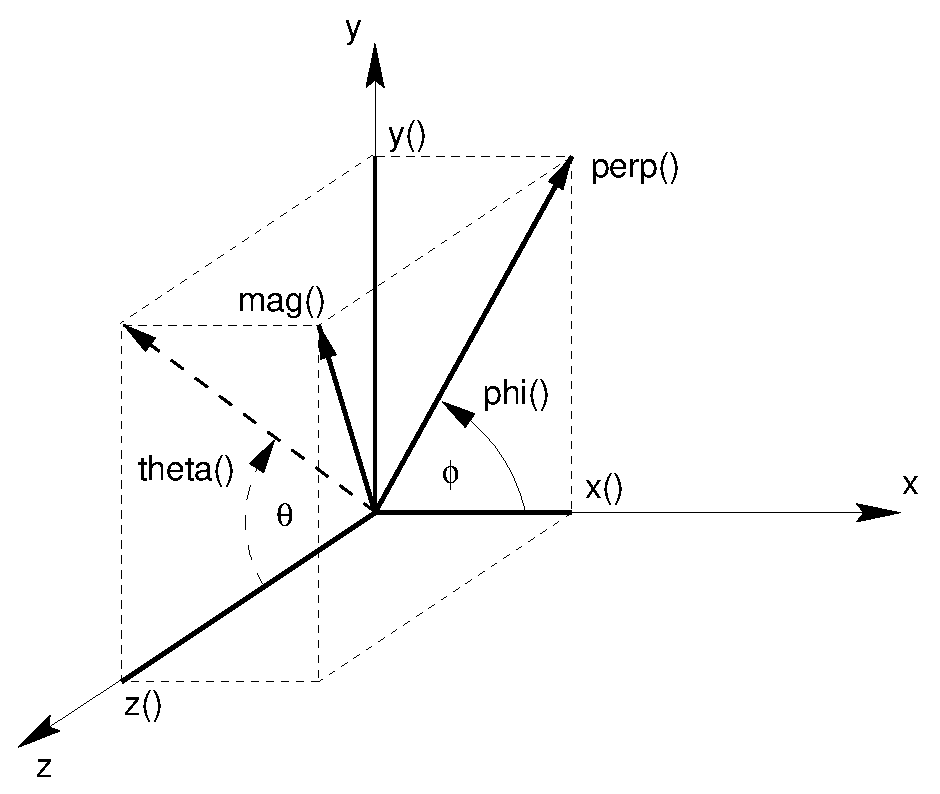
\includegraphics[width=0.65\textwidth]{vec3.eps}
        \caption{Components of three vector: $x,y,z$ - basic components,
            $\theta$ - azimuth angle, $\phi$ - polar angle, mag =
            $\sqrt{x^2+y^2+z^2}$ - magnitude, perp = $\sqrt{x^2+y^2}$
            - transverse component.}
        \label{fig:StThreeVector}
    \end{center}    
\end{figure}

\begin{Entry}
\item[Summary]
    StThreeVector is a templated general 3-vector class defining
    vectors in three dimension (see Fig.~\ref{fig:StThreeVector}).

\item[Synopsis]
    \verb+#include "StThreeVector.hh"+ \\
    \verb+template<class T> StThreeVector;+
    
    
\item[Description]   
    
    This class defines a general 3-vector which can be used to
    represent space points and 3-momenta.  It has a large set of
    member functions, member operators and associated global operators
    which allow to multiply, subtract and add vectors with other
    vectors or scalar variables, calculate cross products and angles
    between vectors, and much more. Once defined its coordinates can
    be obtained in Cartesian, cylindrical and spherical
    representation.  Its interface is essentially the same as
    \comp{ThreeVector} in CLHEP \index{CLHEP} with two significant differences:
    (i) it is templated vector and (ii) it is a concrete class, i.e.
    it is not derived from any other class.  It offers essentially the
    same functionality as the CLHEP version but is more flexible in
    terms of precision and storage optimisation; i.e. in order to
    minimize for memory and storage volume a \comp{StThreeVector}'s
    with type argument \comp{float} can be used but easily
    transformed into a double precision version for computation when
    higher accuracy is needed.  In addition to the CLHEP version there
    are a few member functions added which are useful in the context
    of Heavy-Ion Physics such as \comp{pseudoRapidity()}.

    The template argument is used to define the type associated with
    the x, y, z components. This argument must be one of the floating
    point number data types available in the C++ language, either
    \comp{float}, \comp{double}, or \comp{long double}. The
    default type is \comp{double}.
    
    Please note that \comp{StThreeVector} is {\em not} virtual. This
    is a compromise in order to minimize the storage size, i.e. to
    avoid the additional ballast of the virtual table pointer.
\item[Persistence]
    None

\item[Related Classes]
    Class {\bf StLorentzVector} \index{StLorentzVector}
    is derived from StThreeVector
    defining a 4-dimensional Lorentz vector. 

\item[Public\\ Constructors]
    \verb+StThreeVector<T>();+ \\
    Constructs a 3-vector with all components initialized to 0.
    
    \verb+StThreeVector<T>(T x, T y, T z);+ \\
    Constructs a 3-vector with given components x, y and z.
    
    \verb+template<class X>+\\
    \verb+StThreeVector<T>(const X *avec)+\\
    Constructs a 3-vector from a given array \comp{avec} of type
    X (usually \comp{float} or \comp{double}).
    This is especially useful when a C-style array has to
    be transformed into a StThreeVector. 
    No checks on the array bounderies can be made.
    It is up to the user to make sure that the array
    has the correct size.
    
    \verb+template<class X>+\\
    \verb+StThreeVector<T>(const StThreeVector<X> &vec)+\\
    Copy constructor.
    Constructs a 3-vector with the content of \comp{vec}.
    Note that \comp{vec} can be an object with different
    template arguments then self, i.e.~one can instantiate
    a vector of type \comp{double} with an vector of type
    \comp{float} and vice versa.   
    
\item[Public Member\\ Operators]
    \verb+template<class X>+\\
    \verb+StThreeVector<T>+\\
    \verb+operator= (const StThreeVector<X> &vec);+ \\
    Assignment operator. Replaces the content of self with the content of \comp{vec}.
    Note that \comp{vec} can be an object with different
    template arguments then self, i.e.~one can assign
    a vector of type \comp{double} to a vector of type
    \comp{float} and vice versa.  
    
    \verb+T& operator() (size_t i);+\\
    \verb+T operator() (size_t i) const;+\\    
    Returns components by index. The first version can be used also as
    lvalue.  Note that the first index (the x-component) has index 0.
    The result for indices $> 2$ is platform dependent. If the
    compiler supports exception handling an \comp{out\_of\_range}
    exception is thrown.
    
    \verb+T& operator[] (size_t i);+\\
    \verb+T operator[] (size_t i) const;+\\
    Same as \comp{operator()} above.

    \verb+StThreeVector<T> operator- ();+\\
    Unary minus. Returns copy of self with all components negated.
    
    \verb#StThreeVector<T> operator+ ();#\\
    Unary plus. Returns copy of self.
    
    \verb+StThreeVector<T>&+\\
    \verb+operator*= (double c);+\\
    Returns self multiplied by scalar \comp{c}.
    
    \verb+StThreeVector<T>&+\\
    \verb+operator/= (double c);+\\
    Returns self divided by scalar \comp{c}.
    
    \verb+template<class X>+\\
    \verb+bool+\\
    \verb+operator== (const StThreeVector<X>& vec);+\\
    Equality check. Returns \comp{true} if self equals
    \comp{vec} else \comp{false}.
    
    \verb+template<class X>+\\
    \verb+bool+\\
    \verb+operator!= (const StThreeVector<X>& vec);+\\
    Inequality check. Returns \comp{true} if self is not equal to
    \comp{vec} else \comp{false}.
    

\item[Public Member\\ Functions]
    \verb+void setX(T x);+\\
    Set the x-component in Cartesian coordinate system.
    
    \verb+void setY(T y);+\\
    Set the y-component in Cartesian coordinate system.
    
    \verb+void setZ(T z);+\\
    Set the z-component in Cartesian coordinate system.

    \verb+void setPhi(T ph);+\\
    Set the azimuthal angle in spherical coordinate system.

    \verb+void setTheta(T ph);+\\
    Set the polar angle in spherical coordinate system.

    \verb+void setMag(T r);+\\
    Set the magnitude of the vector keeping the polar and azimuthal
    angles constant.

    \verb+void setMagnitude(T r);+\\
    Set the magnitude of the vector keeping the polar and azimuthal
    angles constant.
    
    \verb+T x() const;+\\
    Returns the x-component in Cartesian coordinate system.
    
    \verb+T y() const;+\\
    Returns the y-component in Cartesian coordinate system.
    
    \verb+T z() const;+\\
    Returns the z-component in Cartesian coordinate system.
    
    \verb+T phi() const;+\\
    Returns the azimuth angle.
    
    \verb+T theta() const;+\\
    Returns the polar angle.
    
    \verb+T cosTheta() const;+\\
    Returns the cosine of the polar angle.
    
    \verb+T mag2() const;+\\
    Returns the magnitude squared of self (r$^2$ in a spherical coordinate system).
    
    \verb+T mag() const;+\\
    Returns the magnitude of self (r in a spherical coordinate system).
    Note that the same value can be obtained using the overloaded
    \comp{abs()} function (see below). \index{abs}
    
    \verb+T perp2() const;+\\
    Returns the transverse component squared
    (R$^2$ in cylindrical coordinate system).
    
    \verb+T perp() const;+\\
    Returns the transverse component
    (R in cylindrical coordinate system). 
    
    \verb+T pseudoRapidity() const;+\\
    Returns the pseudo-rapidity, i.e.~$-\ln(\tan \theta/2)$ of the
    vector. Note that this value is only valid under the assumptions
    that the vector origins from the center of the referring
    reference frame. Be also aware that this member function is
    {\em not} present in the CLHEP ThreeVector class.\index{CLHEP}
    
    \verb+StThreeVector<T> unit() const;+\\
    Returns a unit vector parallel to self.

    \verb+T massHypothesis(T mass) const;+\\
    Calculates what the energy component of a 4-vector
    should be given a mass.  Returns:
    \begin{equation*}
      \sqrt{(*this)^{2} + (mass)^{2}}
    \end{equation*}
    Note this function is not provided in CLHEP.
    
    \verb+StThreeVector<T> orthogonal() const;+\\
    Returns a vector orthogonal to self.  The use of this
    member function is discouraged as the user should
    use the dot and cross products to produce such an
    object.

    \verb+void rotateX(T angle);+\\
    Rotates a vector about the $\hat{x}$ axis according to a right-handed
    coordinate system by an angle specified by \texttt{angle}.

    \verb+void rotateY(T angle);+\\
    Rotates a vector about the $\hat{y}$ axis according to a right-handed
    coordinate system by an angle specified by \texttt{angle}.

    \verb+void rotateZ(T angle);+\\
    Rotates a vector about the $\hat{z}$ axis according to a right-handed
    coordinate system by an angle specified by \texttt{angle}.

    \comp{Note:} No provision to rotate a vector about an arbitrary axis
    is provided in \comp{StThreeVector} as in CLHEP because it is much
    more neatly done by a matrix or rotation class and this would result
    in an additional dependency in \comp{StThreeVector}.  In order
    to do such a rotation, see \comp{StRotation}.\label{StRotation}
    
    \verb+template<class X>+\\
    \verb+T angle(const StThreeVector<X>& vec) const;+\\
    Returns the angle between self and \comp{vec}.
    %, i.e.~$\arccos[\vec{a} \vec{b}/(|\vec{a}| |\vec{b}|)]$
    
    \verb+template<class X>+\\
    \verb+T dot(const StThreeVector<X>& vec) const;+\\
    Returns the scalar product of self and \comp{vec}.
    
    \verb+template<class X>+\\
    \verb+StThreeVector<T>+\\
    \verb+cross(const StThreeVector<X>& vec) const;+\\
    Returns the cross product of self and \comp{vec}.
    
\item[Global Functions]
    \verb+template<class T>+\\
    \verb+T abs(const StThreeVector<T>& vec);+\\ \index{abs}
    Returns the magnitude of \comp{vec}. Same as
    \verb+vec->mag()+.
    Be also aware that this feature is {\em not} provided by
    the CLHEP.\index{CLHEP}
    
    \verb+template<class T, class X>+\\
    \verb+StThreeVector<T>+\\
    \verb+cross_product(const StThreeVector<T>& v1,+\\
    \verb+              const StThreeVector<X>& v2);+\\
    Returns the cross product of \comp{v1} and \comp{v2}.
    The type of the returned vector is determined by the type
    argument of the first vector \comp{v1}. Note that the
    name was chosen for compatibility with the STL.
    
\item[Global Operators]
    \verb+template<class T, class X>+\\
    \verb+StThreeVector<T>+\\
    \verb#operator+ (const StThreeVector<T>& v1,#\\
    \verb+           const StThreeVector<X>& v2);+\\
    Returns the sum of \comp{v1} and \comp{v2}.
    The type of the returned vector is determined by the type
    argument of the first vector \comp{v1}.
    
    \verb+template<class T, class X>+\\
    \verb+StThreeVector<T>+\\
    \verb+operator- (const StThreeVector<T>& v1,+\\
    \verb+           const StThreeVector<X>& v2);+\\
    Returns the \comp{v1} minus \comp{v2}.
    The type of the returned vector is determined by the type
    argument of the first vector \comp{v1}.
     
    \verb+template<class T, class X>+\\
    \verb+T operator* (const StThreeVector<T>& v1,+\\
    \verb+             const StThreeVector<X>& v2);+\\
    Returns the scalar product of \comp{v1} and \comp{v2}.
    The type of the returned value is determined by the type
    argument of the first vector \comp{v1}.
    
    \verb+template<class T>+\\
    \verb+StThreeVector<T>+\\
    \verb+operator* (const StThreeVector<T>& vec,+\\
    \verb+           double c);+\\
    Returns vector \comp{vec} multiplied by scalar c.
    
    \verb+template<class T>+\\
    \verb+StThreeVector<T>+\\
    \verb+operator* (double c,+\\
    \verb+           const StThreeVector<T>& vec);+\\
    Returns vector \comp{vec} multiplied by scalar c.
    
    \verb+template<class T, class X>+\\
    \verb+StThreeVector<T>+\\
    \verb+operator/ (const StThreeVector<T>& vec,+\\
    \verb+           X c);+\\
    Returns vector \comp{vec} divided by scalar c.

    \verb+template<class T>+\\
    \verb+ostream&+\\
    \verb+operator<< (ostream& os,+\\
    \verb+           const StThreeVector<T>& vec);+\\
    Prints vector \comp{vec} to output stream \comp{os}.
    
    \verb+template<class T>+\\
    \verb+istream&+\\
    \verb+operator>> (istream& is,+\\
    \verb+           StThreeVector<T>& vec);+\\
    Reads vector \comp{vec} from input stream \comp{is}.
    Be also aware that this operator is {\em not} provided by
    the CLHEP ThreeVector class.\index{CLHEP}

\item[Examples]
{\footnotesize
\begin{verbatim}
#include "StThreeVector.hh"

int main()
{
    StThreeVector<double>  a;
    StThreeVector<double>  b(1,2,3);
    StThreeVector<float>   c(b);

    cout << "b = " << b << endl;
    cout << "c = " << c << endl;

    // add two vectors
    a = b+c;
    cout << "a = b+c = " << a << endl;

    // check for inequality
    if (a != b*2) {
        cerr << "Oops ..." << endl;
        return 1;
    }

    // modify components of vector c
    c.setX(4);
    c.setY(7);
    cout << "c = " << c << endl;

    // inner product
    double d = a*c;
    cout << "a*c = " << d << endl;

    // angle
    cout << "angle(a,c) = "
         << a.angle(c) << endl;

    // cross product
    cout << "a X c = "
         << a.cross(c) << endl;
    
    // pseudo rapidity
    cout << "pseudo rapidity(c) = "
         << c.pseudoRapidity() << endl;
    
    return 0;
}
\end{verbatim}

{\bf Programs Output:}

\begin{verbatim}
b = (1, 2, 3)
c = (1, 2, 3)
a = b+c = (2, 4, 6)
c = (4, 7, 3)
a*c = 54
angle(a,c) = 0.575631
a X c = (-30, 18, -2)
pseudo rapidity(c) = 0.364012
\end{verbatim}
}
\end{Entry}

\clearpage

%%%%%%%%%%%%%%%%%%%%%%%%%%%%%%%%%%%%%%%%%%%%%%%%%%%%%%%%%%%%%%%%%%%%
%
%    Reference: StThreeVectorD
%
%%%%%%%%%%%%%%%%%%%%%%%%%%%%%%%%%%%%%%%%%%%%%%%%%%%%%%%%%%%%%%%%%%%%
\subsection{StThreeVectorD \index{StThreeVectorD|textbf}}
\begin{Entry}
\item[Summary]
    StThreeVectorD is a non-template version of \verb+StThreeVector<double>+
    (see \ref{StThreeVector}). The code does not contain templates nor
    does it make use of the Standard C++ library. All data member are of
    type \texttt{double}.
    
\item[Synopsis]
    \verb+#include "StThreeVectorD.hh"+ \\
    \verb+StThreeVectorD;+
    
    
\item[Description]       
    The member functions, operators and non-member functions are identical
    to those of StThreeVector but might be slightly slower in execution speed
    since the inline mechanism cannot be used as extensive as for the template
    version. Operations can be mixed with the non-template single precision version
    \texttt{StThreeVectorF} but not with any instance of \verb+StThreeVector<T>+.
    The templated version should be preferred where possible.
    
\item[Related Classes]
    StThreeVectorD inherits from TObject \index{TObject}
    if the SCL was compiled with the \name{\_\_ROOT\_\_} flag set.

\item[Persistence]
    Within the ROOT framework.

\end{Entry}

%%%%%%%%%%%%%%%%%%%%%%%%%%%%%%%%%%%%%%%%%%%%%%%%%%%%%%%%%%%%%%%%%%%%
%
%    Reference: StThreeVectorF
%
%%%%%%%%%%%%%%%%%%%%%%%%%%%%%%%%%%%%%%%%%%%%%%%%%%%%%%%%%%%%%%%%%%%%
\subsection{StThreeVectorF \index{StThreeVectorF|textbf}}
\begin{Entry}
\item[Summary]
    StThreeVectorF is a non-template version of \verb+StThreeVector<float>+
    (see \ref{StThreeVector}). The code does not contain templates nor
    does it make use of the Standard C++ library. All data member are of
    type \texttt{float}.
    
\item[Synopsis]
    \verb+#include "StThreeVectorF.hh"+ \\
    \verb+StThreeVectorF;+
    
\item[Description]       
    The member functions, operators and non-member functions are identical
    to those of StThreeVector but might be slightly slower in execution speed
    since the inline mechanism cannot be used as extensive as for the template
    version. Operations can be mixed with the non-template double precision version
    \texttt{StThreeVectorD} but not with any instance of \verb+StThreeVector<T>+.
    The templated version should be preferred where possible.

\item[Related Classes]
    StThreeVectorF inherits from TObject \index{TObject}
    if the SCL was compiled with the \name{\_\_ROOT\_\_} flag set.

\item[Persistence]
    Within the ROOT framework.

\end{Entry}

\clearpage

%%%%%%%%%%%%%%%%%%%%%%%%%%%%%%%%%%%%%%%%%%%%%%%%%%%%%%%%%%%%%%%%%%%%
%
%    Reference: StTimer
%
%%%%%%%%%%%%%%%%%%%%%%%%%%%%%%%%%%%%%%%%%%%%%%%%%%%%%%%%%%%%%%%%%%%%
\subsection{StTimer \index{StTimer|textbf}}
\index{timer}
\index{CPU timer}
\begin{Entry}
\item[Summary]
    CPU timer
    
\item[Synopsis]
    \verb+#include "StTimer.hh"+ \\
    \verb+StTimer timer;+
    
\item[Description]    
    This class can measure elapsed CPU (user) time. The timer has two
    states: running and stopped. The timer measures the total amount
    of time spent in the "running" state since it was either
    constructed or reset.
    
    The timer is put into the "running" state by calling member
    function \comp{start()}. It is put into the "stopped" state by
    calling \comp{stop()}.
    
    StTimer uses the system-dpendent function \comp{clock()} which
    returns the number of "ticks" since it was first called. As a
    result, StTimer will not be able to measure intervals longer than
    some system-dependent value. (For instance, on several common UNIX
    systems, this value is just under 36 minutes.)
    
    The resolution of the timer is given by the number of "ticks" per
    second.  This value is system dependent and can be checked with
    the \comp{resolution()} member function. Make sure that the CPU time
    between the start and stop of the timer is significantly larger
    than the resolution.

    N.B. The interface of this class and its functionality were adapted
    from the tools.h++ class library from RogueWave.
    
\item[Related Classes]
    None
    
\item[Persistence]
    None
    
\item[Public\\ Constructors]
    \verb+StTimer();+ \\
    Constructs a new timer. The timer will not start
    running until until \comp{start()} is called.

\item[Public Member\\ Functions]
    \verb+double resolution() const+\\
    Returns the minimal amount of time in seconds which can be
    measured by the timer. This value is system dependent.
    Typical values range from 10 $\mu$s to 10 ms.
    
    \verb+double elapsedTime() const+\\
    Returns the amount of (CPU) time that has accumulated while
    the timer was in the running state.
 
    \verb+void reset()+\\
    Resets (and stops) the timer.
 
    \verb+void start()+\\
    Puts the timer in the "running" state. Time accumulates while
    in this state.

    \verb+void stop()+\\
    Puts the timer in the "stopped" state. Time will not accumulate
    while in this state.

\item[Example]
{\footnotesize
\begin{verbatim}
#include "StTimer.hh"
#include <time.h>
#include <iostream.h>
#include <math.h>

int main()
{   
    StTimer timer, totalTimer;
    
    totalTimer.start();
    timer.start();
    
    // Spend 5 busy sec.
    time_t begin = time(0);
    time_t now = begin;
    while (now - begin < 5) now = time(0);
    
    timer.stop();
    
    cout << "Test 1:" << endl;
    cout << "This test should require less than 5 sec CPU time. \n"
         << "The exact amount depends strongly on the system." << endl;
    cout << "The measured elapsed CPU time is: "
         << timer.elapsedTime() << " sec\n" << endl;
    
    timer.reset();
    timer.start();
    
    const size_t NumSqrt = 1000000;
    double x;
    for (int i=0; i<NumSqrt; i++) x = sqrt(double(i));
    
    timer.stop();
    
    cout << "Test 2:" << endl;
    cout << "The CPU time to calculate " << NumSqrt
         << " square roots is: "
         << timer.elapsedTime() << " sec\n" << endl;
    
    cout << "The total amount of CPU seconds used \n"
         << "to execute this program is: ";
    totalTimer.stop();
    cout << totalTimer.elapsedTime() << " sec." << endl;
    
    return 0;
}
\end{verbatim}

{\bf Programs Output:}

\begin{verbatim}
Test 1:
This test should require less than 5 sec CPU time. 
The exact amount depends strongly on the system.
The measured elapsed CPU time is: 4.81 sec

Test 2:
The CPU time to calculate 1000000 square roots is: 0.25 sec

The total amount of CPU seconds used 
to execute this program is: 5.06 sec.
\end{verbatim}
}

\end{Entry}

\clearpage

%%%%%%%%%%%%%%%%%%%%%%%%%%%%%%%%%%%%%%%%%%%%%%%%%%%%%%%%%%%%%%%%%%%%
%
%    Reference: Random
%
%%%%%%%%%%%%%%%%%%%%%%%%%%%%%%%%%%%%%%%%%%%%%%%%%%%%%%%%%%%%%%%%%%%%
\subsection{Random \index{Random|textbf}} \label{Random}
\begin{Entry}
\item[Summary]
    Random provides a mechanism to generate pseudo-random numbers in
    a variety of distributions.  Provided are several engines
    that provide seeds to classes that are able to generate random
    numbers according to several pre-determined distribution.
    
\item[Synopsis]
    \verb+#include "Random.hh"+\\
    \verb+// At least one engine+\\
    \verb+#include "JamesRandom.h"   // The engine used by default+\\
    \verb+#include "RanecuEngine.h"+\\
    \verb+#include "RanluxEngine.h"+\\
    \verb+#include "DRand48Engine.h"+\\
    \verb+#include "RandEngine.h"+\\
    \verb+// And a type of distribution+\\
    \verb+#include "RandFlat.h"+\\
    \verb+#include "RandPoisson.h"+\\
    \verb+#include "RandExponential.h"+\\
    \verb+#include "RandGauss.h"+\\
    \verb+#include "RandBreitWigner.h"+\\ \\
    \verb+// Note: all Random header files are contained in:+\\
    \verb+#include "Randomize.h"+\\
    
\item[Description]   

  Random consists of a series of classes that provide mechanisms to
  generate pseudo-random numbers according to one of five pre-determined
  distributions:
  \begin{itemize}
   \item Flat
   \item Poissonian
   \item Exponential
   \item Gaussian
   \item Breit-Wigner
  \end{itemize}

  In order to generate a random number according to these distributions
  a pseudo-random number engine must be provided.  These engines
  utilize either a predefined (static) seed table \index{seed table}
  or a seed given by the user and one of several prescriptions
  to generate a pseudo-random
  number in a flat distribution.  These numbers are then used to generate
  a random number based on a characteristic distribution.
  
  It should be noted that these classes are nearly exact copies of those
  used in CLHEP\index{CLHEP} (hence the lack of the ``{\bf St}'' prefix)
  adapted for use in the STAR Class Library.  Member functions that
  are not contained within CLHEP are specified as such.
  
  \begin{itemize}
    \item Arrays passed to member functions should be replaced with
      STL containers.
    \item A reduction of member functions by using default values for
      arguments.
    \item \ldots
  \end{itemize}
  
  There exists two classes which define the two different components
  of the category:
  \begin{itemize}
    \item \comp{RandomEngine.h} contains an abstract class {\em HepRandomEngine}
      which defines the interface for all random engines.
    \item \comp{Random.h} defines  {\em HepRandom} which is a base class
      from which all distribution classes inherit.  It defines both
      static and non-static interfaces as well as the default engine
      generator (i.e.~HepJamesRandom).
    \end{itemize}
    
\item[Persistence]
    None

\item[Related Classes]
  {\bf The Engines:}
  
    Class {\em HepRandomEngine} (contained in \comp{RandomEngine.h}) is a purely
    abstract class which defines the user interface for all engines:

     \verb+double flat();+\\
     Returns a pseudo-random number from a flat distribution
     in the interval (0,1).

     \verb+void flatArray(const int size, double* vec);+\\
     Fills an array \comp{vec} of size \comp{size} with random
     numbers derived from a flat distribution.

     \verb+void flatArray(vector<double>& vec);+\\
     Fills a vector \comp{vec} with random
     numbers derived from a flat distribution.  This is
     not supported by CLHEP.
     
     \verb+void setSeed(long seed, int init);+\\
     (Re)-initialize the status of the algorithm with a user specified
     seed.
     
     \verb+void setSeeds(const long* seeds, int init);+\\
     (Re)initializes the generator with a zero terminated list of seeds.
     
     \verb+void saveStatus() const;+\\
     Saves the current status of the instantiated engine
     in a file (\comp{.conf}).  This provides a mechanism
     to recover a series of random numbers.

     \verb+void restoreStatus();+ \\
     Reads from a file (specific to the instantiated engine in use)
     and restore the last saved engine configuration.  For use with
     \comp{saveStatus()}.

     \verb+showStatus() const;+\\
     Dumps the current engine status to \comp{stdout}.

     \verb+long getSeed() const;+\\
     Returns the current seed from the current generator.

     \verb+const long* getSeeds() const;+\\
     Returns the current array of seeds from the current generator.

     \verb+void getTableSeeds(long* seeds, int index) const;+\\
     Returns the seed values stored in the global \comp{seedTable}
     that is located at the \comp{index} position.

     {\em The Specific Engines:}
     
     \begin{description}
       \item {\bf HepJamesRandom} implements the algorithm of
       Marsaglia-Zaman RANMAR which is described in
       {\em F.  James, Comp. Phys. Comm. {\bf 60} (1990) 329}.  It is a
       component of the MATHLIB HEP library for pseudo-random
       number generation.  This is the default random engine invoked
       by each distribution unless the user specifies a different one.

       \item {\bf DRand48Engine} uses \comp{drand48()}
         and \comp{srand48()} functions from the C standard library
         to implement the basic \comp{flat()} basic distribution and
         for setting seeds.  Note that this file is part of the
         Geant4 \index{GEANT4} simulation toolkit.

       \item {\bf RandEngine} uses the \comp{rand()} and \comp{srand()}
         functions from the C standard library to implement the \comp{flat()}
         basic distribution and for setting seeds.  Note that this file is
         part of Geant4 simulation toolkit.

       \item {\bf RanecuEngine} is an algorithm that is part of the
         MATHLIB HEP library.  Seeds are taken from a seed table
         and given an index.  The \comp{getSeed()} member function
         returns the current index of the seed table, while the
         \comp{getSeeds()} member function returns a pointer to the
         local table of seeds at the current index.  Note that this file
         is part of Geant4 simulation toolkit.

       \item {\bf RanluxEngine} is an algorithm originally implemented
         in FORTRAN by Fred James as part of the MATHLIB HEP
         library.  The initialisation is carried out using a
         Multiplicative Congruential generator using formula constants
         of L'Ecuyer as described in {\em F. James, Comp. Phys. Comm. 60 (1990) 329}.
         Note that this file is part of Geant4 simulation toolkit.
     \end{description}

  {\bf The Distributions:}
  
     Class {\em HepRandom} contained in \comp{Random.h} is a base class
     from which all distribution
     classes inherit.  An object of this class is instantiated by
     default within the HEP Random module.  An instantiated {\em HepJamesRandom}
     engine is used as a default algorithm for pseudo-random number
     generation.  HepRandom defines a static private data member
     \comp{theGenerator} and a set of static inlined methods to
     manipulate it. By means of \comp{theGenerator} the user can:
     \begin{itemize}
        \item change the underlying engine algorithm.
        \item get and set the seeds.
        \item use any kind of defined random distribution.
      \end{itemize}
      {\bf Note:} Distribution classes inherit from {\em HepRandom} and define
      {\bf both} static and non-static interfaces.

\item[Public\\ Constructors]
      \verb+HepRandom();+\\
      Contructor without a seed uses the default engine (i.e.~{\em HepJamesRandom}).

      \verb+HepRandom(long seed);+\\
      Contructor with a seed specified by the user which uses the
      default engine (i.e.~{\em HepJamesRandom}).

      \verb+HepRandom(HepRandomEngine& algorithm);+\\
       Constructor with a user specified generating engine.
       When algorithm is passed by reference, it will {\bf not}
       be deleted by the {\em HepRandom} destructor.

      \verb+HepRandom(HepRandomEngine* algorithm);+\\
      Constructor with a user specified generating engine. When
      algorithm is passed by pointer, it will be deleted by the
      HepRandom destructor.
  
\item[Public Member\\ Functions]

    \verb+double flat();+\\
    Returns the flat value in the interval (0,1).

    \verb+double flat (HepRandomEngine* theNewEngine);+\\
    Returns a flat value in the interval (0,1)
    where \comp{theNewEngine} is used as the Random Engine.

    \verb+void flatArray(const int size, double* vect);+\\
    Fills the array \comp{vect} of size \comp{size}
    with flat random values.  Please note that when STL containers are
    implemented the size will no longer be a required argument.

    \verb+void flatArray(HepRandomEngine* theNewEngine,+\\ 
    \verb+                    const int size, double* vect);+\\
    Fills the array \comp{vect} of size \comp{size} with flat
    random values, given a user specified Random Engine.
    Please note that when STL containers are implemented the size
    will no longer be a required argument.

\item[Static Member\\ Functions]

    \verb+void setTheSeed(long seed, int lux=3);+\\
    Specifies the seed for the engine.

    \verb+long getTheSeed();+\\
    Returns the static definition for the seed.

    \verb+void setTheSeeds(const long* seeds, int aux=-1);+\\
    Specifies a table of seeds for the engine to use.

    \verb+const long* getTheSeeds();+\\
    Returns the table of seeds currently in use.

    \verb+void getTheTableSeeds (long* seeds, int index);+\\
    Returns the table of seeds starting from a specific \comp{index}
    position.

    \verb+HepRandom* getTheGenerator();+\\
    Return a pointer to the current static generator.

    \verb+void setTheEngine (HepRandomEngine* theNewEngine);+\\
    Specifies the engine to be used in the pseudo-random number generation.

    \verb+HepRandomEngine* getTheEngine();+\\
    Returns a pointer to the current engine in use.

    \verb+void saveEngineStatus();+\\
    Saves the current engine status in a \comp{.conf} file.
    
    \verb+void restoreEngineStatus();+\\
    Restores the status of an engine to that specified in
    a \comp{.conf} file.  In the absence of such a file,
    nothing is done.

    \verb+void showEngineStatus();+\\
    Prints the status of the random engine to \comp{stdout}.
        
\item[Public Member\\ Operators]
    \verb+double operator()();+\\
    Generates a single random number.
  
    The Specific Distribution classes include functionality that is specific
    to their own properties:
    
    \begin{description}
      \item \underline{\bf RandFlat} \index{RandFlat} defines methods for generating flat random numbers
        which can be either \comp{integer} or \comp{double} precision.
        It also provides static methods to fill arrays of a specified size.
    \end{description}
    
\item[Public Member\\ Constructors]
  
    \verb+RandFlat(HepRandomEngine& anEngine);+\\
    Constructor instantiates a \comp{RandFlat} distribution
    object defining a local engine (by reference) for it.  The
    corresponding engine object will {\bf not} be deleted by the
    \comp{RandFlat} destructor.
     
    \verb+RandFlat(HepRandomEngine* anEngine);+\\
    Constructor instantiates a \comp{RandFlat} distribution
    object defining a local engine (by pointer) for it.
    The corresponding engine object will be deleted by the
    \comp{RandFlat} destructor.

\item[Public Static Member\\ Functions]
  
    Static methods to generate random values using the static generator
    are provided:

    \verb+double shoot();+\\
    Returns a double precision number from a flat distribution
    in the interval (0,1).
    
    \verb+shoot(double width);+\\
    Returns a double precision number from a flat distribution
    in the interval (0,width).
    
    \verb+double shoot(double a, double b);+\\
    Returns a double precision number from a flat distribution
    in the interval (a,b).

    \verb+long shootInt(long n);+\\
    Returns an integer number from a flat distribution
    in the interval (0,n).
    
    \verb+long shootInt(long m, long n);+\\
    Returns an integer number from a flat distribution
    in the interval (m,n).
    
    \verb+int shootBit();+\\
    Returns either 0 or 1 according to a flat distribution.
    
    \verb+void shootArray(const int size, double* vect);+\\
    Fills an array \comp{vect} of size \comp{size} with double
    precision numbers in the interval (0,1).

    \verb+void shootArray(vector<double>& vec);+\\
    Fills a vector \comp{vec} with double
    precision numbers in the interval (0,1).
    This is not supported in CLHEP.

    \verb+void shootArray(const int size, double* vect,+\\
    \verb+                          double lx, double dx);+\\
    Fills an array \comp{vect} of size \comp{size} with double
    precision numbers in the interval (lx,dx).

    \verb+void shootArray(vector<double>& vec, double lx, double dx);+\\
    Fills a vector \comp{vec} with double
    precision numbers in the interval (lx,dx).
    This is not supported in CLHEP.
    
    \verb+double shoot(HepRandomEngine* anEngine);+\\
    Returns a double precision number in the interval (0,1)
    where the engine is specified by the user.
    
    \verb+double shoot(HepRandomEngine* anEngine,+\\
    \verb+                              double width);+\\
    Returns a double precision number in the interval (0,width)
    where the engine is specified by the user.
    
    \verb+double shoot(HepRandomEngine* anEngine,+\\
    \verb+                            double a, double b);+\\
    Returns a double precision number in the interval (a,b)
    where the engine is specified by the user.
    
    \verb+long shootInt(HepRandomEngine* anEngine, long n);+\\
    Returns an integer number in the interval (0,n)
    where the engine is specified by the user.
    
    \verb+long shootInt(HepRandomEngine* anEngine,+\\
    \verb+                              long m, long n);+\\
    Returns an integer number in the interval (m,n)
    where the engine is specified by the user.
    
    \verb+ont shootBit(HepRandomEngine* anEngine);+\\
    Returns 0 or 1 where the engine is specified.
    
    \verb+void shootArray(HepRandomEngine* anEngine,+\\
    \verb+                  const int size, double* vect);+\\
    Fills an array \comp{vect} of size \comp{size} with double
    precision numbers in the interval (0,1) where the engine is
    specified.

    \verb+void shootArray(HepRandomEngine* anEngine,+\\
    \verb+                         vector<double>& vec);+\\
    Fills a vector \comp{vec} with double
    precision numbers in the interval (0,1) where the engine is
    specified.  This is not supported in CLHEP.
    
   \verb+void shootArray(HepRandomEngine* anEngine,+\\ 
   \verb+              const int size, double* vect,+\\
   \verb+                      double lx, double dx);+\\
   Fills an array \comp{vect} of size \comp{size} with double
   precision numbers in the interval (lx,dx) where the engine is
   specified.

   \verb+void shootArray(HepRandomEngine* anEngine,+\\ 
   \verb+     vector<double>& vec, double lx, double dx);+\\
   Fills a vector \comp{vect} with double
   precision numbers in the interval (lx,dx) where the engine is
   specified.  This is not supported in CLHEP.
   
  The following methods use the localEngine to shoot random values,
  by-passing the static generator.

   \verb+double fire();+\\
   Returns a double precision number in the interval (0,1).
  
   \verb+double fire(double width);+\\
   Returns a double precision number in the interval (0,width).
   
   \verb+double fire(double a, double b);+\\
   Returns a double precision number in the interval (a,b).

   \verb+long fireInt(long n);+\\
   Returns an integer number in the interval (0,n).
  
   \verb+long fireInt(long m, long n);+\\
   Returns an integer number in the interval (m,n).

   \verb+int fireBit();+\\
   Returns either 0 or 1.
  
   \verb+void fireArray(const int size, double* vect);+\\
   Fills an array \comp{vect} of size \comp{size} with double
   precision numbers in the interval (0,1).

   \verb+void fireArray(vector<double>& vec);+\\
   Fills a vector \comp{vec} with double
   precision numbers in the interval (0,1).
   This is not supported in CLHEP.
   
   \verb+void fireArray(const int size, double* vect,+\\
   \verb+                          double lx, double dx);+\\
   Fills an array \comp{vect} of size \comp{size} with double
   precision numbers in the interval (lx,dx)

   \verb+void fireArray(vector<double>& vec, double lx, double dx);+\\
   Fills a vector \comp{vec} with double
   precision numbers in the interval (lx,dx)
   This is not supported in CLHEP.
   
   \begin{description}
     \item \underline{\bf RandGauss} \index{RandGauss} defines methods for generating random
      numbers which are distributed in a Gaussian manner:
   \end{description}
   
\item[Public Member\\ Constructors]

   \verb+RandGauss(HepRandomEngine& anEngine);+\\
   Constructor to instantiate a Gaussian random number generator
   where \comp{anEngine} is the generating engine.  The corresponding
   engine object will {\bf not} be deleted by the \comp{RandGauss} destructor.
   
   \verb+RandGauss(HepRandomEngine* anEngine);+\\
   Constructor to instantiate a Gaussian random number generator
   where \comp{anEngine} is the generating engine.  The corresponding
   engine object will be deleted by the \comp{RandGauss} destructor.
  
\item[Public Static Member\\ Functions]
  
   \verb+double shoot();+\\
   Returns a double precision number from a Gaussian distribution where the
   mean is 0 and standard deviation is 1.
  
   \verb+double shoot(double mean, double stdDev);+\\
   Returns a double precision number from a Gaussian distribution where the
   mean is \comp{mean} and standard deviation is given by
   \comp{stdDev}.

  \verb+void shootArray(const int size, double* vect,+\\
  \verb+         double mean=0.0, double stdDev=1.0);+\\
  Fills an array \comp{vect} of size \comp{size} with double
  precision number from a distribution where the
  mean is \comp{mean} (0 by default) and standard
  deviation is \comp{stdDev} (1 by default).

  \verb+void shootArray(vector<double>& vec,+\\
  \verb+         double mean=0.0, double stdDev=1.0);+\\
  Fills a vector \comp{vec} with double
  precision number from a distribution where the
  mean is \comp{mean} (0 by default) and standard
  deviation is \comp{stdDev} (1 by default).  This is not
  supported in CLHEP.
  
  Static methods to shoot random values using a given engine
  bypassing the static generator are also provided:

  \verb+double shoot(HepRandomEngine* anEngine);+\\
  Returns a double precision number from a Gaussian distribution where the
  mean is 0 and standard deviation is 1
  and the engine is specified by the user.
  
  \verb+double shoot(HepRandomEngine* anEngine,+\\ 
  \verb+                 double mean, double stdDev);+\\
  Returns a double precision number from a Gaussian distribution where the
  mean is \comp{mean} and standard deviation is \comp{stdDev}
  and the engine is specified.

  \verb+void shootArray(HepRandomEngine* anEngine,+\\
  \verb+       const int size,double* vect,+\\ 
  \verb+       double mean=0.0, double stdDev=1.0);+\\
  Fills an array \comp{vect} of size \comp{size} with double precision
  numbers from a Gaussian distribution where the
  mean is \comp{mean} and standard deviation is \comp{stdDev}
  and the engine is specified.

  \verb+void shootArray(HepRandomEngine* anEngine,+\\
  \verb+       vector<double>& vec,+\\ 
  \verb+       double mean=0.0, double stdDev=1.0);+\\
  Fills a vector \comp{vec} with double precision
  numbers from a Gaussian distribution where the
  mean is \comp{mean} and standard deviation is \comp{stdDev}
  and the engine is specified.  This is not supported by CLHEP.
  
  Methods using the local engine to generate random values, bypassing
  the static generator are also provided:

  \verb+double fire();+\\
  Returns a double precision number from a Gaussian distribution where the
  mean is 0 and standard deviation is 1.
  
  \verb+double fire(double mean, double stdDev);+\\
  Returns a double precision number from a Gaussian distribution where the
  mean is \comp{mean} and standard deviation is \comp{stdDev}.
  
  \verb+void fireArray(const int size, double* vect,+\\
  \verb+        double mean=0.0, double stdDev=1.0);+\\
  Fills an array \comp{vect} of size \comp{size} with double
  precision number from a distribution where the
  mean is \comp{mean} (0 by default) and standard
  deviation is \comp{stdDev} (1 by default).

  \verb+void fireArray(vector<double>& vec,+\\
  \verb+        double mean=0.0, double stdDev=1.0);+\\
  Fills a vector \comp{vec} with double
  precision number from a distribution where the
  mean is \comp{mean} (0 by default) and standard
  deviation is \comp{stdDev} (1 by default).  This is not
  supported in CLHEP.
  
  \begin{description}
      \item \underline{\bf RandExponential} \index{RandExponential} defines methods for generating
        random numbers distributed according to an exponential distribution.
  \end{description}
      
\item[Public Member\\ Constructors]

   \verb+RandExponential(HepRandomEngine& anEngine);+\\
   Constructor to instantiate a {\em RandExponential}
   distribution object and specifying a local engine for it.
   The engine passed by reference will {\bf not} be deleted by
   the RandExponential destructor.
   
   \verb+RandExponential(HepRandomEngine* anEngine );+\\
   Constructor to instantiate a {\em RandExponential}
   distribution object and specifying a local engine for it.
   The engine passed by pointer will be deleted by the RandExponential
   destructor.

\item[Public Static Member\\ Functions]

   \verb+double shoot();+\\
   Returns a double precision number from an exponential distribution where the
   mean is 1.
  
   \verb+double shoot(double mean);+\\
   Returns a double precision number from an exponential distribution where the
   mean is specified by \comp{mean}.
  
   \verb+void shootArray(const int size, double* vect,+\\
   \verb+                                double mean=1.0);+\\
   Fills an array \comp{vect} of size \comp{size} from an exponential distribution
   where the mean is specified by \comp{mean} (default is 1).

   \verb+void shootArray(vector<double>& vec, double mean=1.0);+\\
   Fills a vector \comp{vec} from an exponential distribution
   where the mean is specified by \comp{mean} (default is 1).  This
   is not supported in CLHEP.
 
   Static methods to generate random values using a given engine
   bypassing the static generator are also provided.

   \verb+double shoot(HepRandomEngine* anEngine);+\\
   Returns a double precision number from an exponential  distribution where the
   mean is 1 and the engine is specified by \comp{anEngine}.
  
   \verb+double shoot(HepRandomEngine* anEngine,+\\
   \verb+                                double mean);+\\
   Returns a double precision number from an exponential distribution where the
   mean is specified by \comp{mean} and the engine is specified
   by \comp{anEngine}.
  
   \verb+void shootArray(HepRandomEngine* anEngine,+\\
   \verb+const int size, double* vect, double mean=1.0);+\\
   Fills an array \comp{vect} of size \comp{size} from an exponential distribution
   where the mean is specified by \comp{mean} (default is 1) and
   the engine is specified by \comp{anEngine}.

   \verb+void shootArray(HepRandomEngine* anEngine,+\\
   \verb+     vector<double>& vec, double mean=1.0);+\\
   Fills a vector \comp{vec} from an exponential distribution
   where the mean is specified by \comp{mean} (default is 1) and
   the engine is specified by \comp{anEngine}.  This is not supported
   in CLHEP.
   
   Methods using the local Engine to generate random values, bypassing
   the static generator are also provided:

   \verb+double fire();+\\
   Returns a double precision number from an exponential distribution where the
   mean is 1.
  
   \verb+double fire(double mean);+\\
   Returns a double precision number from an exponential distribution where the
   mean is specified by \comp{mean}.

   \verb+void fireArray(const int size, double* vect,+\\
   \verb+                                  double mean=1.0);+\\
   Fills an array \comp{vect} of size \comp{size} from an exponential distribution
   where the mean is specified by \comp{mean} (default is 1).

   \verb+void fireArray(vector<double>& vec, double mean=1.0);+\\
   Fills a vector \comp{vec} from an exponential distribution
   where the mean is specified by \comp{mean} (default is 1).
   This is not supported in CLHEP.

   \begin{description}
     \item \underline{\bf RandPoisson} \index{RandPoisson} defines methods for generation numbers
       according to a Poisson distribution.  The algorithm was taken
       from {\em W. H. Press et al., Numerical Recipes in C, Second Edition}.
   \end{description}
   
\item[Public Member\\ Functions]

    \verb+RandPoisson(HepRandomEngine& anEngine);+\\
    Constructor to instantiate a {\em RandPoisson}
    distribution and specifying a \underline{local} engine for it.
    The engine \comp{anEngine} passed by reference will {\bf not}
    be deleted by the {\em RandPoisson} destructor.
  
    \verb+RandPoisson( HepRandomEngine* anEngine);+\\
    Constructor to instantiate a {\em RandPoisson}
    distribution and specifying a \underline{local} engine for it.
    The engine passed by pointer will be deleted by the {\em RandPoisson}
    destructor.

    Static methods to shoot random values using the static generator
    are provided:

    \verb+long shoot(double mean=1.0);+\\
    Returns an integer from a Poissonian distribution with a mean
    specified by \comp{mean} (default is 1).

    \verb+void shootArray(const int size, long* vect,+\\
    \verb+                               double mean=1.0);+\\
    Fills an integer array \comp{vect} of size \comp{size} from a
    Poissonian distribution with a mean specified by \comp{mean}
    (default is 1).

    \verb+void shootArray(vector<long>& vec, double mean=1.0);+\\
    Fills an integer vector \comp{vec} from a
    Poissonian distribution with a mean specified by \comp{mean}
    (default is 1).  This is not supported by CLHEP.

    Static methods to shoot random values using a given engine
    bypassing the static generator are also provided:

    \verb+long shoot(HepRandomEngine* anEngine,+\\
    \verb+                           double mean=1.0);+\\
    Returns an integer from a Poissonian distribution with a mean
    specified by \comp{mean} (default is 1) and the engine specified
    by \comp{anEngine}.
  
    \verb+void shootArray(HepRandomEngine* anEngine,+\\
    \verb+     const int size, long* vect, double mean=1.0 );+\\
    Fills an integer array \comp{vect} of size \comp{size} from a
    Poissonian distribution with a mean specified by \comp{mean}
    (default is 1) and the engine specified by \comp{anEngine}.

    \verb+void shootArray(HepRandomEngine* anEngine,+\\
    \verb+        vector<long>& vec, double mean=1.0 );+\\
    Fills an integer vector \comp{vec} from a
    Poissonian distribution with a mean specified by \comp{mean}
    (default is 1) and the engine specified by \comp{anEngine}.
    This is not supported in CLHEP.
    
    Methods using the localEngine to shoot random values, bypassing
    the static generator are also provided:

    \verb+long fire(double mean=1.0);+\\
    Returns an integer from a Poissonian distribution with a mean
    specified by \comp{mean} (default is 1).
  
    \verb+void fireArray(const int size, long* vect,+\\
    \verb+                                  double mean=1.0);+\\
    Fills an integer array \comp{vect} of size \comp{size} from a
    Poissonian distribution with a mean specified by \comp{mean}
    (default is 1).

    \verb+void fireArray(vector<long>& vec, double mean=1.0);+\\
    Fills an integer vector \comp{vec} from a
    Poissonian distribution with a mean specified by \comp{mean}
    (default is 1).  This is not supported by CLHEP.
  
    \begin{description}
      \item \underline{\bf RandBreitWigner} \index{RandBreitWigner} defines methods for generating random
        numbers according to the Breit-Wigner distribution algorithms.
        Either the mean or the square of the mean may be specified:
    \end{description}
    
\item[Public\\ Constructors]

    \verb+RandBreitWigner(HepRandomEngine& anEngine);+\\
    Constructor to instantiate a {\em RandBreitWigner}
    distribution object and defines a local engine (\comp{anEngine})
    for it.  The engine passed by reference will {\bf not} be deleted
    by the {\em RandBreitWigner} destructor.
    
    \verb+RandBreitWigner ( HepRandomEngine* anEngine );+\\
    Constructor to instantiate a {\em RandBreitWigner}
    distribution object and defines a local engine (\comp{anEngine})
    for it.  The engine passed by pointer will be deleted
    by the {\em RandBreitWigner} destructor.

\item[Public Static Member\\ Functions]
  
    Static methods to generate random values using the static generator
    are provided:

    \verb+double shoot(double mean=1.0, double gamma=0.2);+\\
    Returns a double precision number from a Breit-Wigner
    distribution where the mean is \comp{mean} (default is 1)
    and $\Gamma$ is \comp{gamma} (default is .2).
    
    \verb+double shoot(double mean, double gamma, double cut);+\\
    Returns a double precision number from a Breit-Wigner
    distribution where the mean is \comp{mean} (default is 1)
    and $\Gamma$ is \comp{gamma} (default is .2) and cut is
    \comp{cut} (default is 1).
    
    \verb+double shootM2(double mean=1.0, double gamma=0.2);+\\
    Returns a double precision number from a Breit-Wigner
    distribution where the mean is positive \comp{mean} (default is 1)
    and $\Gamma$ is \comp{gamma} (default is .2).
    
    \verb+double shootM2(double mean, double gamma,+\\
    \verb+                               double cut);+\\
    Returns a double precision number from a Breit-Wigner
    distribution where the mean is positive \comp{mean} (default is 1)
    and $\Gamma$ is \comp{gamma} (default is .2) and cut is
    \comp{cut} (default is 1).
    
    \verb+void shootArray(const int size, double* vect,+\\
    \verb+ double mean=1.0, double gamma=0.2, double cut=1.0);+\\
    Fills an array \comp{vect} of size \comp{size} with double
    precision number from a Breit-Wigner
    distribution where the mean is \comp{mean} (default is 1)
    and $\Gamma$ is \comp{gamma} (default is .2) and cut is
    \comp{cut} (default is 1).

    \verb+void shootArray(vector<double>& vec,+\\
    \verb+ double mean=1.0, double gamma=0.2, double cut=1.0);+\\
    Fills a vector \comp{vec} with double
    precision number from a Breit-Wigner
    distribution where the mean is \comp{mean} (default is 1)
    and $\Gamma$ is \comp{gamma} (default is .2) and cut is
    \comp{cut} (default is 1).  This is not supported in CLHEP.
    
    Static methods to generate random values using a given engine
    bypassing the static generator are also provided:

    \verb+double shoot(HepRandomEngine* anEngine,+\\
    \verb+            double mean=1.0, double gamma=0.2);+\\
    Returns a double precision number from a Breit-Wigner
    distribution where the mean is \comp{mean} (default is 1)
    and $\Gamma$ is \comp{gamma} (default is .2) and the engine
    is specified by \comp{anEngine}.
    
    \verb+double shoot(HepRandomEngine* anEngine,+\\
    \verb+     double mean, double gamma, double cut);+\\
    Returns a double precision number from a Breit-Wigner
    distribution where the mean is \comp{mean} (default is 1)
    and $\Gamma$ is \comp{gamma} (default is .2) and the engine
    is specified by \comp{anEngine}.
    
    \verb+double shootM2(HepRandomEngine* anEngine,+\\
    \verb+       double mean=1.0, double gamma=0.2);+\\
    Returns a double precision number from a Breit-Wigner
    distribution where the mean is positive \comp{mean} (default is 1),
    $\Gamma$ is \comp{gamma} (default is .2), and the engine
    is specified by \comp{anEngine}.
    
    \verb+double shootM2(HepRandomEngine* anEngine,+\\
    \verb+  double mean,  double gamma, double cut);+\\
    Returns a double precision number from a Breit-Wigner
    distribution where the mean is positive \comp{mean} (default is 1),
    $\Gamma$ is \comp{gamma} (default is .2), and the engine
    is specified by \comp{anEngine}.
    
    \verb+void shootArray(HepRandomEngine* anEngine,+\\
    \verb+   const int size, double* vect, double mean=1.0,+\\
    \verb+               double gamma=0.2, double cut=1.0);+\\
    Fills an array \comp{vect} of size \comp{size} with double
    precision number from a Breit-Wigner
    distribution where the mean is \comp{mean} (default is 1),
    $\Gamma$ is \comp{gamma} (default is .2) and cut is
    \comp{cut} (default is 1), and the engine is specified
    by \comp{anEngine}.

    \verb+void shootArray(HepRandomEngine* anEngine,+\\
    \verb+            vector<double>& vec, double mean=1.0,+\\
    \verb+               double gamma=0.2, double cut=1.0);+\\
    Fills a vector \comp{vec} with double
    precision number from a Breit-Wigner
    distribution where the mean is \comp{mean} (default is 1),
    $\Gamma$ is \comp{gamma} (default is .2) and cut is
    \comp{cut} (default is 1), and the engine is specified
    by \comp{anEngine}.  This is not supported in CLHEP.
    
    Methods using the local engine to generate random values, by-passing
    the static generator are also provided.
    
    \verb+double fire(double mean=1.0, double gamma=0.2);+\\
    Returns a double precision number from a Breit-Wigner
    distribution where the mean is \comp{mean} (default is 1)
    and $\Gamma$ is \comp{gamma} (default is .2).
    
    \verb+double fire(double mean, double gamma, double cut);+\\
    Returns a double precision number from a Breit-Wigner
    distribution where the mean is \comp{mean} (default is 1)
    and $\Gamma$ is \comp{gamma} (default is .2).
    
    \verb+double fireM2(double mean=1.0, double gamma=0.2);+\\
    Returns a double precision number from a Breit-Wigner
    distribution where the mean is positive \comp{mean} (default is 1)
    and $\Gamma$ is \comp{gamma} (default is .2).
    
    \verb+double fireM2(double mean, double gamma,+\\
    \verb+                                 double cut);+\\
    Returns a double precision number from a Breit-Wigner
    distribution where the mean is positive \comp{mean} (default is 1)
    and $\Gamma$ is \comp{gamma} (default is .2).
    
    \verb+void fireArray(const int size, double* vect,+\\
    \verb+ double mean=1.0, double gamma=0.2, double cut=1.0);+\\
     Fills an array \comp{vect} of size \comp{size} with double
    precision number from a Breit-Wigner
    distribution where the mean is \comp{mean} (default is 1)
    and $\Gamma$ is \comp{gamma} (default is .2) and cut is
    \comp{cut} (default is 1).

    \verb+void fireArray(vector<double>& vec,+\\
    \verb+ double mean=1.0, double gamma=0.2, double cut=1.0);+\\
    Fills a vector \comp{vec} with double
    precision number from a Breit-Wigner
    distribution where the mean is \comp{mean} (default is 1)
    and $\Gamma$ is \comp{gamma} (default is .2) and cut is
    \comp{cut} (default is 1).  This is not supported in CLHEP.
    
     
\item[Examples]
{\footnotesize
\begin{verbatim}
#include <iostream.h>
#include "StGlobals.hh"
#include "Random.h"

// the random engines
#include "JamesRandom.h"
#include "RanluxEngine.h"

// the different distributions
#include "RandFlat.h"
#include "RandPoisson.h"
#include "RandExponential.h"
#include "RandGauss.h"
#include "RandBreitWigner.h"

int main()
{
    int i, jj;
    
    const StInt size = 5;
    const StInt numberOfNumbers = 5;
    
    // Generator must be given an engine:
    //   - HepJamesRandom used by default

    HepJamesRandom  engine1;
    RanluxEngine    engine2;
    
    //HepRandom quasiRandom(engine1);   // pass engine by reference
    //HepRandom quasiRandom(&engine1);  // pass engine by pointer

    //engine.showStatus();              // show status of engine
    
    long seed = 7;
    HepRandom quasiRandom;              // or quasiRandom(seed);
    
    StDouble quasiRandomNumber =
        quasiRandom.flat();
    PR(quasiRandomNumber);

    int    *vecI = new int[size];       // StInt    vecI[size]
    double *vec  = new double[size];    // StDouble vec[size];
    
    quasiRandom.flatArray(size,vec);

    cout << "Pseudo-Random numbers from a flat distribution." << endl;
    for(int ii=0; ii<size; ii++)
        cout << "i " << *(vec+ii) << endl;
        
    PR(quasiRandom.getTheSeed());
    HepJamesRandom jr;

    cout << "All these numbers are the same" << endl;
    for(ii=0; ii<size;ii++) {
        jr.saveStatus();
        PR(jr.flat());
        jr.restoreStatus();        // restoring status keeps engine same
    }

    cout << "Different distributions:" << endl;

    RandFlat        flatDistribution(engine1);
    RandGauss       gaussDistribution(engine2);
    RandExponential exponentialDistribution(engine1);
    RandPoisson     poissonDistribution(engine2);
    RandBreitWigner breitWignerDistribution(engine2);

    double mean  = 2;
    double width = 10;

    cout << "Numbers from a Flat Distribution:" << endl;
    for(jj=0; jj<numberOfNumbers; jj++) {
        StDouble flatNumber  =
            flatDistribution.fire(width,width+10);
        PR(flatNumber);
    }

    cout << "\nNumbers from a Gaussian Distribution:" << endl;
    for(jj=0; jj<numberOfNumbers; jj++) {
        StDouble gaussNumber =
            gaussDistribution.shoot();
        PR(gaussNumber);
    }
        
    cout << "\nNumbers from an Exponential Distribution:" << endl;
    for(jj=0; jj<numberOfNumbers; jj++) {
        StDouble exponentialNumber =
            exponentialDistribution.shoot(&engine2, mean);
        PR(exponentialNumber);
    }

    cout << "\nNumbers from a Poissonian Distribution:" << endl;
    for(jj=0; jj<numberOfNumbers; jj++) {
        StDouble poissonNumber =
            poissonDistribution.shoot();
        PR(poissonNumber);
    }
    
    cout << "\nAn Array of Numbers from a Breit-Wigner Distribution:" << endl;
    breitWignerDistribution.shootArray(size, vec);

    for(i=0; i<size; i++)
        cout << "(" << i << ") " << *(vec+i) << endl;   
    
    return 0;
}
\end{verbatim}
}%footnotesize    
{\bf Programs Output:}
{\footnotesize
\begin{verbatim}
quasiRandomNumber = 0.995292

Pseudo-Random numbers from a flat distribution.
i 0.363878
i 0.657671
i 0.0843759
i 0.129367
i 0.447258
quasiRandom.getTheSeed() = 19780503
All these numbers are the same:
jr.flat() = 0.995292
jr.flat() = 0.995292
jr.flat() = 0.995292
jr.flat() = 0.995292
jr.flat() = 0.995292

Different distributions:
Numbers from a Flat Distribution:
flatNumber = 19.9529
flatNumber = 13.6388
flatNumber = 16.5767
flatNumber = 10.8438
flatNumber = 11.2937

Numbers from a Gaussian Distribution:
gaussNumber = -0.641262
gaussNumber = 0.243269
gaussNumber = -0.151572
gaussNumber = -1.06513
gaussNumber = -0.498471

Numbers from an Exponential Distribution:
exponentialNumber = 1.6481
exponentialNumber = 0.0081336
exponentialNumber = 0.814686
exponentialNumber = 1.13064
exponentialNumber = 6.33225

Numbers from a Poissonian Distribution:
poissonNumber = 3
poissonNumber = 3
poissonNumber = 0
poissonNumber = 0
poissonNumber = 0

An Array of Numbers from a Breit-Wigner Distribution:
(0) 0.60626
(1) 1.17676
(2) 1.20535
(3) 0.986062
(4) 0.982262
\end{verbatim}
} %footnotesize

\end{Entry}
\clearpage

%%%%%%%%%%%%%%%%%%%%%%%%%%%%%%%%%%%%%%%%%%%%%%%%%%%%%%%%%%%%%%%%%%%%
%
% Appendix
%
%%%%%%%%%%%%%%%%%%%%%%%%%%%%%%%%%%%%%%%%%%%%%%%%%%%%%%%%%%%%%%%%%%%%

\appendix
\section{Helix Parametrization}
\label{app:helix} \index{helix parameters} 
The trajectory of a charged particle in a static uniform magnetic
field with $\vec{B} = (0, 0, B_z)$ is a helix. In principle five
\footnote{see \ref{sec:hparam} for a detailed discussion on the number of parameters needed.}
parameters are needed to define such a helix. From the various
possible parametrizations we describe here the version which is well
suited for the geometry of a collider experiment and therefore used
for the implementation of the \name{StHelix} class. \index{StHelix}

This parametrization describes the helix in Cartesian coordinates,
where $x, y$ and $z$ are expressed as functions of the track length
$s$.

\begin{eqnarray}
    x(s) & = & x_0 + \frac{1}{\kappa} [\cos(\Phi_0 + h\ s\ \kappa\ \cos\lambda) - \cos\Phi_0] \label{eq:xs} \\
    y(s) & = & y_0 + \frac{1}{\kappa} [\sin(\Phi_0 + h\ s\ \kappa\ \cos\lambda) - \sin\Phi_0] \label{eq:ys} \\
    z(s) & = & z_0 + s\ \sin\lambda \label{eq:zs}
\end{eqnarray}
where here and in the following:
\begin{description}
\item[$s$] is the path length along the helix\index{path length}
\item[$x_0, y_0, z_0$] is the starting point at $s = s_0 = 0$
\item[$\lambda$] is the dip angle\index{dip angle}
\item[$\kappa$] is the curvature, i.e.~$\kappa = 1/R$\index{curvature}
\item[$B$] is the z component of the homogeneous magnetic field ($B = (0, 0, B_z)$)
\item[$q$] is charge of the particle in units of positron charge
\item[$h$] is the sense of rotation of the projected helix in the $xy$-plane,\\
           i.e.~ $h = -\mathrm{sign}(q B) = \pm 1$
\item[$\Phi_0$] is the azimuth angle of the starting point (in
                cylindrical coordinates) with respect to the helix axis ($\Phi_0 =
                \Psi - h \pi/2$)\index{phase}
\item[$\Psi$] is the $\arctan(\mathrm{d}y/\mathrm{d}x)_{s = 0}$,
              i.e.~the azimuthal angle of the track direction at the starting point.
\end{description}
The meaning of the different parameters is visualized in Fig.~\ref{fig:helix}.

\begin{figure}[thb]
\mbox{
  \subfigure[Projection of a helix on the $xy$ plane. The crosses mark possible data points.]{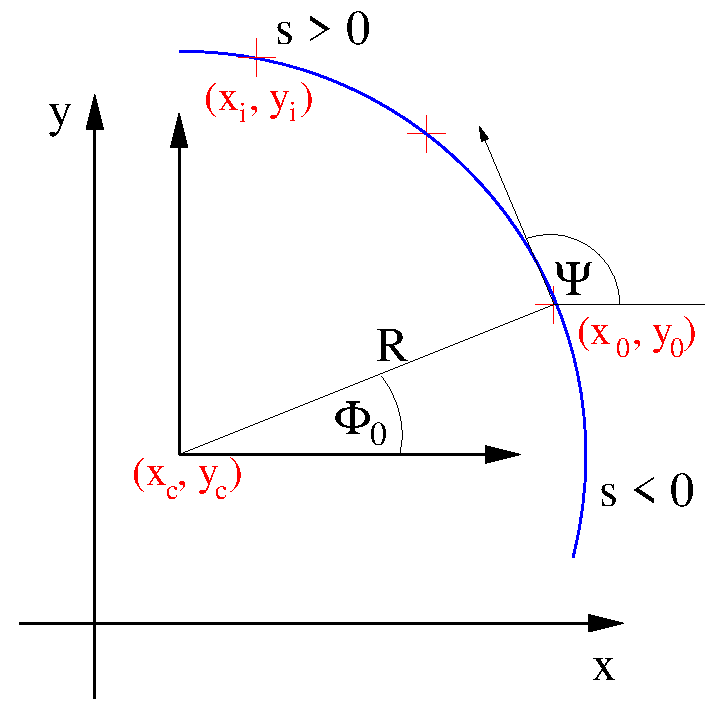
\includegraphics[width=0.45\textwidth]{helix1.eps}}\quad
  \subfigure[Projection of a helix on the $sz$ plane.]{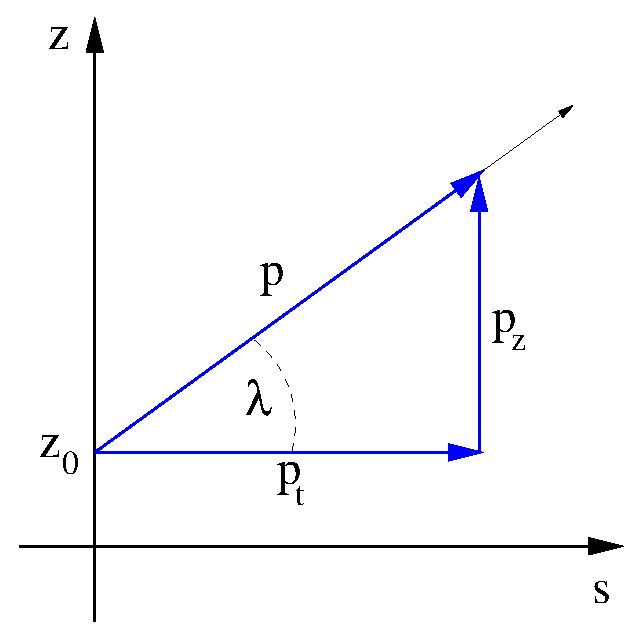
\includegraphics[width=0.45\textwidth]{helix2.eps}}}
  \caption{Helix parametrization}
  \label{fig:helix}
\end{figure}

\subsection{Calculation of the particle momentum}

The circle fit in the $xy$-plane gives the center of the fitted circle $(x_c, y_c)$
and the curvature $\kappa = 1/R$ while the linear fit gives $z_0$ and $\tan \lambda$.
The phase of the helix is defined as follows:
\begin{eqnarray}
  \Phi_0 = \arctan \left( \frac{y_1 - y_c}{x_1 - x_c} \right)
\end{eqnarray}
The reference point $(x_0, y_0)$ is then calculated as follows:
\begin{eqnarray}
  x_0 & = & x_c + \frac{\cos \Phi_0}{\kappa} \\
  y_0 & = & y_c + \frac{\sin \Phi_0}{\kappa}
\end{eqnarray}
and the helix parameters can be evaluated as:
\begin{eqnarray}
  \Psi & = & \Phi_0 + h \pi / 2 \\
  p_\perp & = & c\ q\ B / \kappa \\
  p_z & = & p_\perp \tan \lambda \\
  p & = & \sqrt{p^2_\perp + p^2_z}
\end{eqnarray}
where $\kappa$ is the curvature in [m$^{-1}$], $B$ the value of the
magnetic field in [Tesla], $c$ the speed of light in [m/ns] ($\approx
0.3$) and $p_\perp$ and $p_z$ are the transverse and longitudinal
momentum in [GeV/c].

\subsection{Distant measure}
\index{distance of closest approach}
\index{dca}
The minimal squared distance $M_i$ between a helix and a
point $i$ with position $(x_i, y_i, z_i)$ is given by
\begin{eqnarray}
     M_i & = & M_i^{(xy)} + M_i^{(z)} \\
     M_i & = & (x_i - x(s^\prime))^2 + (y_i - y(s^\prime))^2 + (z_i - z(s^\prime))^2 \\
\end{eqnarray}
In literature one finds the following approach to solve this problem analytically
by neglecting $M_i^{(z)}$ in the derivatives.
\begin{eqnarray}
\frac{\mathrm{d}M_i^{xy}}{\mathrm{d}s}  = 0
\end{eqnarray}
This formula can only serve to derive an approximation for the real distance.
For large dip angles the errors become large depending also on the actual helix
parameters. The advantage is that $s^\prime$ can be calculated analytically:
\begin{eqnarray}
  s^\prime = \frac{1}{h \kappa \cos\lambda} \arctan \left(
    \frac{(y_i-y_0)\cos\Phi_0 - (x_i-x_0) \sin\Phi_0}
    {1/\kappa + (x_i-x_0) \cos\Phi_0 + (y_i-y_0)\sin\Phi_0} \right) \label{eq:dist}
\end{eqnarray}
Note, that this formula can {\bf not} be used to derive the distance of closest
approach to a point.
In order to derive the distance of closest approach the following equation
has to be solved:
\begin{eqnarray}
\frac{\mathrm{d}M_i}{\mathrm{d}s}  = 0
\end{eqnarray}
which can be written as
\begin{eqnarray}
&&2\,\left (x_i-x_0-{\frac {\cos(\Phi_0+h s
  \kappa\cos\lambda)-\cos\Phi_0}{\kappa}}\right) 
  \sin(\Phi_0+h s \kappa\cos\lambda)\ h\cos\lambda -  \nonumber \\
&&2\,\left (y_i-y_0-{\frac {\sin(\Phi_0+h s \kappa\cos\lambda)-\sin
  \Phi_0}{\kappa}}\right) 
  \cos(\Phi_0+ h s \kappa\cos\lambda)\ h\cos\lambda- \nonumber \\
&&2\,\left(z_i-z_0-s\sin\lambda\right )\sin\lambda = 0   \label{eq:dsolve}
\end{eqnarray}
The root of eq.~\ref{eq:dsolve} can easily be found with the Newton or
{\it regula falsi} method
with $s^\prime$ from eq.~\ref{eq:dist} as starting value.
For the Newton method the second derivative is needed as well.
\begin{eqnarray}
\frac{\mathrm{d}^2M_i}{\mathrm{d}s^2}  = 0
\end{eqnarray}
which is
\begin{eqnarray}
    &2&\left (\sin(\Phi_0+hs\kappa\cos\lambda)\right )^{2}{h}^{2}\cos^{2}\lambda + \nonumber \\
    &2&\left (x_i-{x_0}-{\frac {\cos(\Phi_0+hs\kappa\cos\lambda)-\cos\Phi_0}{\kappa}}\right ) \nonumber \\
    & &\cos(\Phi_0+hs\kappa\cos\lambda){h}^{2}\kappa \cos^{2}\lambda + \nonumber \\
    &2&\left (\cos(\Phi_0+hs\kappa\cos\lambda)\right )^{2}{h}^{2}\cos^{2}\lambda +  \nonumber \\
    &2&\left (y_i-{y_0}-{\frac {\sin(
                \Phi_0+hs\kappa\cos\lambda)-\sin\Phi_0}{\kappa}}\right ) \nonumber \\
    & &\sin(\Phi_0+hs\kappa\cos\lambda){h}^{2}\kappa
    \cos^{2}\lambda + \nonumber \\
    &2&\sin^2\lambda = 0 
\end{eqnarray}

\subsection{Distance of closest approach between two helices}
\index{dca between helices} The closest distance between two helices
$H_1$ and $H_2$ is a problem which again can be solved analytically
only in 2 dimensions, i.e., in the xy-plane.  The solution in 3
dimensions cannot even be solved by standard numerical methods (as the
Newton method) but requires more sophisticated method since we have to
find 2 unknown parameters $s_1$ and $s_2$ in
\begin{eqnarray}
\frac{\mathrm{d}^2 M(s_1, s_2)}{\mathrm{d} s_1 \mathrm{d} s_2} = 0
\end{eqnarray}
where $M$ is the distance between the two helices at $s_1$ and $s_2$.

\begin{figure}[hbt]  
    \begin{center}
        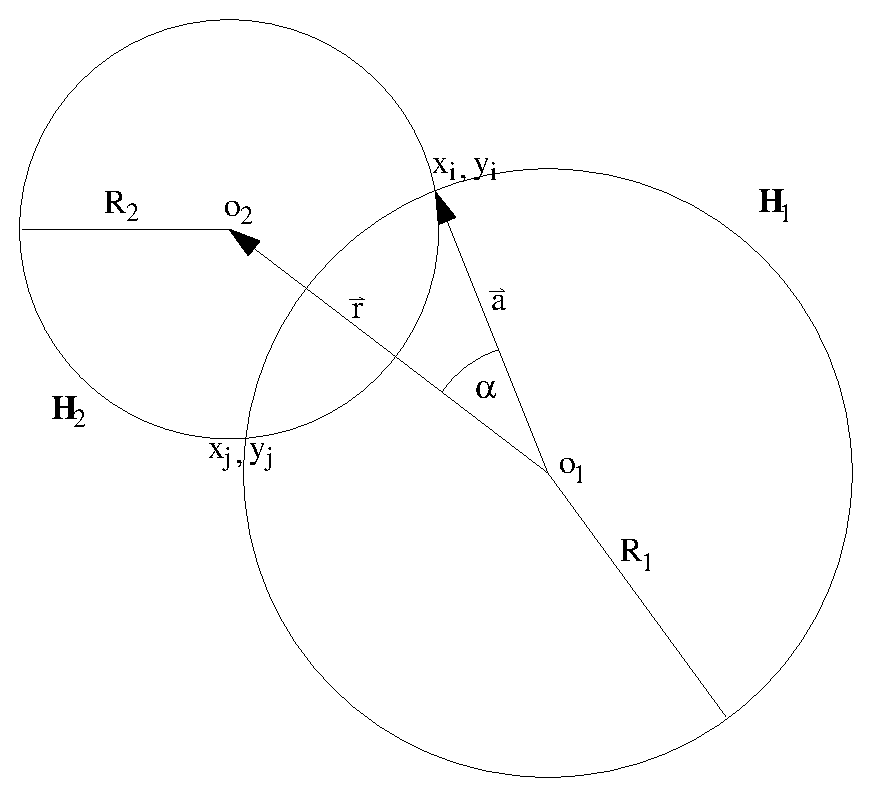
\includegraphics[width=0.5\textwidth]{twoHelices.eps}
        \caption{Two intersecting helices in the xy-plane}
    \end{center}
    \label{fig:dcahelices}
\end{figure}
{\bf In the xy-plane:}\\
Given two helices with radii $R_1$ and $R_2$ and centers in the
xy-plane $o_1 = (x_{c1}, y_{c1})$ and $o_2 = (x_{c2}, y_{c2})$ we have
to find vector $\vec{a}$ as depicted in Fig.\ref{fig:dcahelices}.  The
angle $\alpha$ can be calculated as:
\begin{eqnarray}
    \cos \alpha = \frac{R^2_1 + |\vec{r}|^2 - R^2_2}{2 R_1 |\vec{r}|}
\end{eqnarray}
where $\vec{r}$ is the vector between the two centers. The absolute
coordinates of one intersection point (measured from $o_1$) can be
obtained by calculating vector $\vec{a}$ and adding $o_1$.
\begin{eqnarray}
    x_i &=& x_{c1} + R_1 [ (x_{c2}-x_{c1}) \cos \alpha -  (y_{c2}-y_{c1}) \sin \alpha]/|\vec{r}|;\\
    y_i &=& y_{c1} + R_1 [ (x_{c2}-x_{c1}) \sin \alpha +  (y_{c2}-y_{c1}) \cos \alpha]/|\vec{r}|;
\end{eqnarray}
If $\cos \alpha$ is exactly 1 we have only one solution. For the case
$\cos \alpha < 1$ we get two valid intersection points $(x_i, y_i)$
and $(x_j, y_j)$ where the latter is simply given by:
\begin{eqnarray}
    x_j &=& x_{c1} + R_1 [ (x_{c2}-x_{c1}) \cos \alpha +  (y_{c2}-y_{c1}) \sin \alpha]/|\vec{r}|;\\
    y_j &=& y_{c1} + R_1 [ (y_{c2}-y_{c1}) \cos \alpha -  (x_{c2}-x_{c1}) \sin \alpha]/|\vec{r}|;
\end{eqnarray}
In the case $\cos \alpha > 1$ the circles do not intersect. Then the
distance of closest approach is simply given by the intersection of a
line between the two centers and the two helices. For helix $H_1$ we
get:
\begin{eqnarray}
    x &=& x_{c1} + R_1 (x_{c2}-x_{c1})/|\vec{r}|;\\
    y &=& y_{c1} + R_1 (y_{c2}-y_{c1})/|\vec{r}|;
\end{eqnarray}


{\bf In 3 dimensions:}\\
Usually an iteration method is applied which uses the intersection
points in the xy-plane as start values. Care has to be taken if both
helices have different dip angle $\lambda$ since the start values then
significantly deviate from the actual solution.

\subsection{Intersection with a cylinder ($\rho$=const)}

In order to obtain the path length $s$ at which the helix
intersects with a cylinder of given radius $\rho$ we have to solve
the following equation:
\begin{eqnarray}
    \rho^2 = x(s)^2 + y(s)^2
\end{eqnarray}
Using eq.~\ref{eq:xs} and \ref{eq:ys} we obtain the two analytic solutions for $s_1$ and $s_2$:
\begin{eqnarray} \label{eq:rsolve}
    s_{1/2} &=& -\left({\Phi_0}+2\,\arctan \left[
            \left(2\,{y_0}\,\kappa-2\,\sin{\Phi_0} \pm \left[ -
                    \kappa^2\left (-4\,\rho^2+4\,{y_0}^2 - 2\,\rho^2\kappa^2 x_0^2 -  
                    \right. \right. \right. \right. \right. \\ \nonumber
    & & \left. \left. \left. \left. \left.
                        2\,\rho^2 \kappa^2 {y_0}^{2} + 2\,{{x_0}}^{2}{\kappa}^{2}{
                            {y_0}}^{2}+{\rho}^{4}{\kappa}^{2}+{{x_0}}^{4}{\kappa}^{2}+{{y_0}}^{4}{
                            \kappa}^{2}-4\,{{x_0}}^{3}\kappa\,\cos{\Phi_0} +
                    \right. \right. \right. \right. \right. \\ \nonumber
    & & \left. \left. \left. \left. \left.
                        4\,{{x_0}}^{2}\cos^2{\Phi_0} - 4\,{{y_0}}^{2} \cos^{2}{\Phi_0} -
                    \right. \right. \right. \right. \right. \\ \nonumber
    & & \left. \left. \left. \left. \left.
                        4\,{{y_0}}
                        ^{3}\kappa\,\sin{\Phi_0}+4\,{\rho}^{2}\kappa\,{x_0}\,\cos{\Phi_0}\, + 4\,{\rho}^{2}\kappa
                        \,{y_0}\,\sin{\Phi_0}\, -4\,{{x_0}}^{2}\kappa\,{y_0}\,\sin{\Phi_0} -
                    \right. \right. \right. \right. \right. \\ \nonumber
    & & \left. \left. \left. \left. \left.
                        4\,{{y_0}}^{2}\kappa\,{x_0}\,\cos{\Phi_0}\, +8\,{x_0}\,\cos{\Phi_0}\,{y_0}\,\sin{\Phi_0}
                    \right ) \right]^{1/2} \right) /
        \right. \right. \\ \nonumber
    & & \left. \left.
            \left(
                -{\rho}^{2}{\kappa}^{2}+2+{x_0}^{2}{\kappa}^{2}+2\,\cos{\Phi_0}+{y_0}^{2}{\kappa}^{2} -
            \right. \right. \right. \\ \nonumber
    & & \left. \left. \left.
                2\,{x_0}\,\kappa-2\,{x_0}\,\kappa\,\cos{\Phi_0}\,
                -2\,{y_0}\,\kappa\,\sin{\Phi_0} \right)
        \right] \right){h}^{-1}{\kappa}^{-1}\left (
        \cos\lambda\right )^{-1}
\end{eqnarray}


\subsection{Intersection with a plane}

\begin{figure}[thb]
    \begin{center}
        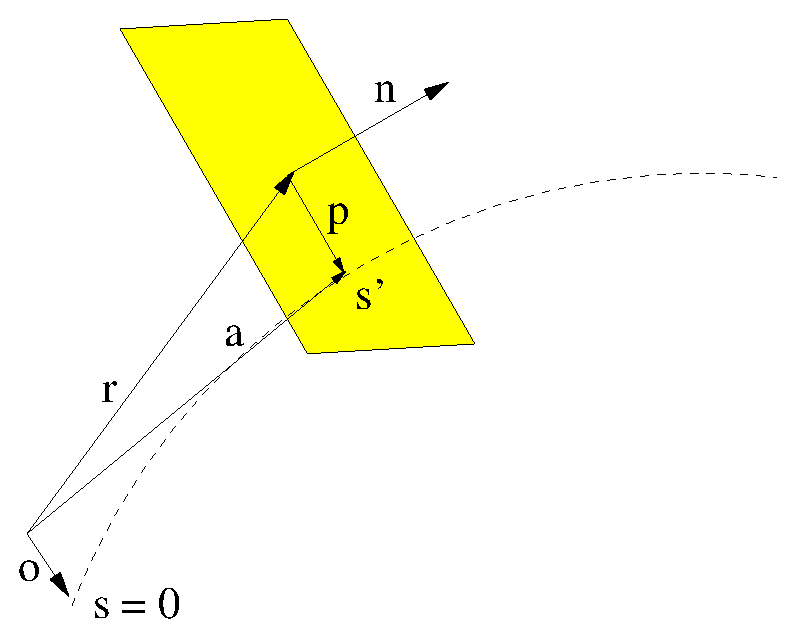
\includegraphics[width=0.6\textwidth]{helix3.eps}
        \caption{Intersection of a helix with a plane}
        \label{fig:plane}
    \end{center}
\end{figure}

Any plane can be described by its normal vector $\vec{n}$
(orientation) and an arbitrary point in this plane $\vec{r}$ (position). The vector
$\vec{p}$ which describes the intersection point must fulfil:
\begin{eqnarray}
    \vec{p} \cdot \vec{n} = 0.
\end{eqnarray}
Hence:
\begin{eqnarray}
    (\vec{a}-\vec{r}) \cdot \vec{n} = 0. \label{eq:ansatz}
\end{eqnarray}
where $\vec{a}$ is given by $\vec{a} = (x(s^{\prime}),
y(s^{\prime}), z(s^{\prime}))$ as described in
eq.~\ref{eq:xs}--\ref{eq:zs}.  In order to obtain the path length
$s^{\prime}$ where the helix intersects with the plane the
following equation has to be solved:
\begin{eqnarray}
    x(s) n_x + y(s) n_y + z(s) n_z - \vec{r} \cdot \vec{n} &=& \\
    A + n_x \cos S
    + n_y \sin S
    + \kappa n_z s \sin \lambda &=& 0 \label{eq:inter}
\end{eqnarray}

\begin{eqnarray}
    A &=& \kappa (\vec{o} \cdot \vec{n} - \vec{r} \cdot \vec{n}) - n_x \cos \Phi_0 - n_y \sin \Phi_0 \\
    S &=& h s \kappa \cos \lambda + \Phi_0  
\end{eqnarray}

The root of eq.~\ref{eq:inter} can now easily be determined by a
suitable numerical method (Newton).

\subsection{Limitations}
\label{sec:Limitations}
The only non-numerical limitations of this parametrization are:
\begin{eqnarray}
    -\pi/2 < \lambda  & < & \pi/2 \\
    x(s) & = & x_0 - s \cos\lambda \sin\Phi_0 \\
\textbf{Important:} For $B = 0$ the sense of rotation is ill defined. Here
we arbitrarily set $h = +1$. This implies that $\Phi_0 = \Psi - \pi/2$.
calculation of the parametrization because of the singularity in
eq.~\ref{eq:xs} and \ref{eq:ys}. The correct form is:
\begin{eqnarray}
    x(s) & = & x_0 - s h \cos\lambda \sin\Phi_0 \\
    y(s) & = & y_0 + s h \cos\lambda \cos\Phi_0 \\
    z(s) & = & z_0 + s\ \sin\lambda
\end{eqnarray}
\textbf{Important:} For $B = 0$ the sense of rotation is ill defined. All what matters
is that $\Phi_0 = \Psi - h \pi/2$ is done correctly, i.e.~with the same arbitrary $h$. 
In the following we assume $h = +1$ for convenience.

Eq.~\ref{eq:dist} then reads as:
\begin{eqnarray}
  s^\prime = \frac{1}{\cos\lambda} \left[(y_i-y_0)\cos\Phi_0 - (x_i-x_0) \sin\Phi_0 \right]
\end{eqnarray}
Eq.~\ref{eq:dsolve} can now be solved analytically;
\begin{eqnarray}
\frac{\mathrm{d}M_i^{dca}}{\mathrm{d}s} = 0
\end{eqnarray}
gives:
\begin{eqnarray}
s^{dca}   & = & \cos\lambda \cos\Phi_0 (y_i-y_0) - \nonumber \\
          &   & \cos\lambda \sin\Phi_0 (x_i-x_0) + \nonumber \\
          &   & \sin\lambda (z_i-z_0)
\end{eqnarray}

The solution for the intersection with a cylinder (eq.~\ref{eq:rsolve}) now reads:
\begin{eqnarray}
s_{1/2}   & = & \left[x_0\,\cos\lambda\,\sin\Phi_0\,- y_0\,\cos\lambda\,\cos\Phi_0 \, \pm  \right. \\
   & & \left.
\left[-\cos^2\lambda\,\left(2\,x_0\,\cos\Phi_0\, y_0
\,\sin\Phi_0\,-\rho^2\, + \right. \right. \right.  \\
& & \left. \left.  \left.
y_0^2-y_0^2 \,\cos^2\Phi_0\,
+ x_0^2  \cos^2\Phi_0 \right )\right]^{1/2} \right]\, \cos^2\lambda 
\end{eqnarray}


The same holds for the intersection of a helix with a plane where in case
of zero curvature eq.~\ref{eq:inter} can be solved analytically.
\begin{eqnarray}
s^{\prime} = \frac{ \vec{r} \cdot \vec{n} - \vec{o} \cdot \vec{n} }
                  {- n_x \cos \lambda \sin \Phi_0
                   + n_y \cos \lambda \cos \Phi_0
                   + n_z \sin \lambda}
\end{eqnarray}

\subsection{Why are there only 5 independent helix parameters?}
\label{sec:hparam}
    
    Imagine an arbitrary helix sitting in 3D space.  What is required
    to completely specify it ?
    \begin{enumerate}
    \item the line coinciding with the axis - if its oriented in any arbitrary
        direction, then this requires 4 parameters, or 2 direction angles
        (theta and phi in usual spherical coordinates) plus 2 more coordinates
        to locate the line in a plane perpendicular to this direction.
       
        For the special case in STAR we always fix the direction 
        parallel to the z-axis so this reduces the number of this subset
        of parameters from 4 to 2.

        So these are the (x,y) coordinates of the center of the circular
        projection onto the x-y plane.

    \item Then we must give the radius of the circular projection - 1 more param,
                 
    \item Next we must specify the pitch and the handedness. - 2 more params.

    \item  Finally, we have to give a phase angle or some single number that
        tells us where this thing is actually sitting w.r.t. some given
        plane.  For STAR this could be the phase angle at the point where
        the helix intersects the x-y plane. - 1 more parameter.
        
    \end{enumerate}

    So, in general there are 7 continuously varying parameters plus a 
    handedness switch.  For the special case STAR uses there are then
    5 independent parameters plus the left handed/right handed
    switch. So yes, 6 parameters are required.  But for track fitting
    purposes only 5 are relevant.  The handedness of the particle's
    trajectory will be determined by the
    sign of B$_z \times $ charge (using the actual charge) and the sign of the
    z-component of momentum (using the actual p$_z$ momentum value).
    However, in general the charge sign and p$_z$ direction are not
    known, based on track fitting alone.  These signs must be assumed
    using some selection criteria, usually that the particle is moving
    ``outward and away'' from the general area of the beam.  These two signs
    are not independent of each other but must be chosen to give a path
    consistent with the handedness that the space point positions require.
    So there is one algebraic sign that is ambiguous and that we have to
    choose.  Having done this there remain 5 independent fitting parameters.
    In our track parametrization we put the choice of algebraic sign
    into the both that of the charge and the tanl parameter, consistently
    we hope.

    So to summarize, there are 6 parameters, one is a sign selected by some
    criteria, the remaining 5 are varied to fit the space points.
    The track parameter error matrix is then $5 \times 5$ symmetric, and thus
    includes 15 distinct quantities.

    \hfill\textit{Text from Lanny Ray written during an email exchange on this very topic.}

%%%%%%%%%%%%%%%%%%%%%%%%%%%%%%%%%%%%%%%%%%%%%%%%%%%%%%%%%%%%%%%%%%%%
%
% The End
%
%%%%%%%%%%%%%%%%%%%%%%%%%%%%%%%%%%%%%%%%%%%%%%%%%%%%%%%%%%%%%%%%%%%%

\printindex

\end{document}
